

\appendix
%\renewcommand{\thechapter}{A}
 \refstepcounter{chapter}
    \makeatletter
   \renewcommand{\theequation}{\thechapter.\@arabic\c@equation}
    \makeatother
\chapter*{Appendices}
\label{app}
\addcontentsline{toc}{chapter}{Appendices}
%\begin{comment}

\renewcommand{\thesection}{A}
 \refstepcounter{section}
    \makeatletter
   \renewcommand{\theequation}{\thesection.\@arabic\c@equation}
    \makeatother
\section*{Appendix A: Features of missing mass distributions}
\label{app_mm_features}
\addcontentsline{toc}{section}{A: Features of missing mass distributions}

Let's consider the double-pion electroproduction off the free proton $ep\rightarrow e'p'\pi^{+}\pi^{-}$ and define the following missing quantities,\vspace{-0.5em}
\begin{equation}
\begin{aligned}
&M_{X[0]}^{2}&=&\left [P_{X[0]}^{\mu} \right ]^{2}&=&~\left [P_{e}^{\mu} + P_{p}^{\mu}- P_{e'}^{\mu}- P_{p'}^{\mu}-  P_{\pi^{+}}^{\mu} - P_{\pi^{-}}^{\mu}\right ]^{2},\\
&M_{X[\pi^{-}]}^{2}&=&\left [P_{X[\pi^{-}]}^{\mu}\right ]^{2}&=&~\left [P_{e}^{\mu} + P_{p}^{\mu}- P_{e'}^{\mu}- P_{p'}^{\mu}-  P_{\pi^{+}}^{\mu}\right ]^{2},\\[-7pt]
\end{aligned}\label{eq:mm_def}
\end{equation}
where $P_{X[0]}^{\mu}$ and $P_{X[\pi^{-}]}^{\mu}$ are the corresponding missing four-vectors, while $P_{i}^{\mu}$ is the four-momentum of the particle $i$.
\begin{figure}[htp]
\begin{center}
\framebox{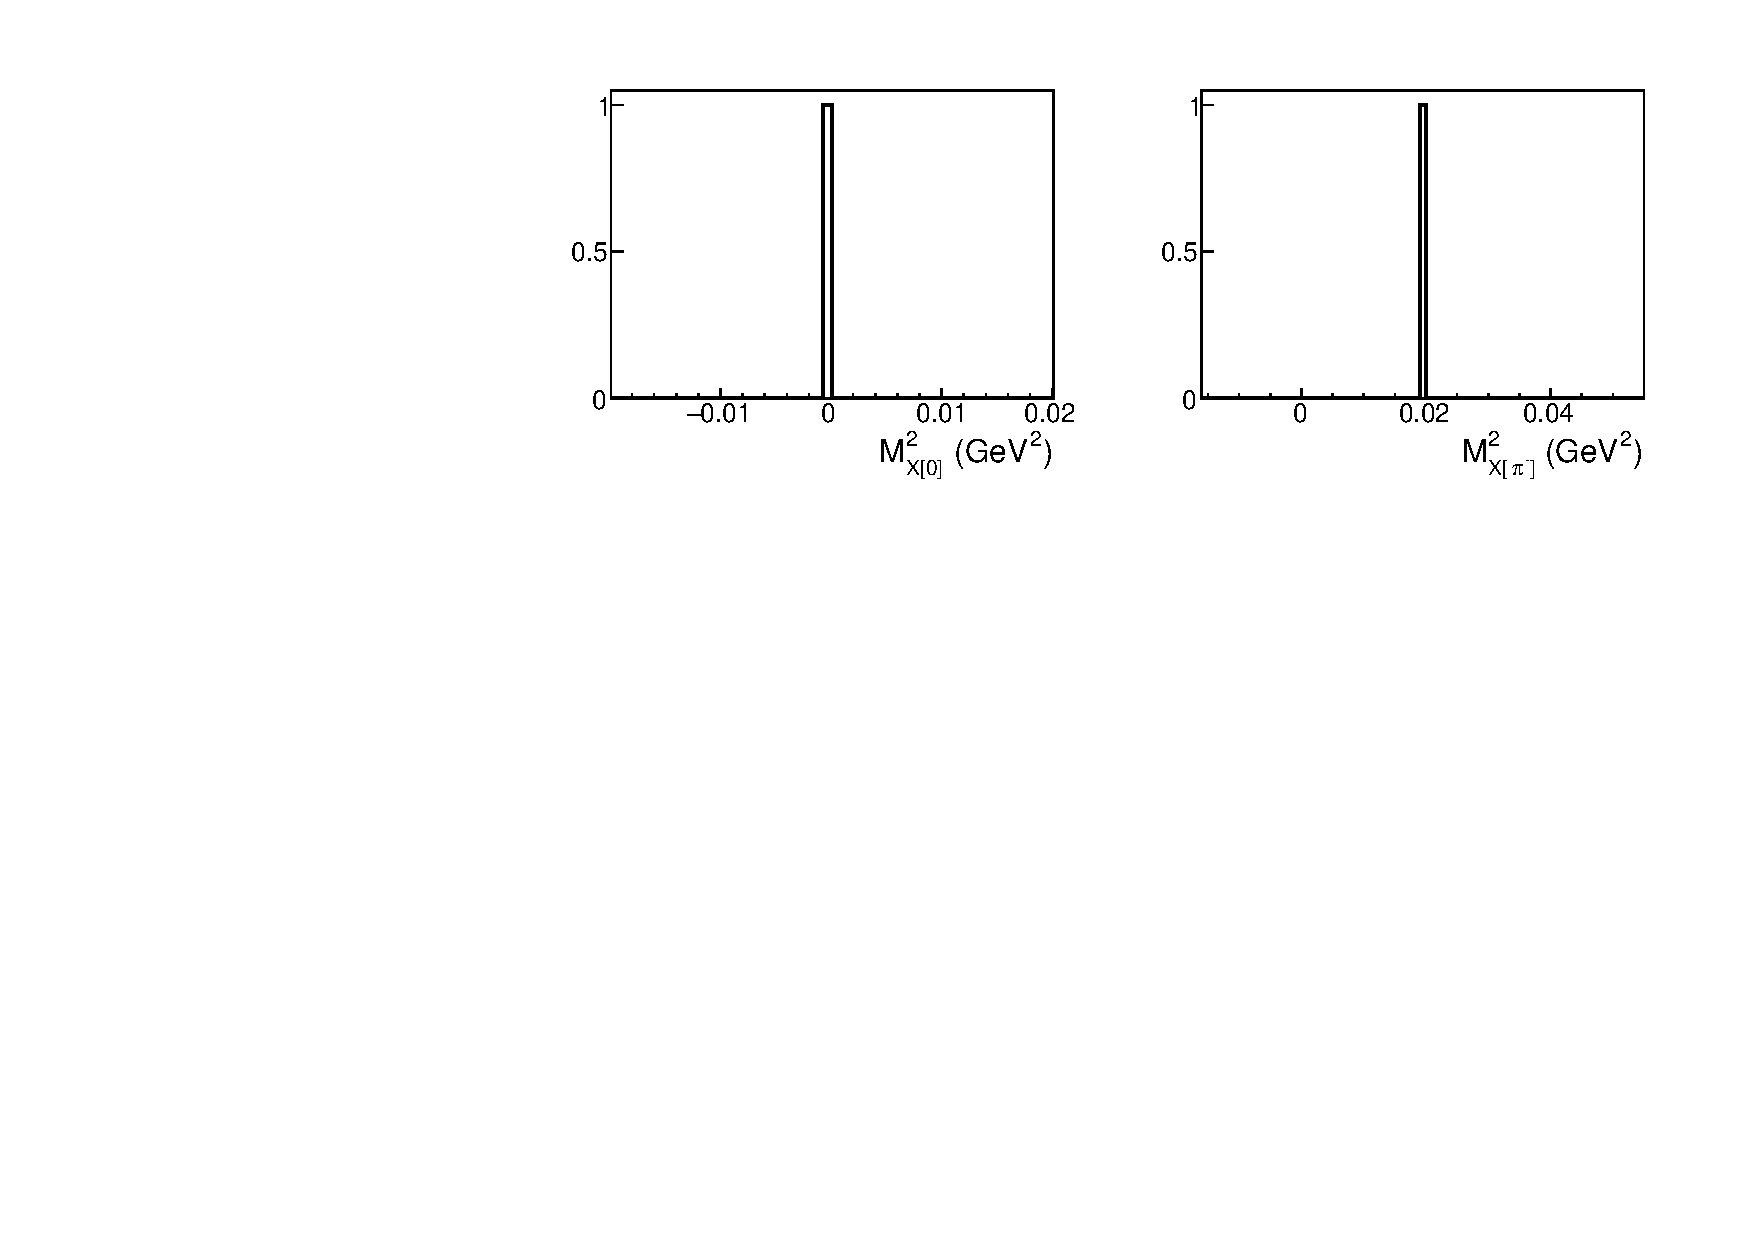
\includegraphics[width=0.795\textwidth]{pictures/appendix/mm_norad_nofsi.pdf}}
\caption{\small Quantities $M_{X[0]}^{2}$ (left) and $M_{X[\pi^{-}]}^{2}$ (right).} \label{fig:norad_nofsi}
\end{center}
\end{figure}

\vspace{-1.5em}
Let's firstly assume that (i) all events in the sample correspond to the reaction $ep\rightarrow e'p'\pi^{+}\pi^{-}$, (ii) all four-momenta are defined exactly without any resolution uncertainty, and (iii) neither radiative effects nor FSI occur. Then\footnote[1]{Note that for the quantity $M_{X[0]}^{2}$ the missing four-vector in the square brackets in Eqs.~\eqref{eq:mm_def} is equal to zero componentwise, which means that the energy and each momentum component are equal to zero.} \vspace{-0.5em}
\begin{equation}
\begin{aligned}
&M_{X[0]}^{2}&=&~0~~~~\textrm{and}~~~~M_{X[\pi^{-}]}^{2}&=&~[P_{\pi^{-}}^{\mu}]^{2}=m_{\pi}^{2},\\[-7pt]
\end{aligned}\label{eq:rrr}
\end{equation}
which means that both $M_{X[0]}^{2}$ and $M_{X[\pi^{-}]}^{2}$ form a discrete narrow peak at the position of zero and $m_{\pi}^{2}$, respectively, as Fig.~\ref{fig:norad_nofsi} demonstrates\footnote[2]{All histograms in this Appendix are filled with events generated with TWOPEG~\cite{twopeg} for $E_{beam}$ = 2.039~GeV, 1.4~GeV $< W <$ 1.8~GeV and 0.4~GeV$^{2}$ $< Q^{2} <$ 0.6~GeV$^{2}$ (unless specified otherwise). All distributions are normalized in a way that the maxima of the main peaks are equal to one.}.


Now let's trace the impact of different effects on the missing mass distributions.
\vspace{-0.75em}
\subsection* {Radiative effects}
\vspace{-0.5em}
Let's calculate the quantities $M_{X[0]}^{2}$ and $M_{X[\pi^{-}]}^{2}$ assuming that either the incoming or scattered electron can emit a radiative photon, and (if the emission occurs) $P_{e}^{\mu}$/$P_{e'}^{\mu}$ in Eqs.~\eqref{eq:mm_def} is the four-momentum of the incoming/scattered electron determined before/after the emission, respectively. Then for events with the photon emission\vspace{-0.5em}
\begin{equation}
\begin{aligned}
&M_{X[0]}^{2}&=&~[P^{\mu}_{\gamma}]^{2} = 0~~\textrm{and}\\[8pt]
&M_{X[\pi^{-}]}^{2}&=&~[P_{\pi^{-}}^{\mu}+P^{\mu}_{\gamma}]^{2}=[P^{\mu}_{\pi^{-}}]^{2} +[P^{\mu}_{\gamma}]^{2}+2(P^{\mu}_{\pi^{-}}\cdot P^{\mu}_{\gamma} ) =\\
&&=&~m_{\pi}^{2} +2(E_{\pi^{-}}E_{\gamma} - (\overrightarrow{p}_{\pi^{-}}\cdot \overrightarrow{p}_{\gamma})) = \\
&&=&~m_{\pi}^{2} +2(E_{\pi^{-}}E_{\gamma} - |\overrightarrow{p}_{\pi^{-}}|E_{\gamma}cos\beta) =\\
&&=&~ m_{\pi}^{2} +2E_{\gamma}(E_{\pi^{-}} -|\overrightarrow{p}_{\pi^{-}}|cos\beta ) >m_{\pi}^{2}   ,\\[-7pt]
\end{aligned}\label{eq:mm_rad}
\end{equation}
where $\beta$ corresponds to the angle between the $\pi^{-}$ and the emitted radiative photon.

\begin{figure}[htp]
\begin{center}
\framebox{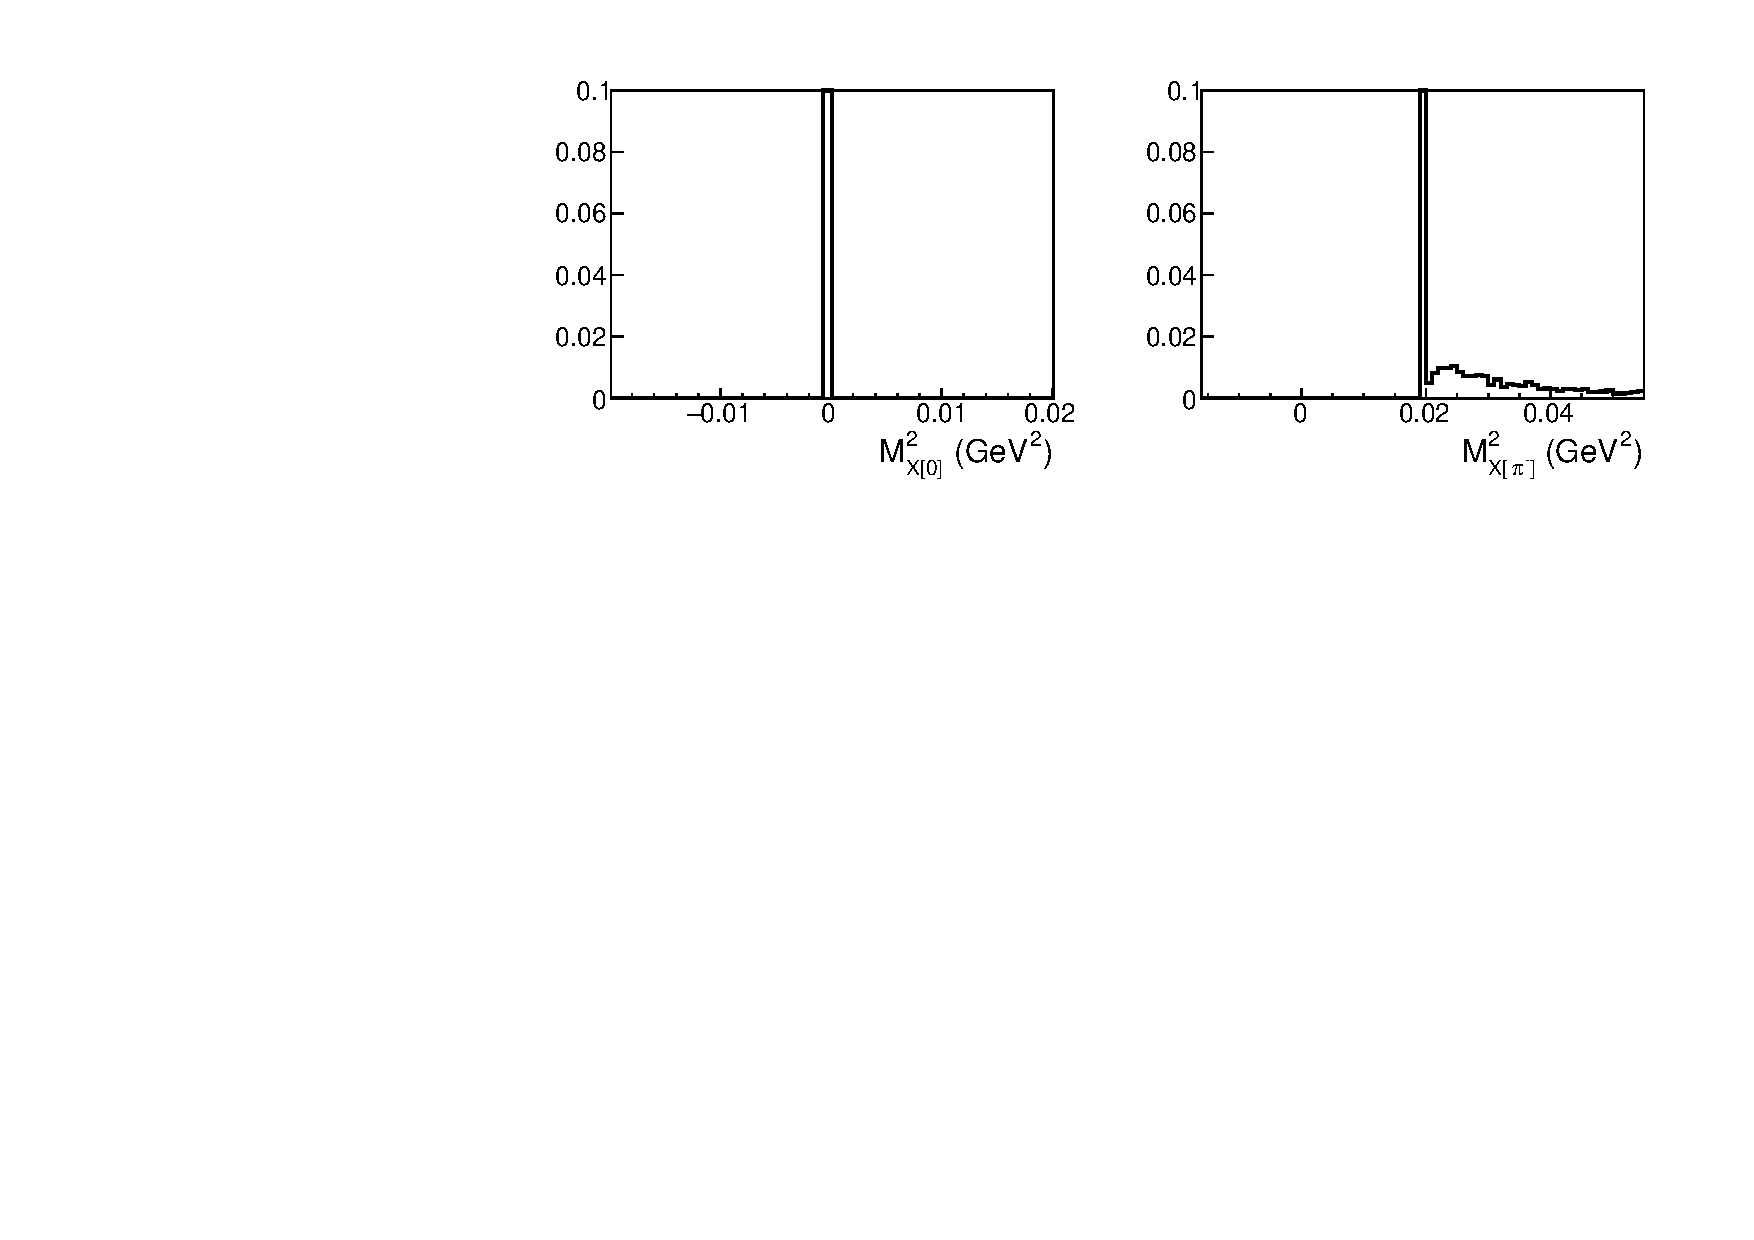
\includegraphics[width=0.795\textwidth]{pictures/appendix/mm_rad_nofsi.pdf}}
\caption{\small Impact of radiative effects on $M_{X[0]}^{2}$ (left) and $M_{X[\pi^{-}]}^{2}$ (right). Both distributions are zoomed in onto small $y$ to make the impact of the radiative effects visible.} \label{fig:mm_rad}
\end{center}
\end{figure}

\vspace{-1.5em}
As follows from Eqs.~\eqref{eq:mm_rad}, the quantity $M_{X[0]}^{2}$ feels no impact of the radiative photon emission\footnote[3]{Note that for the quantity $M_{X[0]}^{2}$ the missing four-vector in the square brackets in Eqs.~\eqref{eq:mm_def} is the four-momentum of the radiative photon, which is not equal to zero componentwise. However, being massless, the photon has the energy equal to its momentum magnitude, which gives zero upon the calculation of $M_{X[0]}^{2}$. Thus the zero value of $M_{X[0]}^{2}$ has a different nature for events with and without radiative effects.}, while the quantity $M_{X[\pi^{-}]}^{2}$ acquires a right-side tail, which is demonstrated in Fig.~\ref{fig:mm_rad}.


\vspace{-0.75em}
\subsection*{Admixture from other channels}
\vspace{-0.5em}
Let's assume that some events in the sample correspond to the background channel with greater amount of final state particles, i.e. $ep\rightarrow e'p'\pi^{+}\pi^{-}x$. Then for the background events\vspace{-0.5em}
\begin{equation}
\begin{aligned}
&M_{X[0]}^{2}&=&~[P^{\mu}_{x}]^{2} = m_{x}^{2} >0~~\textrm{and}\\[8pt]
&M_{X[\pi^{-}]}^{2}&=&~[P_{\pi^{-}}^{\mu}+P^{\mu}_{x}]^{2}=[P^{\mu}_{\pi^{-}}]^{2} +[P^{\mu}_{x}]^{2}+2(P^{\mu}_{\pi^{-}}\cdot P^{\mu}_{x} ) =\\
&&=&~m_{\pi}^{2} + m_{x}^{2} +2(E_{\pi^{-}}E_{x} - (\overrightarrow{p}_{\pi^{-}}\cdot \overrightarrow{p}_{x})) > \\
&&>&~m_{\pi}^{2} + m_{x}^{2}+2m_{\pi}m_{x} > m_{\pi}^{2},\\[-7pt]
\end{aligned}\label{eq:mm_other_ch}
\end{equation}
which means that background events form an additional right-side peak well-separated from the main one by $m_{x}^{2}$ and $m_{x}^{2}+2m_{\pi}m_{x}$ for $M_{X[0]}^{2}$ and $M_{X[\pi^{-}]}^{2}$, respectively.

This situation is illustrated in Fig.~\ref{fig:mm_backgr} for the case when the background channel is $ep\rightarrow e'p'\pi^{+}\pi^{-}\pi^{0}$.

\begin{figure}[htp]
\begin{center}
\framebox{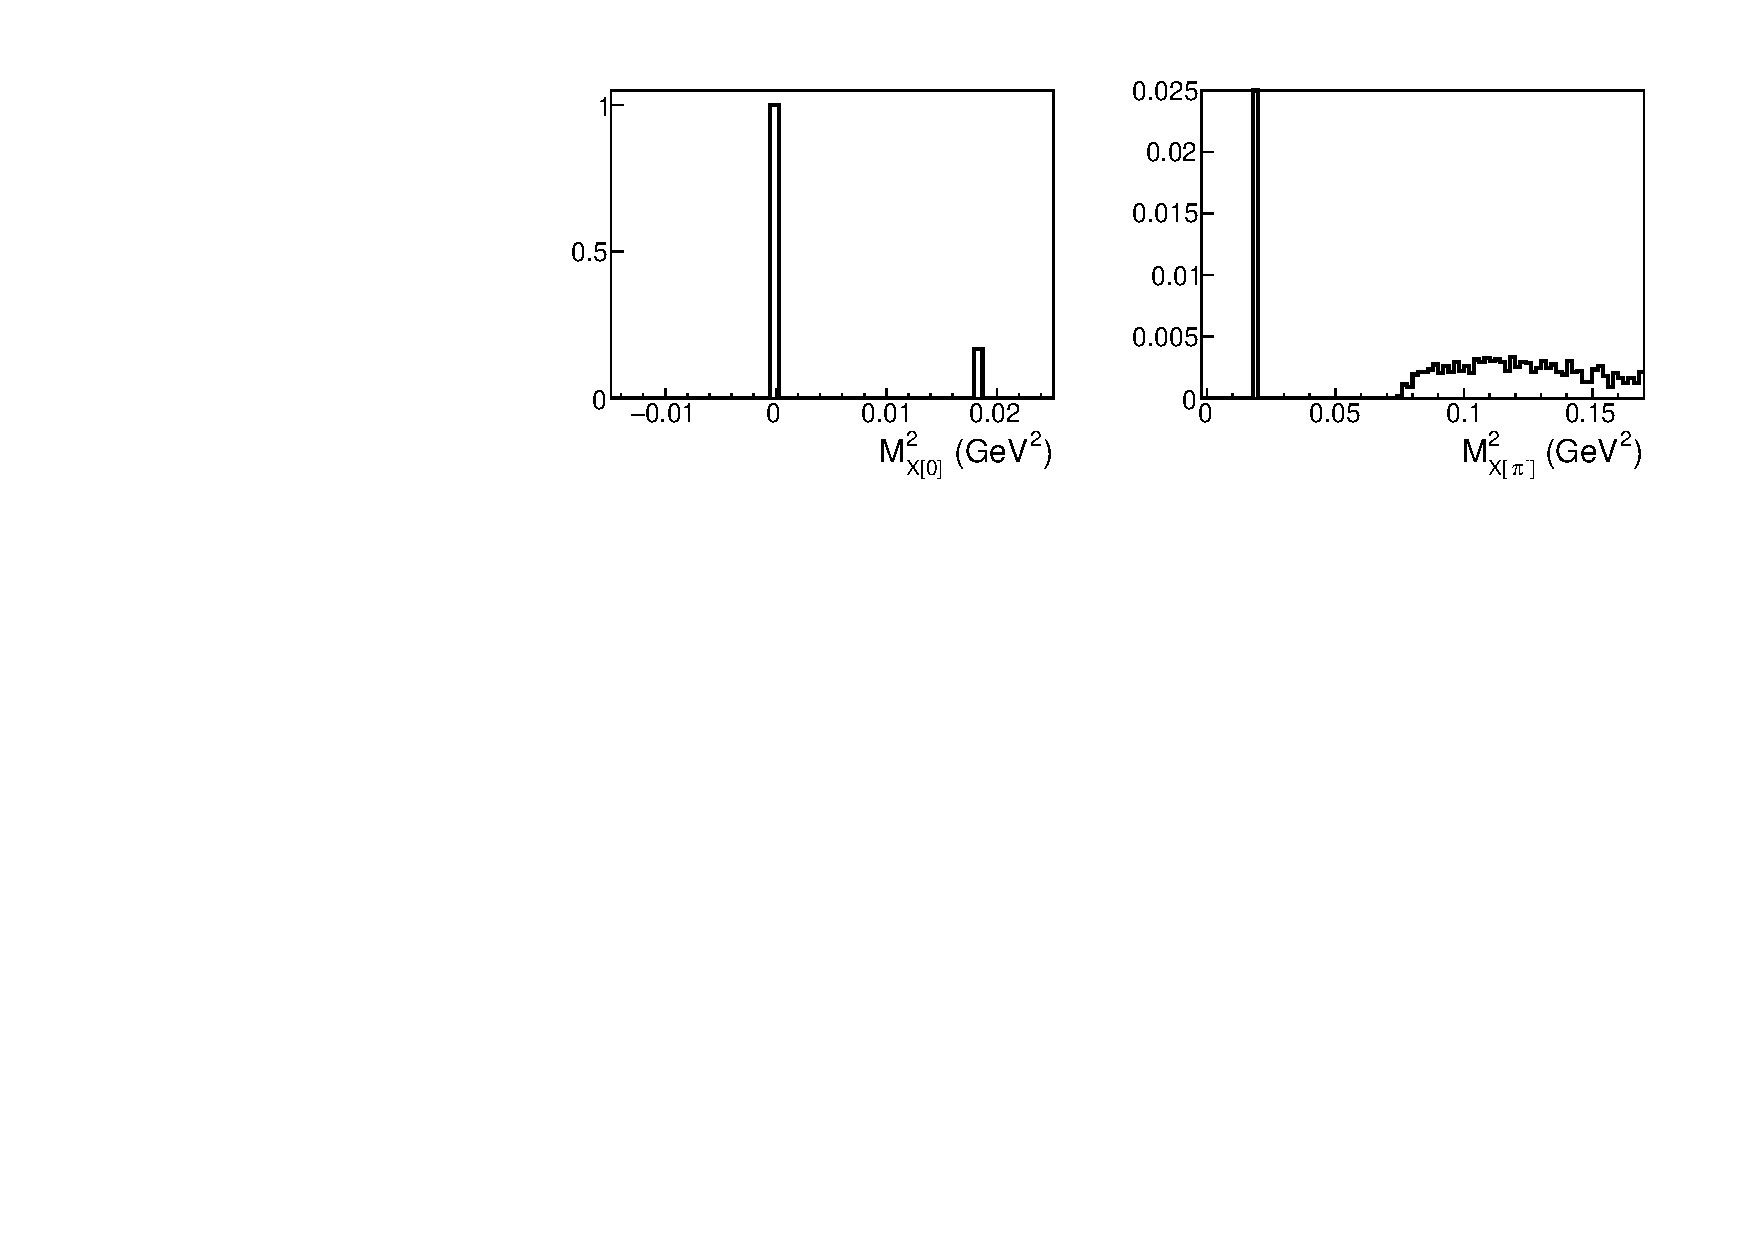
\includegraphics[width=0.8\textwidth]{pictures/appendix/mm_other_ch.pdf}}
\caption{\small Quantities $M_{X[0]}^{2}$ (left) and $M_{X[\pi^{-}]}^{2}$ (right) plotted for the case when the event sample has an admixture from the background channel $ep\rightarrow e'p'\pi^{+}\pi^{-}\pi^{0}$. The discrete right peak (in the left plot) and the right-side structure (in the right plot), both well-separated from the main peak, correspond to the background events. The right plot is zoomed in onto small $y$. The plots are produced by means of the GENEV event generator~\cite{Genev} for $E_{beam}$ = 2.039~GeV, 1.4~GeV $< W <$ 1.8~GeV and 0.4~GeV$^{2}$ $< Q^{2} <$ 0.6~GeV$^{2}$.  } \label{fig:mm_backgr}
\end{center}
\end{figure}
\vspace{-1.5em}


\vspace{-0.75em}
\subsection* {Detector resolution}
\vspace{-0.5em}
Let's now assume that for all events in the sample the particle four-momenta $P_{i}^{\mu}$ in Eqs.~\eqref{eq:mm_def} are determined with the uncertainty of the detector resolution and then estimate the resulting uncertainties of the missing mass distributions. 

The missing quantity $M_{X}^{2}$ can be written in the following way,\vspace{-0.5em}
\begin{equation}
\begin{aligned}
&M_{X}^{2}&=&~(E_{X})^{2} - (p_{X}^{x})^{2} - (p_{X}^{y})^{2}  -  (p_{X}^{z})^{2} =\\
&&=&~\left (\sum_{\substack{i}} \pm \sqrt{m_{i}^{2}+p_{i}^{2}} \right )^{2} - \left (\sum_{\substack{i}}\pm p_{i}^{x} \right )^{2} - \left (\sum_{\substack{i}}\pm p_{i}^{y} \right )^{2} - \left (\sum_{\substack{i}}\pm p_{i}^{z} \right )^{2},\\[-7pt]
\end{aligned}\label{eq:mm_def2}
\end{equation}
where $E_{X}$ and $p_{X}^{j}$ ($j = x,~y,~z$) are the energy and momentum components of the missing four-vector, while $m_{i}$, $E_{i}$, and $p_{i}^{j}$ are the mass, energy, and momentum components of the individual particles with the index $i$ running over all particles involved in the missing mass calculation (see Eqs.~\eqref{eq:mm_def}). For the $\pm$ sign the plus is taken for the initial particles ($e$ and $p$) and the minus for the final particles.




Then let's estimate the uncertainties of the quantities $E_{X}$ and $p_{X}^{j}$ through the corresponding uncertainties for the individual particles. 
The absolute uncertainties for the energy components $E_{X}$ are given by\vspace{-0.5em}
\begin{equation}
\begin{aligned}
&\Delta E_{X[0]} &=&~\sqrt{ \left ( \Delta E_{e'} \right )^{2} + \left ( \Delta E_{p'} \right )^{2} +  \left ( \Delta E_{\pi^{+}} \right )^{2} + \left ( \Delta E_{\pi^{-}} \right )^{2}} =\\
&&=&~\sqrt{\left ( \Delta p_{e'} \right )^{2} + \left (p_{p'}/E_{p'}\right )^{2} \left (\Delta p_{p'} \right )^{2} +  \left (p_{\pi^{+}}/E_{\pi^{+}}\right )^{2} \left (\Delta p_{\pi^{+}} \right )^{2}+\left (p_{\pi^{-}}/E_{\pi^{-}}\right )^{2} \left (\Delta p_{\pi^{-}} \right )^{2}}, \\[10pt]
&\Delta E_{X[\pi^{-}]} &=&~\sqrt{ \left ( \Delta E_{e'} \right )^{2} + \left ( \Delta E_{p'} \right )^{2} + \left ( \Delta E_{\pi^{+}} \right )^{2}}=\\
&&=&~\sqrt{\left ( \Delta p_{e'} \right )^{2} + \left (p_{p'}/E_{p'}\right )^{2} \left (\Delta p_{p'} \right )^{2} +  \left (p_{\pi^{+}}/E_{\pi^{+}}\right )^{2} \left (\Delta p_{\pi^{+}} \right )^{2}},\\[-7pt]
\end{aligned}\label{eq:res}
\end{equation}
where $\Delta p_{i}$ is the uncertainty of the momentum magnitude for the particle $i$, which comes from the momentum resolution of Drift Chambers (where the momentum magnitude is supposed to be measured).

The absolute uncertainties for the momentum components $p_{X}^{j}$ are in turn\vspace{-0.5em}
\begin{equation}
\begin{aligned}
&\Delta p_{X[0]}^{j} &=&~\sqrt{ \left ( \Delta p_{e'}^{j} \right )^{2} + \left ( \Delta p_{p'}^{j} \right )^{2} +  \left ( \Delta p_{\pi^{+}}^{j} \right )^{2} + \left ( \Delta p_{\pi^{-}}^{j} \right )^{2}}, \\
&\Delta p_{X[\pi^{-}]}^{j} &=&~\sqrt{ \left ( \Delta p_{e'}^{j} \right )^{2} + \left ( \Delta p_{p'}^{j} \right )^{2} +  \left ( \Delta p_{\pi^{+}}^{j} \right )^{2}},\\[-7pt]
\end{aligned}\label{eq:res2}
\end{equation}
where $\Delta p_{i}^{j}$ are the uncertainties of the $j$-components of the particle's three-momenta ($j = x,~y,~z$), which come from both the momentum magnitude resolution and the spatial angular resolution of Drift Chambers.


As follows from Eqs.~\eqref{eq:res} and~\eqref{eq:res2}, $p_{X[0]}^{j}$ and $E_{X[0]}$ acquire larger absolute uncertainties than $p_{X[\pi^{-}]}^{j}$ and $E_{X[\pi^{-}]}$, respectively, as they include extra terms associated with uncertainties of the registration of an additional particle (the $\pi^{-}$ in this case).

Now let's estimate the absolute uncertainties of the corresponding missing masses.\vspace{-0.5em}


\begin{equation}
\begin{aligned}
&\Delta M_{X[0]}^{2} &=&~\sqrt{ \left (2E_{X[0]} \Delta E_{X[0]} \right )^{2} + \sum_{\substack{j = x,~y,~z}}\left (2p_{X[0]}^{j} \Delta p_{X[0]}^{j} \right )^{2}} \\
&\Delta M_{X[\pi^{-}]}^{2} &=&~\sqrt{ \left (2E_{X[\pi^{-}]} \Delta E_{X[\pi^{-}]} \right )^{2} +  \sum_{\substack{j = x,~y,~z}}\left (2p_{X[\pi^{-}]}^{j} \Delta p_{X[\pi^{-}]}^{j} \right )^{2}} \\[-7pt]
\end{aligned}\label{eq:res3}
\end{equation}

In Eqs.~\eqref{eq:res3} the quantities $\Delta E_{X[0]}$, $\Delta p_{X[0]}^{j}$ and $ \Delta E_{X[\pi^{-}]}$, $\Delta p_{X[\pi^{-}]}^{j}$ are respectively comparable, though (as was shown above) the former is systematically large than the latter. Meanwhile, both $E_{X[0]}$ and $p_{X[0]}^{j}$ are very close to zero, while both $E_{X[\pi^{-}]}$ and $p_{X[\pi^{-}]}$ are non-zero. As a consequence, the quantity $\Delta M_{X[0]}^{2}$ acquires smaller absolute uncertainty value than $\Delta M_{X[\pi^{-}]}^{2} $. This is, however, not the case for their relative uncertainties, since (in contrast with $M_{X[\pi^{-}]}^{2}$) the quantity $M_{X[0]}^{2}$ is extremely close to zero.


\begin{figure}[htp]
\begin{center}
\framebox{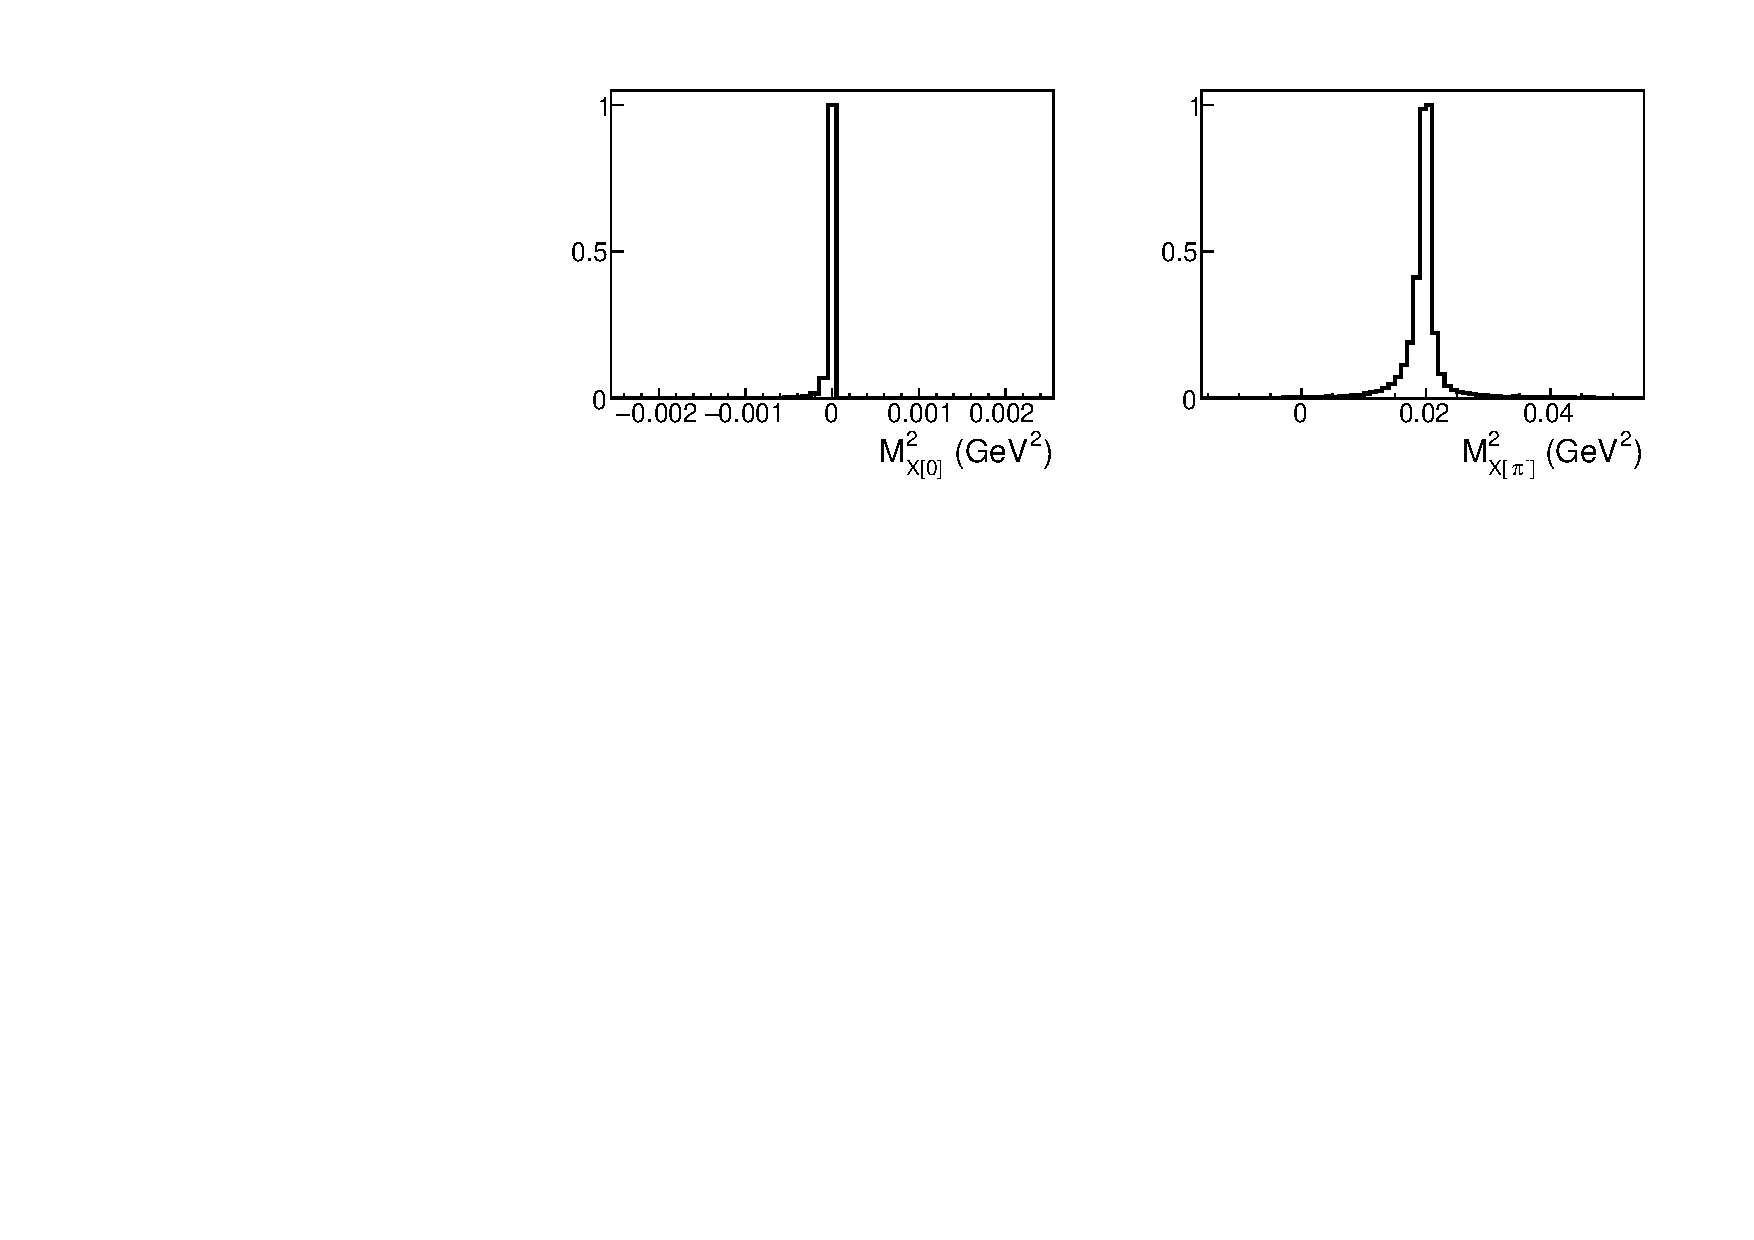
\includegraphics[width=0.8\textwidth]{pictures/appendix/mm_res.pdf}}
\caption{\small Impact of the detector resolution on $M_{X[0]}^{2}$ (left) and $M_{X[\pi^{-}]}^{2}$ (right). The distribution of $M_{X[0]}^{2}$ is zoomed in on $x$ to demonstrate the disturbances.} \label{fig:mm_res}
\end{center}
\end{figure}
\vspace{-1.5em}

This impact of the detector resolution\footnote[4]{To produce this plot, generated events were reconstructed via CLAS reconstruction software.} on $M_{X[0]}^{2}$ and $M_{X[\pi^{-}]}^{2}$ is demonstrated in Fig.~\ref{fig:mm_res}, where $M_{X[0]}^{2}$ is shown to be visually very narrow with slight disturbances, while $M_{X[\pi^{-}]}^{2}$ acquires perceptible smearing. 


\vspace{-0.75em}
\subsection*{Final state interactions}
\vspace{-0.5em}
Let's estimate the quantities $M_{X[0]}^{2}$ and $M_{X[\pi^{-}]}^{2}$ considering the change of the final hadron momenta as in the case of FSI. To simplify the estimation, let's assume the following: (i) for each event only one final state hadron is affected\footnote[5]{This imitates the interaction with the remaining neutron for the case of deuteron target.}, (ii) the type of the affected hadron is the same among all events in the sample, (iii) FSI are limited to the change of the momentum magnitude of the affected hadron as $p'_{h} = \varepsilon p_{h}$, and (iv) such momentum modification occurs in all events in the sample. Then\vspace{-0.5em}
\begin{equation}
\begin{aligned}
&M_{X[0]}^{2}&=&~[P^{\mu}_{h} -P'^{\mu}_{h}]^{2} = [P^{\mu}_{h}]^{2} +[P'^{\mu}_{h}]^{2}-2(P^{\mu}_{h}\cdot P'^{\mu}_{h} )=\\
&&=&~2m^{2}-2(EE' - (\overrightarrow{p}\cdot \overrightarrow{p}'))=\\
&&=&~2m^{2} - 2(\sqrt{m^{2}+p^{2}}\sqrt{m^{2}+\varepsilon^{2}p^{2}}-\varepsilon p^{2}),\\[-7pt]
\end{aligned}\label{eq:mm0_fsi}
\end{equation}
where $m$ and $p$ are the mass and the momentum magnitude of the affected hadron.


The final expression in Eq.~\eqref{eq:mm0_fsi} is always less than zero regardless of both the value of $\varepsilon$ and hadron kinematics, as the comparison below demonstrates.\vspace{-0.5em}
\begin{equation}
\begin{aligned}
2m^{2} - 2(\sqrt{m^{2}+p^{2}}\sqrt{m^{2}+\varepsilon^{2}p^{2}}-\varepsilon p^{2})& ~~\wedge~~ 0&\\
m^{2} - \sqrt{m^{2}+p^{2}}\sqrt{m^{2}+\varepsilon^{2}p^{2}} +\varepsilon p^{2} &~~\wedge~~ 0&\\
m^{2}+\varepsilon p^{2} &~~\wedge~~ \sqrt{m^{2}+p^{2}}\sqrt{m^{2}+\varepsilon^{2}p^{2}}&\\
m^{4}+\varepsilon^{2}p^{4}+2m^{2}\varepsilon p^{2} &~~\wedge~~ m^{4} + p^{2}m^{2} + m^{2}\varepsilon^{2}p^{2}+\varepsilon^{2}p^{4}&\\
2m^{2}\varepsilon p^{2} &~~\wedge~~ p^{2}m^{2}+  m^{2}\varepsilon^{2}p^{2}&\\
0 &~~\wedge~~ p^{2}m^{2}(\varepsilon^{2}-2\varepsilon+1)&\\
0&~~<~~ p^{2}m^{2}(\varepsilon-1)^{2}&\\[-7pt]
\end{aligned}\label{eq:comp}
\end{equation}
\vspace{-0.3em}
The quantity $M_{X[\pi^{-}]}^{2}$ in turn can be written as\vspace{-0.5em}
\begin{equation}
\begin{aligned}
&M_{X[\pi^{-}]}^{2}&=&~[P^{\mu}_{\pi^{-}}+ P^{\mu}_{h} -P'^{\mu}_{h}]^{2} =\\
&&=&~[P^{\mu}_{\pi^{-}}]^{2} +[P^{\mu}_{h} -P'^{\mu}_{h}]^{2}+2P^{\mu}_{\pi^{-}}(P^{\mu}_{h} -P'^{\mu}_{h})= \\
&&=&~m_{\pi}^{2} + M_{X[0]}^{2} +2\left \{E_{\pi^{-}}(E_{h}-E'_{h}) - (\overrightarrow{p}_{\pi^{-}}\cdot \overrightarrow{p}_{h})(1-\varepsilon)\right \},\\[-7pt]
\end{aligned}\label{eq:rrr}
\end{equation}
which can be either greater or smaller than zero depending on the value of $\varepsilon$ and kinematics.

\begin{figure}[htp]
\begin{center}
\framebox{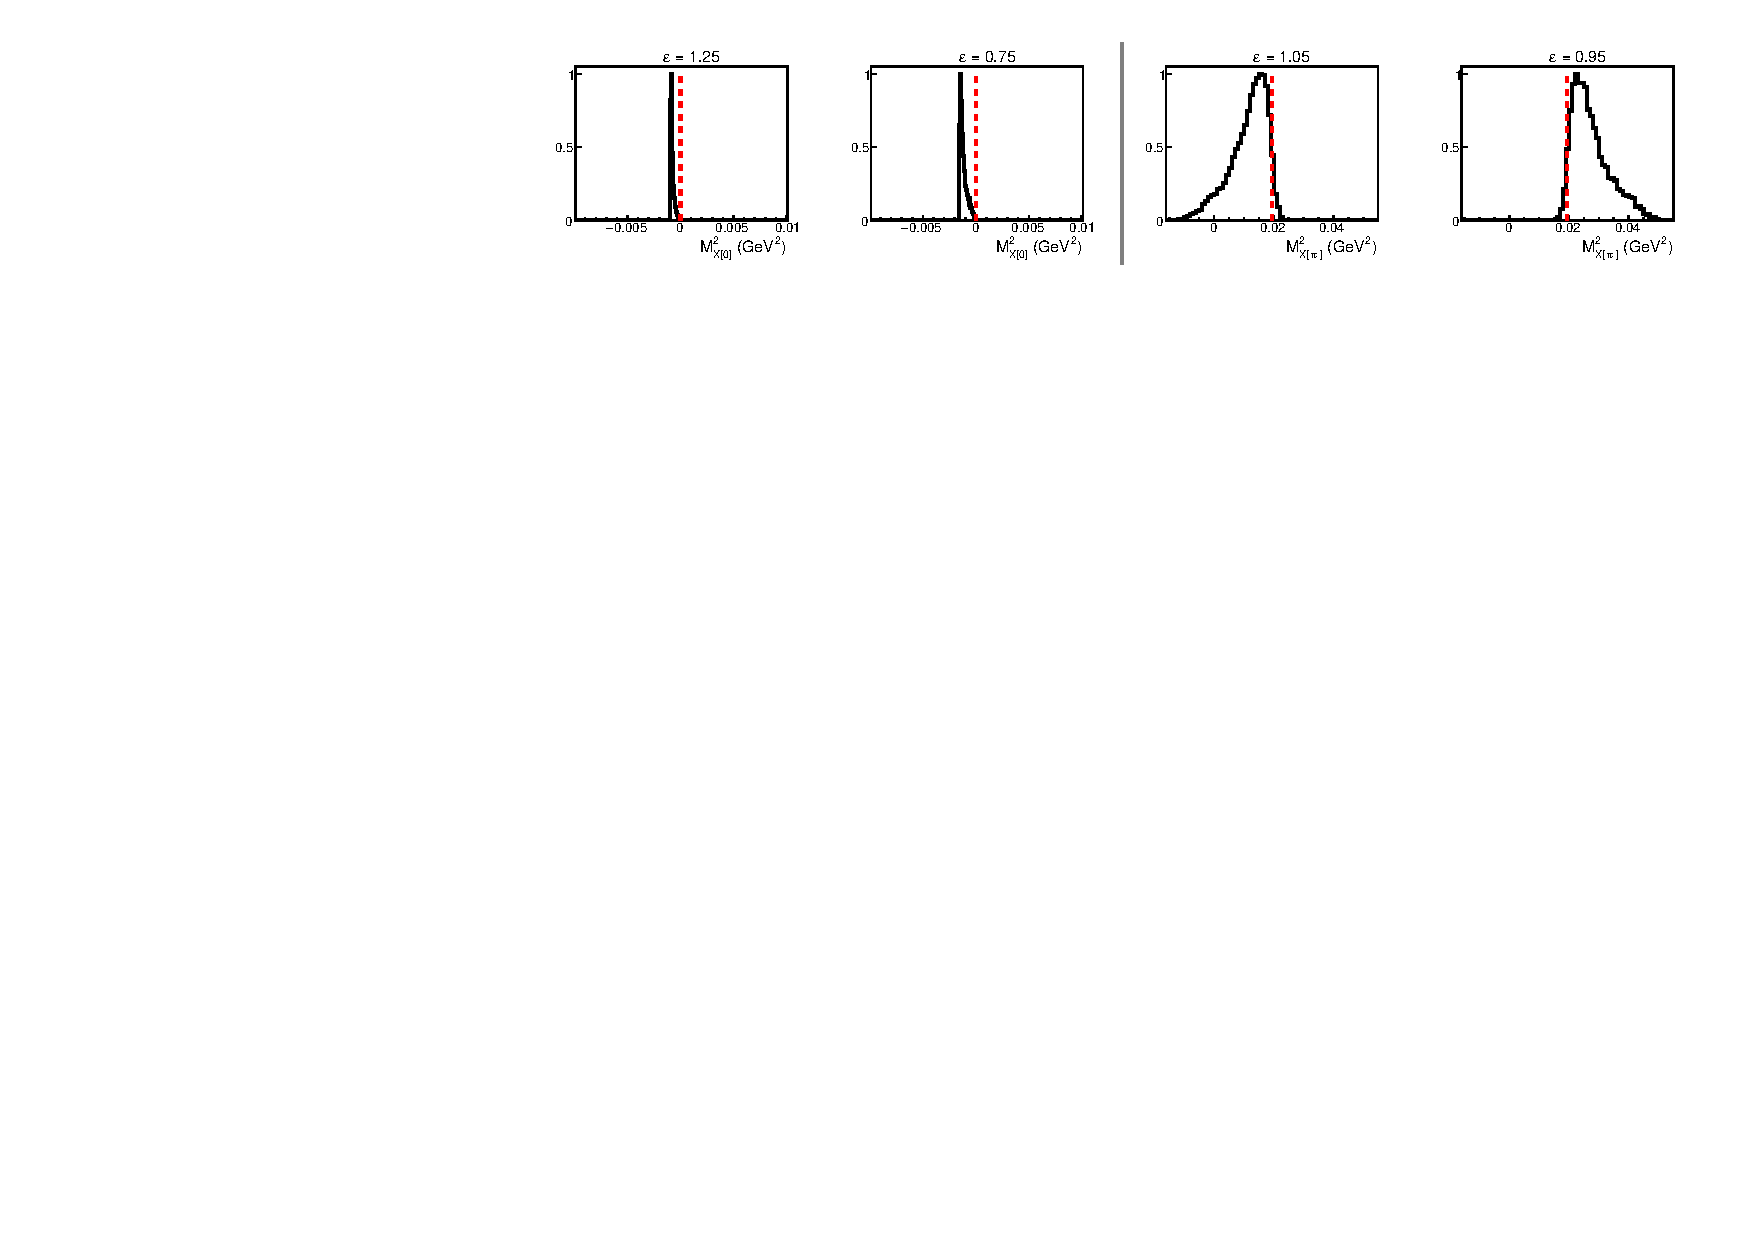
\includegraphics[width=\textwidth]{pictures/appendix/mm_pip_fsi.pdf}}
\caption{\small Quantities $M_{X[0]}^{2}$ (left side) and $M_{X[\pi^{-}]}^{2}$ (right side) plotted assuming the change of the $\pi^{+}$ momentum magnitude as $p'_{\pi^{+}} = \varepsilon p_{\pi^{+}}$. Red dashed lines mark the position of zero and pion mass squared, respectively.  } \label{fig:mm_pip_fsi}
\end{center}
\end{figure}
\vspace{-1.5em}

\begin{figure}[htp]
\begin{center}
\framebox{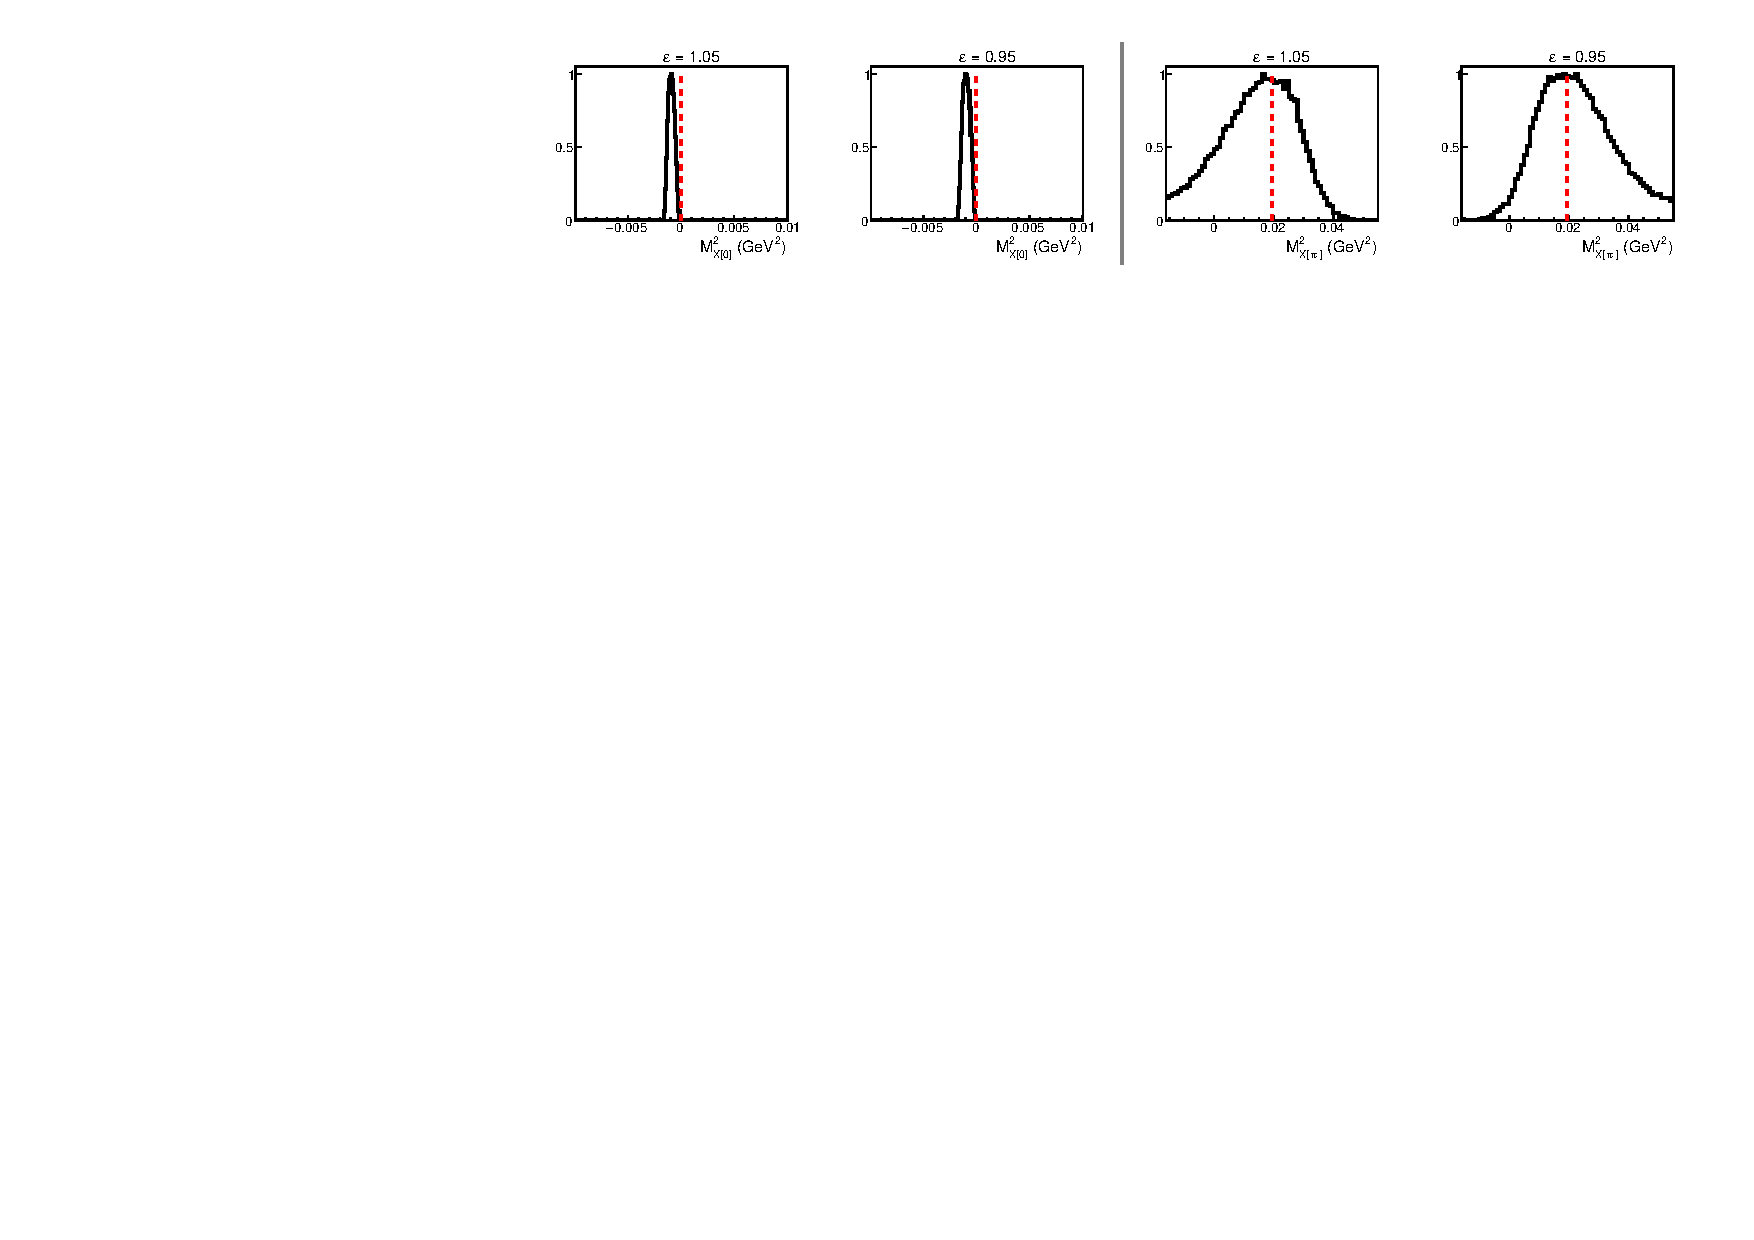
\includegraphics[width=\textwidth]{pictures/appendix/mm_pr_fsi.pdf}}
\caption{\small Quantities $M_{X[0]}^{2}$ (left side) and $M_{X[\pi^{-}]}^{2}$ (right side) plotted assuming the change of the momentum magnitude of the final proton as $p'_{p'} = \varepsilon p_{p'}$. Red dashed lines mark the position of zero and pion mass squared, respectively. } \label{fig:mm_pr_fsi}
\end{center}
\end{figure}
\vspace{-1.5em}

Figure~\ref{fig:mm_pip_fsi} shows the distributions of $M_{X[0]}^{2}$ and $M_{X[\pi^{-}]}^{2}$ for the case, when all positive pions change their momenta as $p'_{\pi^{+}} = \varepsilon p_{\pi^{+}}$. The quantity $M_{X[0]}^{2}$ (left side) is plotted for the sizable values of $\varepsilon$ ($\varepsilon = 1.25$ and $\varepsilon = 0.75$), since it turns out to be rather insensitive to the change of pion momenta. The quantity 
$M_{X[\pi^{-}]}^{2}$ (right side), being in contrast rather sensitive to the $\pi^{+}$ momentum change, is plotted for $\varepsilon = 1.05$ and $\varepsilon = 0.95$.

Figure~\ref{fig:mm_pr_fsi} shows the distributions of $M_{X[0]}^{2}$ and $M_{X[\pi^{-}]}^{2}$ for the case, when all final protons change their momenta as $p'_{p'} = \varepsilon p_{p'}$. Both $M_{X[0]}^{2}$ (left side) and $M_{X[\pi^{-}]}^{2}$ (right side) turn out to be sensitive to the proton momentum change and therefore are plotted for $\varepsilon = 1.05$ and $\varepsilon = 0.95$.

%\clearpage
%\end{comment}
%========================================================================
%\newpage
\renewcommand{\thesection}{B}
 \refstepcounter{section}
    \makeatletter
   \renewcommand{\theequation}{\thesection.\@arabic\c@equation}
    \makeatother
\section*{Appendix B: Lab to CMS transformation for the proton at rest case}
\label{app_lab_cms_trans}
\addcontentsline{toc}{section}{B: Lab to CMS transformation for the case of proton at rest}

Here the procedure of the Lab to CMS transformation for an electroproduction experiment off the proton at rest (bottom left illustration in Fig.~\ref{fig:lab_to_CMS}) is described~\cite{Fed_an_note:2017}. In this case the CMS axis orientation is different for each reaction event and is specified by the direction of the scattered electron. The transformation from Lab to CMS includes the following steps\footnote[1]{In all derivations the energy is assumed to be the last component of the four-momentum and the four-momentum to be a row vector.}:\vspace{-1em}

\begin{enumerate}
\item The $xy$-plane of the Lab system is rotated around the $z$-axis (given by the incoming electron direction) to make the $x$-axis lying in the electron scattering plane (see Fig.~\ref{fig:cr_sec_el_angles}). This rotation transforms the four-momentum as $P' = P \cdot R_1(\varphi_{e'})$, with 

\begin{equation}
R_{1}(\varphi_{e'}) = \begin{pmatrix}
 \cos\varphi_{e'}& -\sin\varphi_{e'} & 0 &0 \\ 
 \sin\varphi_{e'}& \cos\varphi_{e'} &  0& 0\\ 
0 & 0 & 1 &0 \\ 
 0&  0&  0&1 
\end{pmatrix},
\end{equation}
where $\varphi_{e'}$ is the azimuthal angle of the scattered electron.

\begin{figure}[htp]
\begin{center}
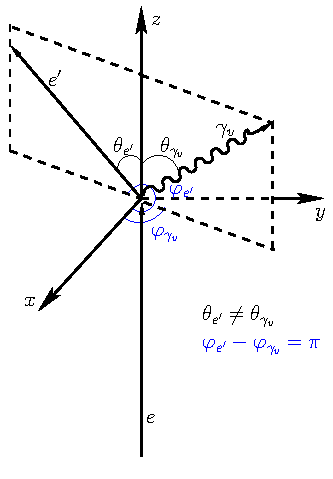
\includegraphics[width=5.8cm]{pictures/appendix/electron_angles.pdf}
\caption{\small Virtual photon and scattered electron angles $\theta$ and $\varphi$ in the Lab frame for the proton at rest experiment.} \label{fig:cr_sec_el_angles}
\end{center}
\end{figure}

%\vspace{-1em}
After this rotation $\varphi_{e'} = 0$, while $\varphi_{\gamma_v} = \pi$ with respect to the intermediate reference frame.

\item The Lab system is then rotated to align the $z$-axis with the virtual photon direction. The four-momentum transformation for this rotation is given by $P'' = P' \cdot R_2 (\theta_{\gamma_{v}})$, with 
\begin{equation}
R_{2}(\theta_{\gamma_{v}})=\begin{pmatrix}
\cos\theta_{\gamma_{v}} &0  &-\sin\theta_{\gamma_{v}}  &0 \\ 
 0& 1 & 0 &0 \\ 
 \sin\theta_{\gamma_{v}} &0  &\cos\theta_{\gamma_{v}}  & 0\\ 
0 &0  & 0 &1 
\end{pmatrix},
\end{equation}
where $\theta_{\gamma_v}$ is the polar angle of the virtual photon\footnote[2]{Using embedded ROOT functions, both rotations can be coded using the unit vectors TVector3~$uz$~=~P4\_gamma.Vect().Unit() and 
 TVector3~$ux$~=~(P4\_EL.Vect().Cross(P4\_ELP.Vect())).Unit(), where P4\_gamma, P4\_EL, and P4\_ELP are the four-momenta of the virtual photon, initial and final electrons, respectively. 
 The axis vector $ux$ needs to be rotated according to $ux$.Rotate(3.*M\_PI/2,$uz$).
Finally the rotation is defined as rot.SetZAxis($uz$,$ux$).Invert() and needs to be applied to the four-momentum (P4) of each particle:
 P4.Transform(rot).}.

\item Finally, a boost into the CM frame of the {\em virtual photon -- initial proton} system is performed. It is given by the formula $P''' = P'' \cdot R_3(\beta)$, with 
\begin{equation}
R_{3}(\beta) = \begin{pmatrix}
1 &0  &0  &0 \\ 
0 &1  &0  &0 \\ 
 0&  0& \gamma  &-\gamma \beta  \\ 
 0&  0& -\gamma \beta  & \gamma 
\end{pmatrix}, \, \, \, \beta =\frac{|\overrightarrow{q}|}{E_{\gamma }+m_{proton}}=\frac{\sqrt{E^{2}_{\gamma }+Q^{2}}}{E_{\gamma }+m_{proton}}, \, \, \,\,  \gamma =\frac{1}{\sqrt{1-\beta ^{2}}},
\end{equation}
where $|\overrightarrow{q}|$ is the magnitude of the three-vector of the virtual photon and $\beta$ the magnitude and $z$-component of the three-vector\footnote[3]{
Note: if you use the ROOT function .Boost, you should change the sign of the $z$-component of $\beta$-vector as .Boost(0,0,-$\beta$).} $\overrightarrow{\beta}=(0,0,\beta)$.
\end{enumerate}


%================================================

\renewcommand{\thesection}{C}
 \refstepcounter{section}
    \makeatletter
   \renewcommand{\theequation}{\thesection.\@arabic\c@equation}
    \makeatother
\section*{Appendix C: The reaction phase-space}
\label{app_ph_space}
\addcontentsline{toc}{section}{C: The reaction phase-space}



The phase-space of the reaction $ep \rightarrow e'p'\pi^{+}\pi^{-}$ is determined by seven kinematic variables, i.e. $W$, $Q^{2}$, $M_{h_{1}h_{2}}$, $M_{h_{2}h_{3}}$, $\theta_{h_{1}}$, $\varphi_{h_{1}}$, and $\alpha_{h_{1}}$ (see Sect.~\ref{Sect:kin_var} for details). The kinematic coverage for various variables has the following specificities.\vspace{-0.2em} 
\begin{itemize}
\item In the $W$ and $Q^{2}$ variables it depends on the electron beam energy and experimental conditions and is fixed for a particular experiment. \vspace{-0.3em}
\item The angular variables $\theta_{h_{1}}$, $\varphi_{h1}$, and $\alpha_{h1}$ vary in the fixed limits of $[0,~\pi]$, $[0,~2\pi]$, and $[0,~2\pi]$, respectively.\vspace{-0.3em}
\item In the invariant masses $M_{h_{1}h_{2}}$ and $M_{h_{2}h_{3}}$ the coverage depends on $W$ and broadens as $W$ grows.\vspace{-0.2em}
\end{itemize}
\vspace{-1em}
\begin{figure}[htp]
\begin{center}
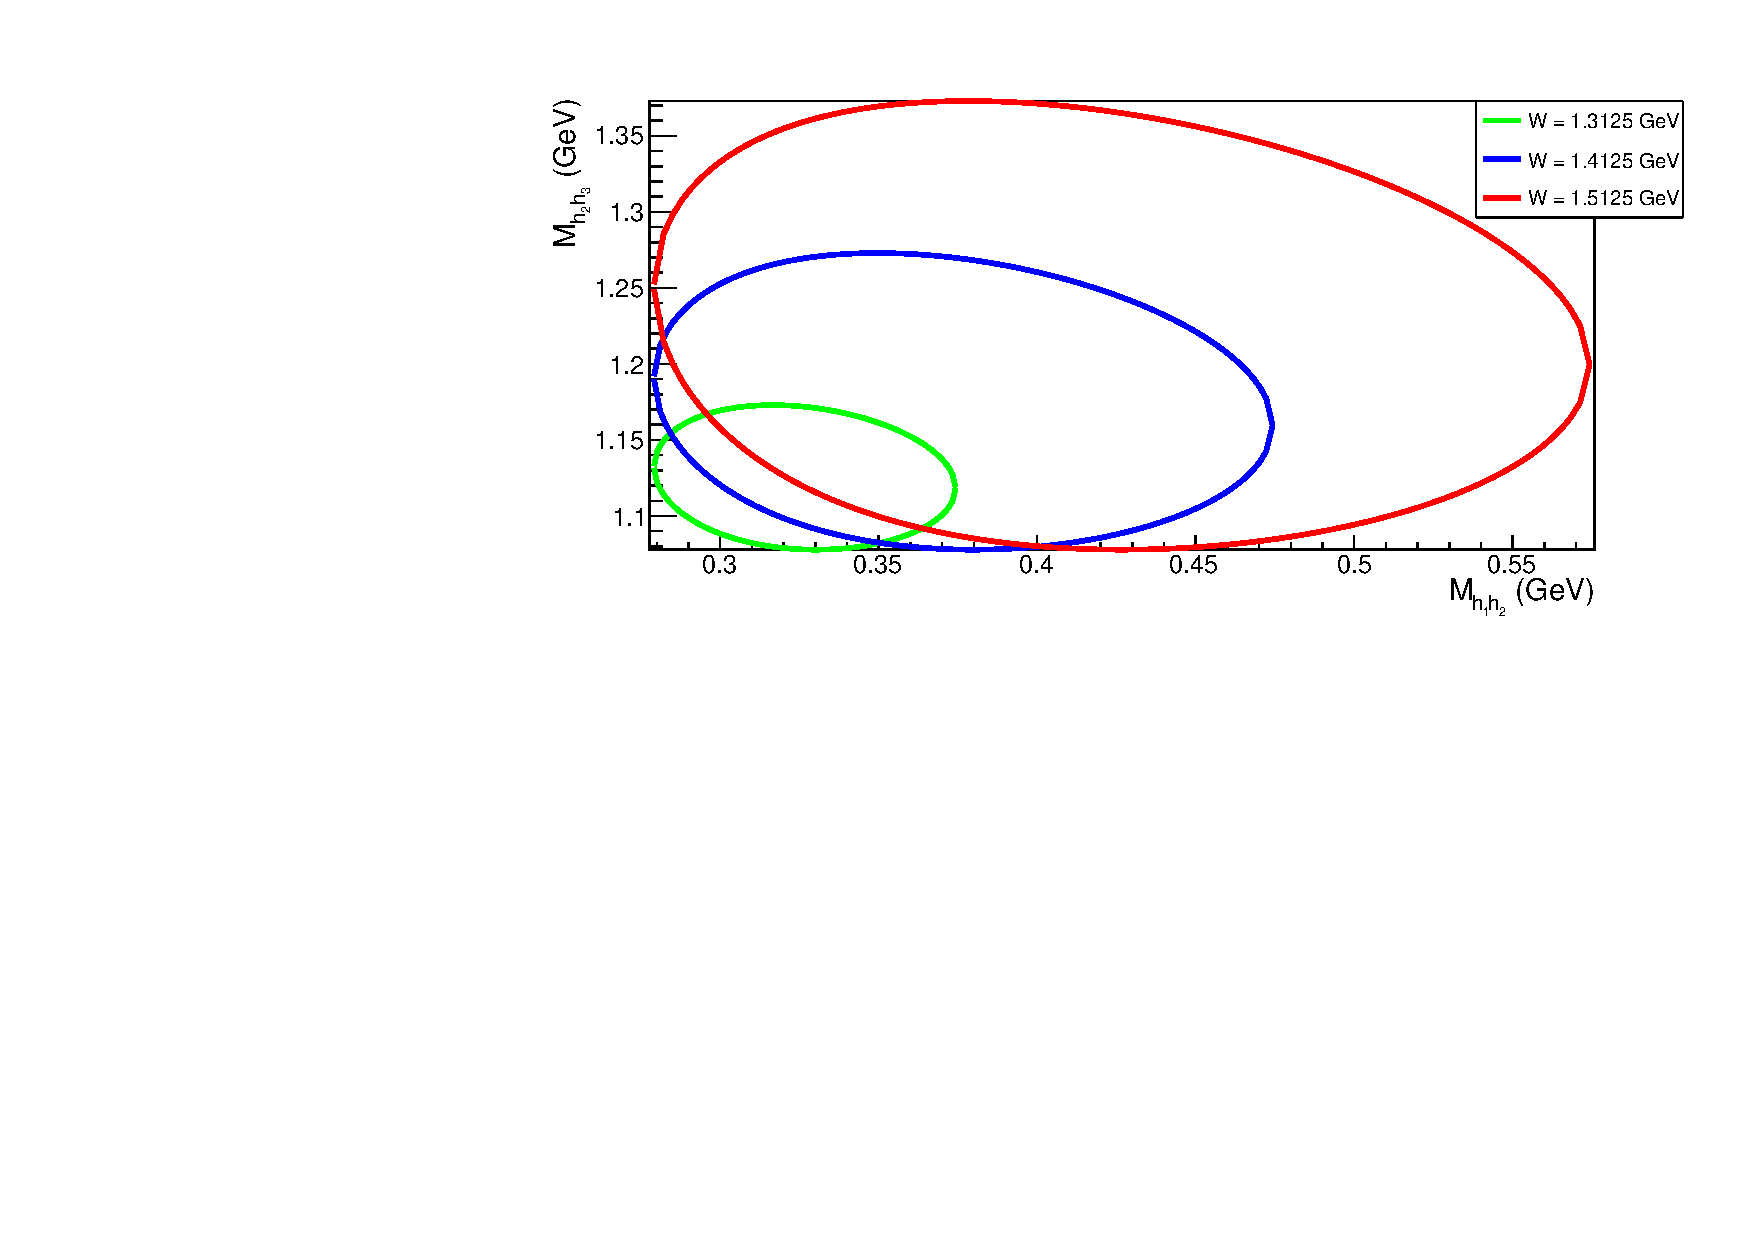
\includegraphics[width=13cm]{pictures/appendix/dalitz_plots_boundaries.pdf}
\caption{\small Boundary of the $M_{h_{2}h_{3}}$ versus $M_{h_{1}h_{2}}$ distribution for several distinct values of $W$ specified in the plot.} \label{fig:dalitz}
\end{center}
\end{figure}

The shape of the reaction phase-space in the invariant masses is determined by the condition $B(M_{h_{1}h_{2}}^{2}, M_{h_{2}h_{3}}^{2}, W^{2}, m_{h_{2}}^{2}, m_{h_{1}}^{2}, m_{h_{3}}^{2}) = 0$, where $B(x, y, z, u, v, w)$ is the Byckling function~\cite{Byckling:1971vca} given by 
\begin{equation}
\begin{split}
B(x,y,z,u,v,w) = &x^{2}y+xy^{2}+z^{2}u+zu^{2}+v^{2}w+vw^{2}+ \\   
&xzw+xuv+yzv+yuw- xy(z+u+v+w)- \\ 
&zu(x+y+v+w)-vw(x+y+z+u).
\label{eq:byckling}
\end{split}
\end{equation}

Figure~\ref{fig:dalitz} shows the boundary of the $M_{h_{2}h_{3}}$ versus $M_{h_{1}h_{2}}$ distribution for several values of $W$ specified in the plot and visually demonstrates the effect  of the phase-space broadening with the increase of $W$.


%============================================

%\begin{comment}
\renewcommand{\thesection}{D}
 \refstepcounter{section}
    \makeatletter
   \renewcommand{\theequation}{\thesection.\@arabic\c@equation}
    \makeatother
\section*{Appendix D: Uncertainties for indirect measurements}
\label{app_uncert}
\addcontentsline{toc}{section}{D: Uncertainties for indirect measurements}



Some useful examples of the error propagation for indirect measurements are described here. In these examples one assumes that $a>0$, $b>0$, and $c>0$.



\begin{itemize}

\item If independent variables $x_{1}$ and $x_{2}$ have absolute uncertainties $\Delta x_{1}$ and $\Delta x_{2}$, respectively, then the absolute uncertainty of the variable $y=c(\frac{x_{1}}{a} - \frac{x_{2}}{b})$ is

\begin{equation}
\begin{aligned}
\Delta y = c\sqrt{\left (\frac{ \Delta x_{1}}{a} \right )^{2} + \left (\frac{ \Delta x_{2}}{b} \right )^{2}}.
\label{eq:err_subtr}
\end{aligned}
\end{equation}


\item If the variable $x$ has an absolute uncertainty $\Delta x$, then the absolute uncertainty of the variable $y=\frac{a}{x}$ is

\begin{equation}
\begin{aligned}
\Delta y = \frac{a}{x^{2}}\cdot \Delta x = y\cdot \frac{\Delta x}{x}.
\label{eq:err_frac}
\end{aligned}
\end{equation}


\item If the variable $x$ has an absolute uncertainty $\Delta x$, then the absolute uncertainty of the variable $y=\frac{a\cdot x +b}{c}$ is

\begin{equation}
\begin{aligned}
\Delta y = \frac{a\cdot \Delta x}{c}.
\label{eq:err_prod}
\end{aligned}
\end{equation}



\item If there is a set of measurements $x_{1}$, $x_{2}$, ..., $x_{n}$ with the arithmetic mean $\overline{x}$, then the absolute standard error of the arithmetic mean is

 
\begin{equation}
\begin{aligned}
\Delta \overline{x} = \sqrt{\frac{\sum\limits_{i=1}^{n} (x_{i}-\overline{x})^{2}}{n\cdot(n-1)}}.
\label{eq:err_arith_mean}
\end{aligned}
\end{equation}

\end{itemize}



%==========================================
\newpage

\renewcommand{\thesection}{E}
 \refstepcounter{section}
    \makeatletter
   \renewcommand{\theequation}{\thesection.\@arabic\c@equation}
    \makeatother
\section*{Appendix E: Analysis procedure and code availability}
\label{app_code}
\addcontentsline{toc}{section}{E: Analysis procedure and code availability}

The following files are used as an input for the analysis.\vspace{-1em}

\begin{itemize}
\item 1989 files with full target runs stored at\\[-0.75mm]
 /mss/clas/e1e/production/pass1/h10/\vspace{-0.7em}
\item 14 files with empty target runs stored at\\[-0.75mm]
/mss/clas/e1e/production/pass1/h10\_emptarg\_d/\vspace{-0.7em}
\item 165625 files with the Monte Carlo simulation. They are stored at\\[-0.75mm]
/mss/clas/e1e/production/simulation\_2pi/sim\_skorodum\_Aug2016/nt10*
\vspace{-0.5em}
\end{itemize}


All these files contain ``h10" ROOT ntuples. They were converted from HBOOK outputs of nt10maker (which is a part of CLAS software) using the ``h2root" utility.

The scripts used for performing the Monte Carlo simulation, which incorporate the information on the simulation/reconstruction parameters used in this analysis, can be found here {\bf https://github.com/skorodumina/CLAS6\_sim\_rec\_sequence}.


To speed up the analysis process, the specified above files are converted to reduced ``t21" ROOT ntuples, which contain only those variables that are used in the analysis (the conversion program is available at {\bf https://github.com/skorodumina/converter\_clas6.git}). After the conversion one is left with \vspace{-1em}

\begin{itemize}
\item 284 files with full target runs stored at\\[-0.75mm] 
/mss/home/skorodum/e1e/data\_2pi\_conv\_2July2018/\vspace{-0.7em}
\item 1 file with empty target runs, i.e.\\[-0.75mm]
/mss/home/skorodum/e1e/out\_conv\_empty\_2pi\_2July2018.root \vspace{-0.7em}
\item 33125 files with the simulation. They are stored at /mss/clas/e1e/production/\\[-0.75mm]
simulation\_2pi/sim\_skorodum\_Aug2016/converted\_July2018\_cc\_ok/
\vspace{-0.5em}
\end{itemize}


For further calculations the double-pion analysis program is used (it is available at {\bf https://github.com/skorodumina/two\_pi\_analysis\_code.git}). This program outputs the root file with multi-dimensional histograms.

For the experimental data this process is rather simple:\vspace{-1em}

\begin{itemize}

\item 284 full target files are fed to the double-pion analysis program at once. \vspace{-0.7em}
\item 1 empty target file is fed to the same program. \vspace{-0.7em}
\item Both outputs for full and empty target runs are processed with the corresponding script to combine the topologies. This results in the output file $out\_data.root$. \vspace{-0.5em}

\end{itemize}



For the Monte Carlo simulation the process is more complicated.\vspace{-1em}

\begin{itemize}
\item 33125 files with the simulation are processed on batch farms with the double-pion analysis program to produce 1325 output files with multi-dimensional histograms.\vspace{-0.7em}

\item These 1325 files are then processed with the corresponding scripts. As a result one has three sets of 53 files each. Files within each set contain multi-dimensional histograms filled with $\sigma$, $\sigma^{2}$, or 1.\vspace{-0.7em}

\item Then 53 files within each set are combined by the ROOT utility ``hadd" into three resulting files.\vspace{-0.7em}

\item The three files are processed with the corresponding scripts (which either combine topologies and/or calculate efficiency) with the three resulting outputs.\vspace{-0.7em}
\item These there outputs are combined (with ``hadd") to form the output $out\_sim.root$. \vspace{-0.5em}

\end{itemize}




Then the script that performs the cross section calculation is used. This script is located at {\bf https://github.com/skorodumina/twopi\_crsect\_calc.git} together with the aforementioned scripts. The program for unfolding the effects of the target motion is also located there (it is needed to produce the root file with the Fermi correction factor).

The script for the cross section calculation uses as inputs the files $out\_data.root$, $out\_sim.root$ and the file with the Fermi correction factor (all of them are introduced above). The script processes the multi-dimensional histograms from the input files and performs the cross section calculation that includes the empty target subtraction, normalization to the luminosity and the virtual photon flux, filling the empty cells, radiative corrections, and unfolding the effects of the initial proton motion. Beside this, the script also calculates the cross section uncertainty $\delta_{\text{stat,mod}}^{\text{tot}}$. The single-differential and integral cross sections are finally output to the root file.

Once the cross section is extracted, it is then subject to several final manipulations (i.e. binning corrections, averaging, and estimating the systematic uncertainties), which are performed by means of the corresponding scripts. They are also available at {\bf https://github.com/skorodumina/twopi\_crsect\_calc.git}.


The majority of codes introduced here are provided with their own README files, which are intended to clarify other details of the code performance.


%\end{comment}


\newpage

%==========================================

%\begin{comment}

\renewcommand{\thesection}{F}
 \refstepcounter{section}
    \makeatletter
   \renewcommand{\theequation}{\thesection.\@arabic\c@equation}
    \makeatother
\section*{Appendix F: Measured single-differential cross sections }
\label{app_cr_sect}
\addcontentsline{toc}{section}{F: Measured single-differential cross sections}

This Appendix contains the full set of single-differential cross sections measured in the current analysis. The cross sections are reported with the uncertainty $\delta_{\text{stat,mod}}^{\text{tot}}$ shown by error bars (see Sect.~\ref{Sect:mod_dep2}). The central point of the corresponding $W$ and $Q^{2}$ bin is specified in each figure together with the value of the relative integral systematic uncertainty (see Sect.~\ref{Sect:sys_uncert}) that can be propagated as a global factor to the corresponding single-differential cross sections.

Note that the invariant mass distributions are shown in the range from $M_{lower}$ to $M_{upper}$, both given by Eq.~\eqref{eq:inv_mass_boundary} with the latter calculated using the central value of the $W$ bin. One, therefore, should take into consideration that the cross section in invariant mass is equal to zero on both sides of the range. Also note that the invariant mass distributions contain one bin less than specified in Tab.~\ref{tab:summary_bins}, since the cross section in the last mass bins is not reported. This happens due to the special arrangement of mass bins used in the analysis, which forces the last bin to be situated out of the specified range (see Sect.~\ref{Sect:binning} for details).  


It is also noteworthy that $\alpha$ angular distributions of the double-pion cross sections should be symmetrical with respect to $\alpha = 180^{\rm o}$, when integrated over $\varphi$. However, the experimentally measured $\alpha$ distributions acquire some asymmetry. To judge more quantitatively the asymmetry degree, the average asymmetry factor was estimated for each extracted $\alpha$ distribution as
\begin{equation}
\begin{aligned}
\textrm{asym} = \frac{1}{\textrm{int} [ n/2]} \sum_{\substack{i = 1}}^{\substack{\textrm{int}[ n/2]}} \left | 1 - \frac{2\sigma_{i}}{\sigma_{i}+\sigma_{n-i}}\right |,
\label{eq:asym}
\end{aligned}
\end{equation}
where $n$ is the number of bins in the distribution and $\sigma_{i}$ the cross section value in the bin $i$.

The average asymmetry factor estimated by Eq.~\eqref{eq:asym} is specified in the plots for each $\alpha$ distribution to facilitate visual judgement of the distribution's shape and its inherent systematic inaccuracy.

\begin{figure}[htp]
\begin{center}
\frame{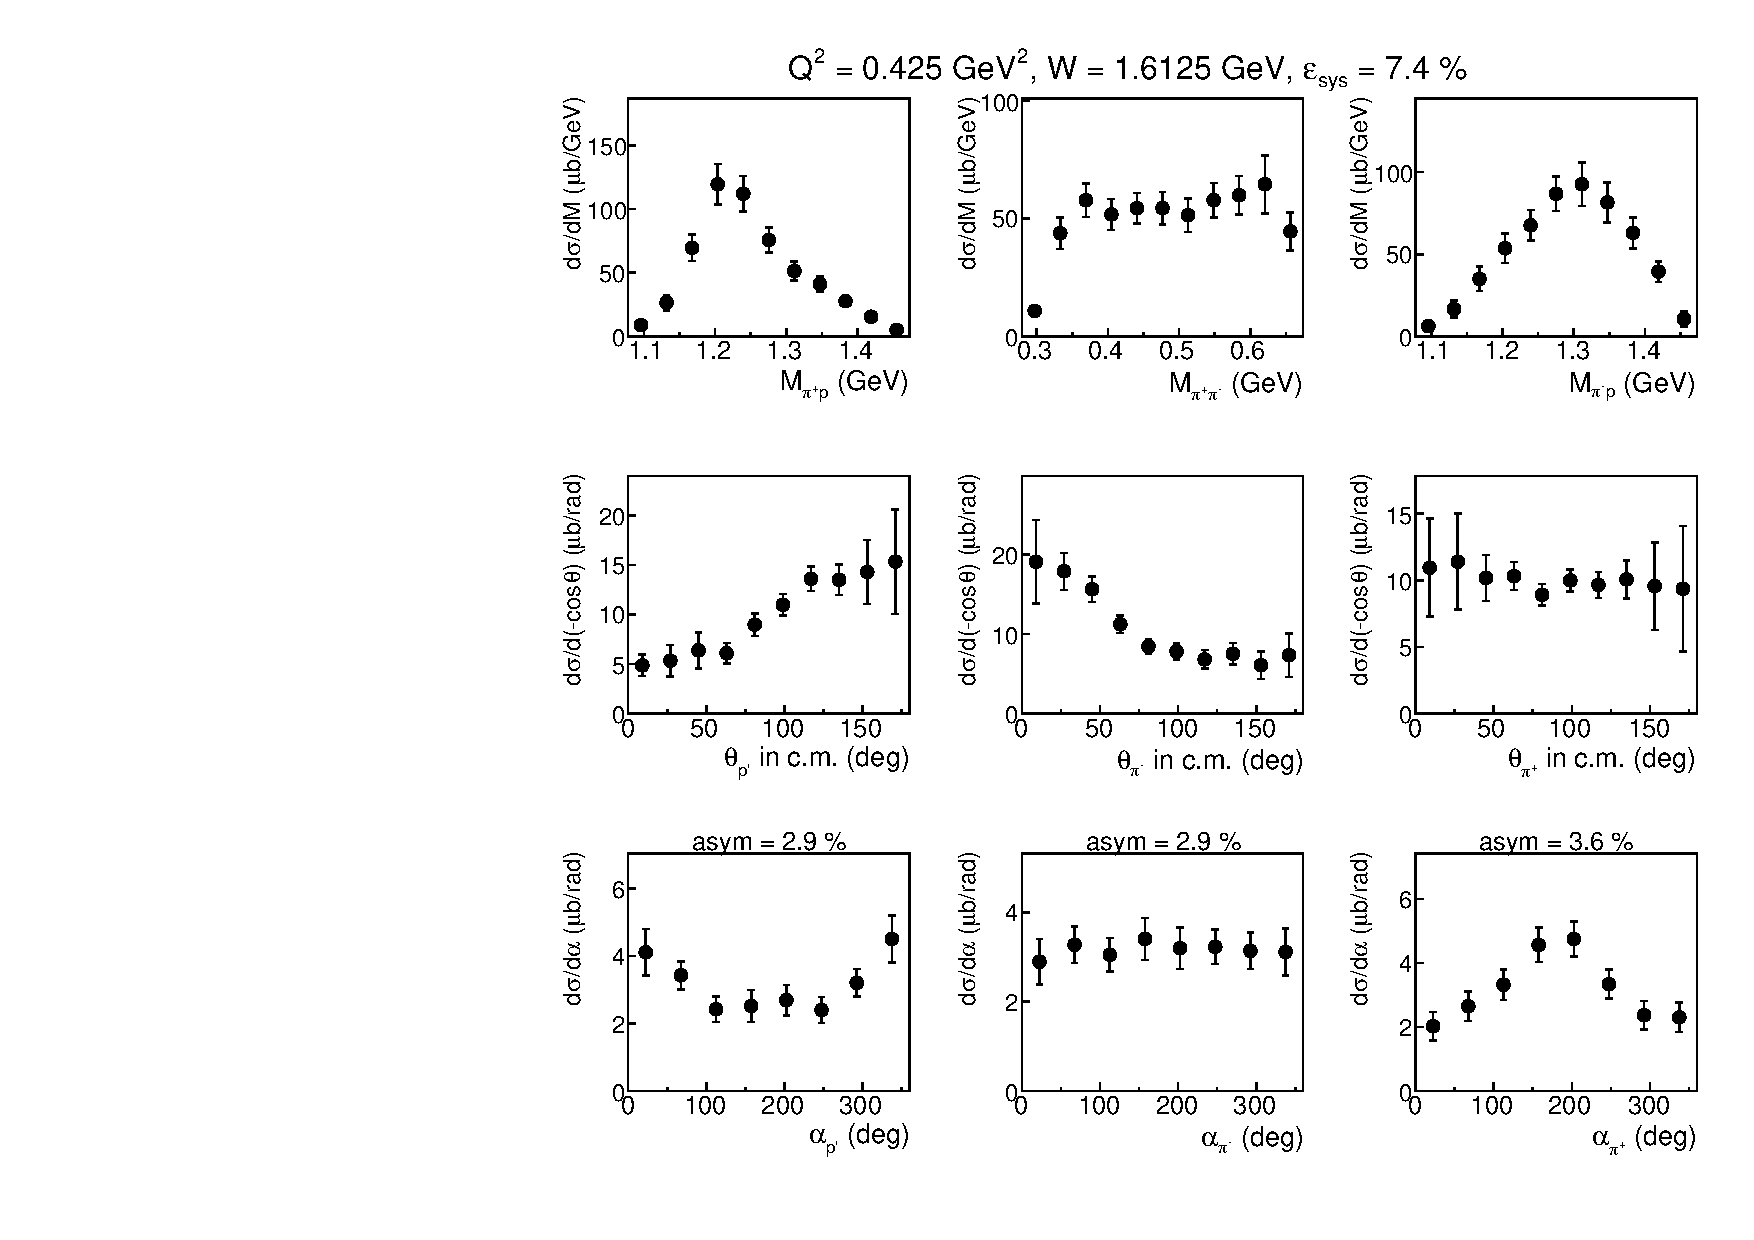
\includegraphics[width=0.45\textwidth]{pictures/appendix/1diff_distr/Q2_425/w_16125.pdf}}
\frame{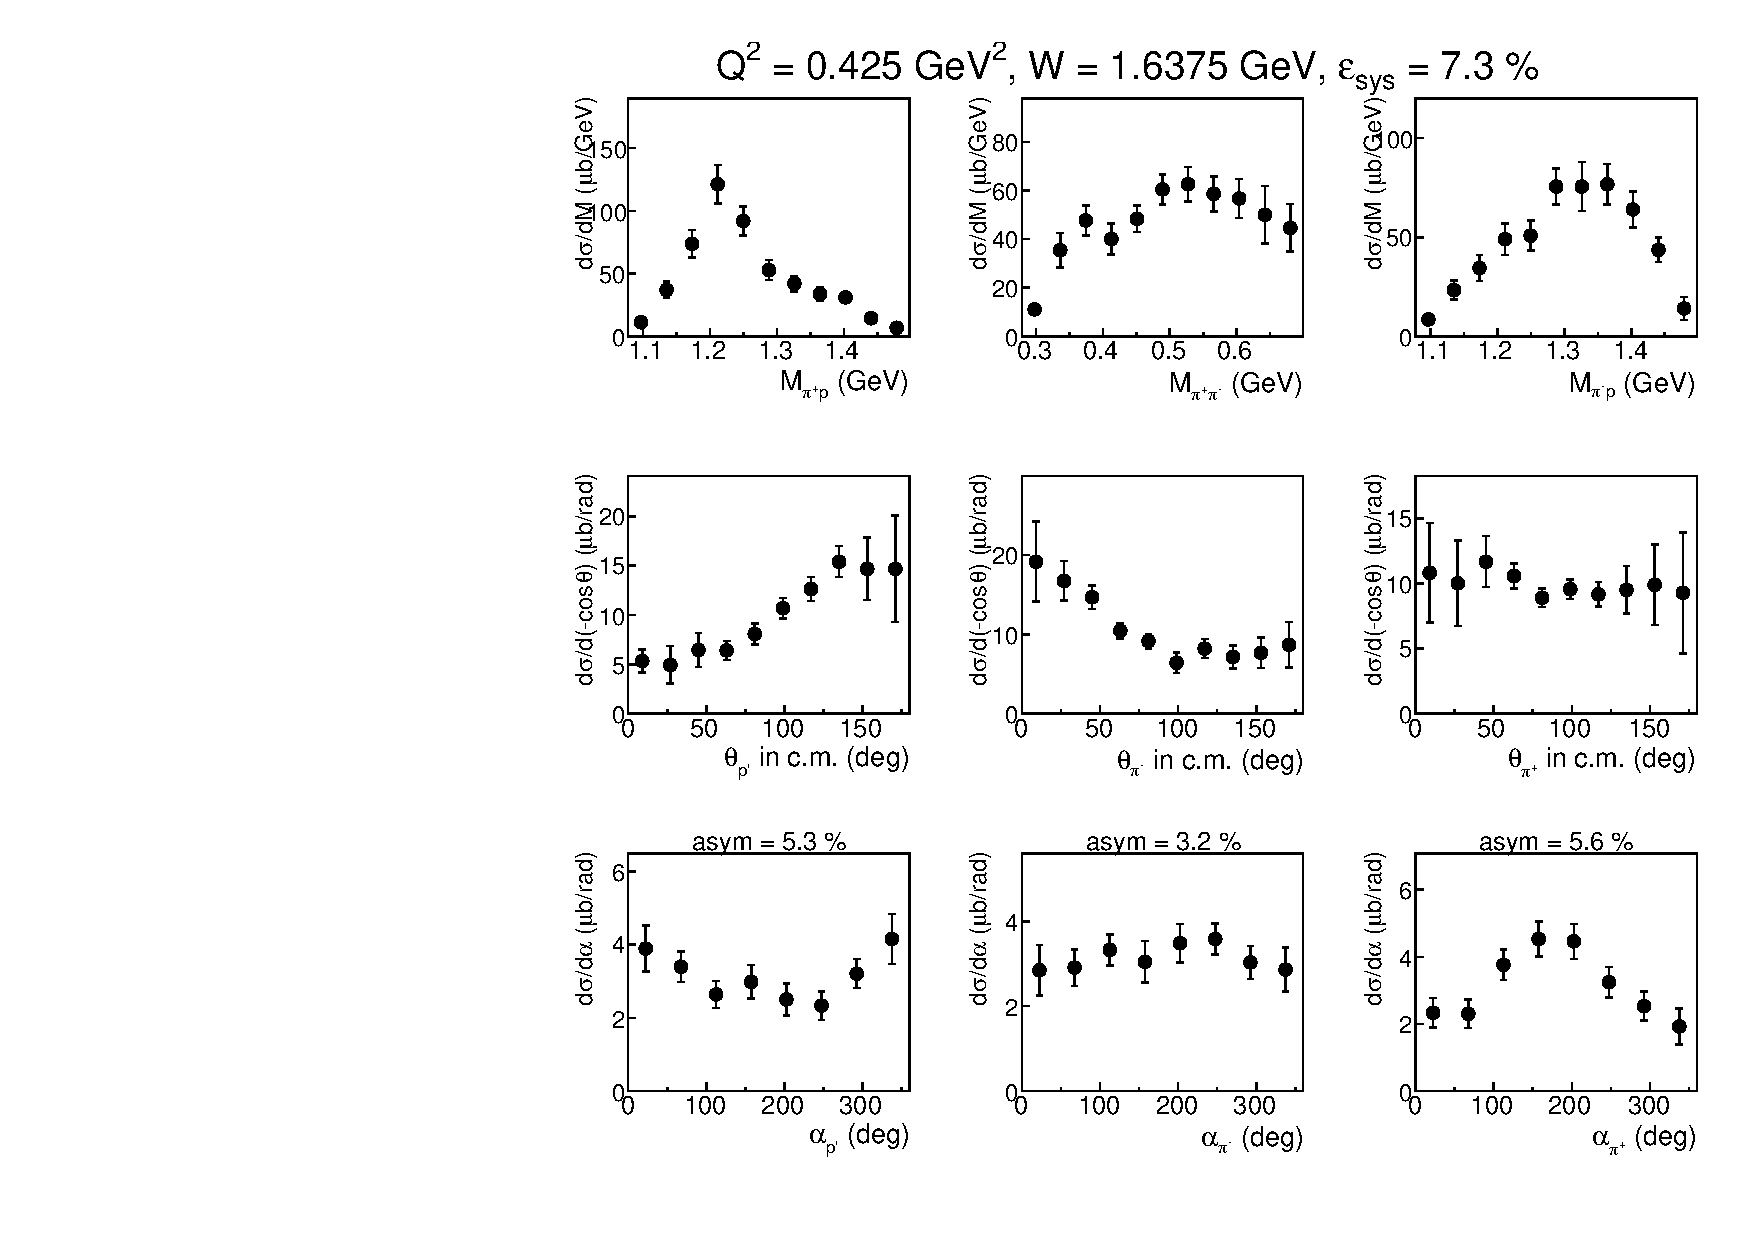
\includegraphics[width=0.45\textwidth]{pictures/appendix/1diff_distr/Q2_425/w_16375.pdf}}
\frame{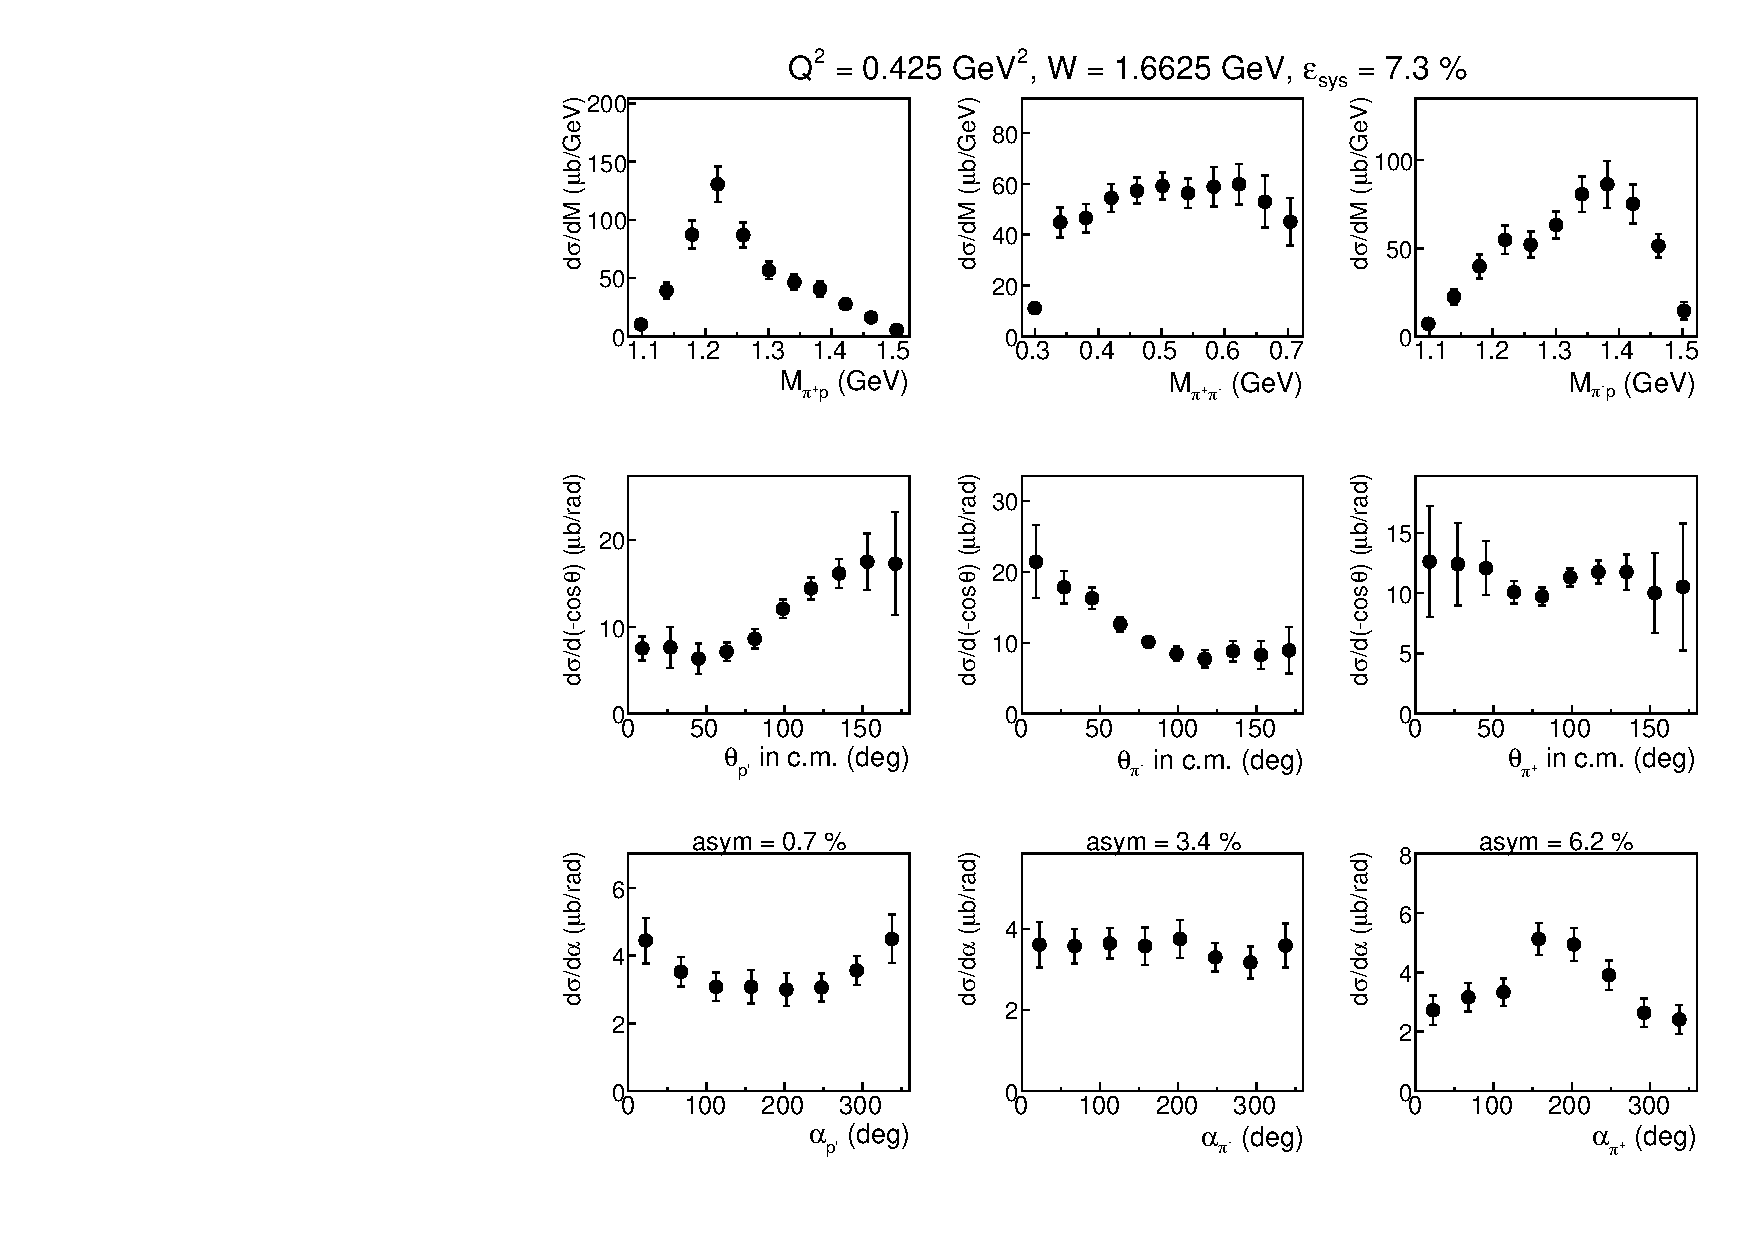
\includegraphics[width=0.45\textwidth]{pictures/appendix/1diff_distr/Q2_425/w_16625.pdf}}
\frame{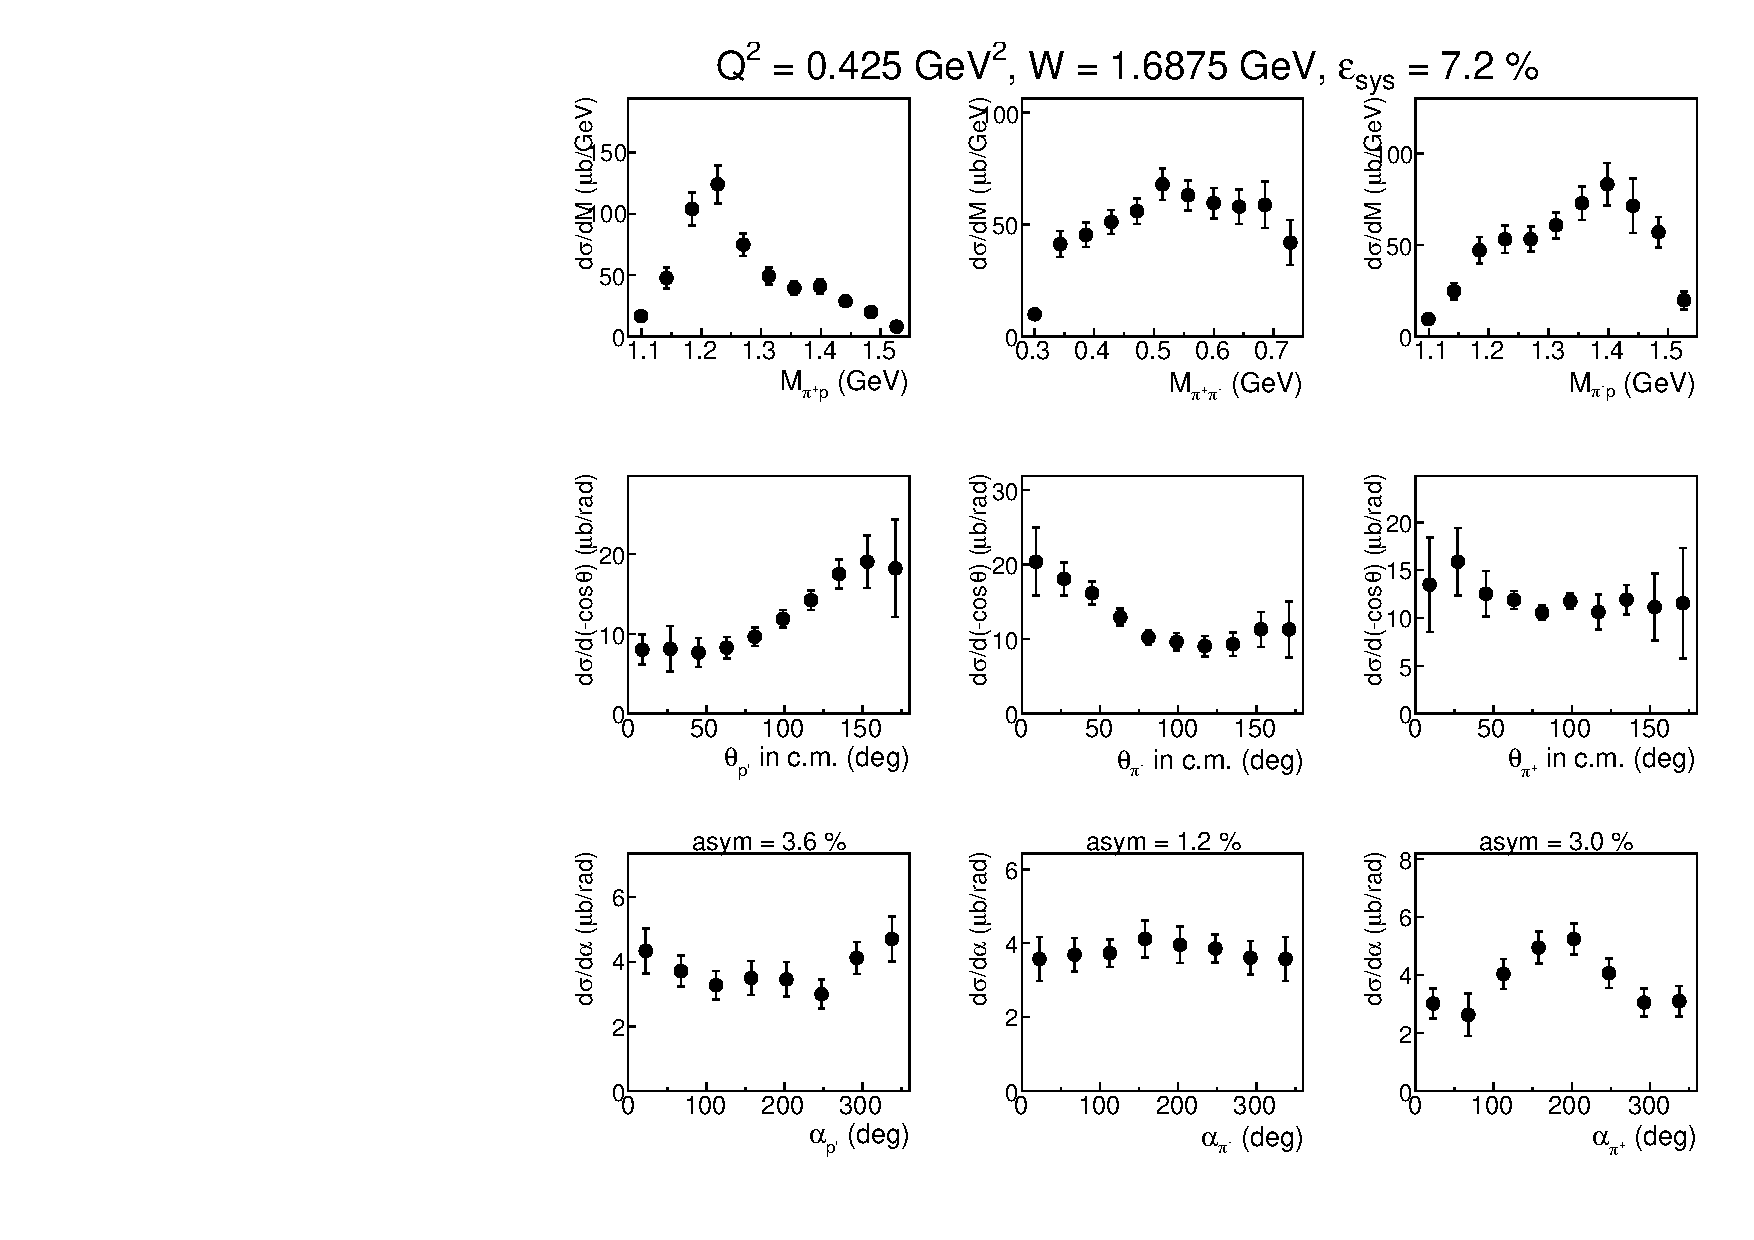
\includegraphics[width=0.45\textwidth]{pictures/appendix/1diff_distr/Q2_425/w_16875.pdf}}
\caption{\small } \label{fig:appx_1}
\end{center}
\end{figure}

\clearpage
\begin{figure}[htp]
\begin{center}
\frame{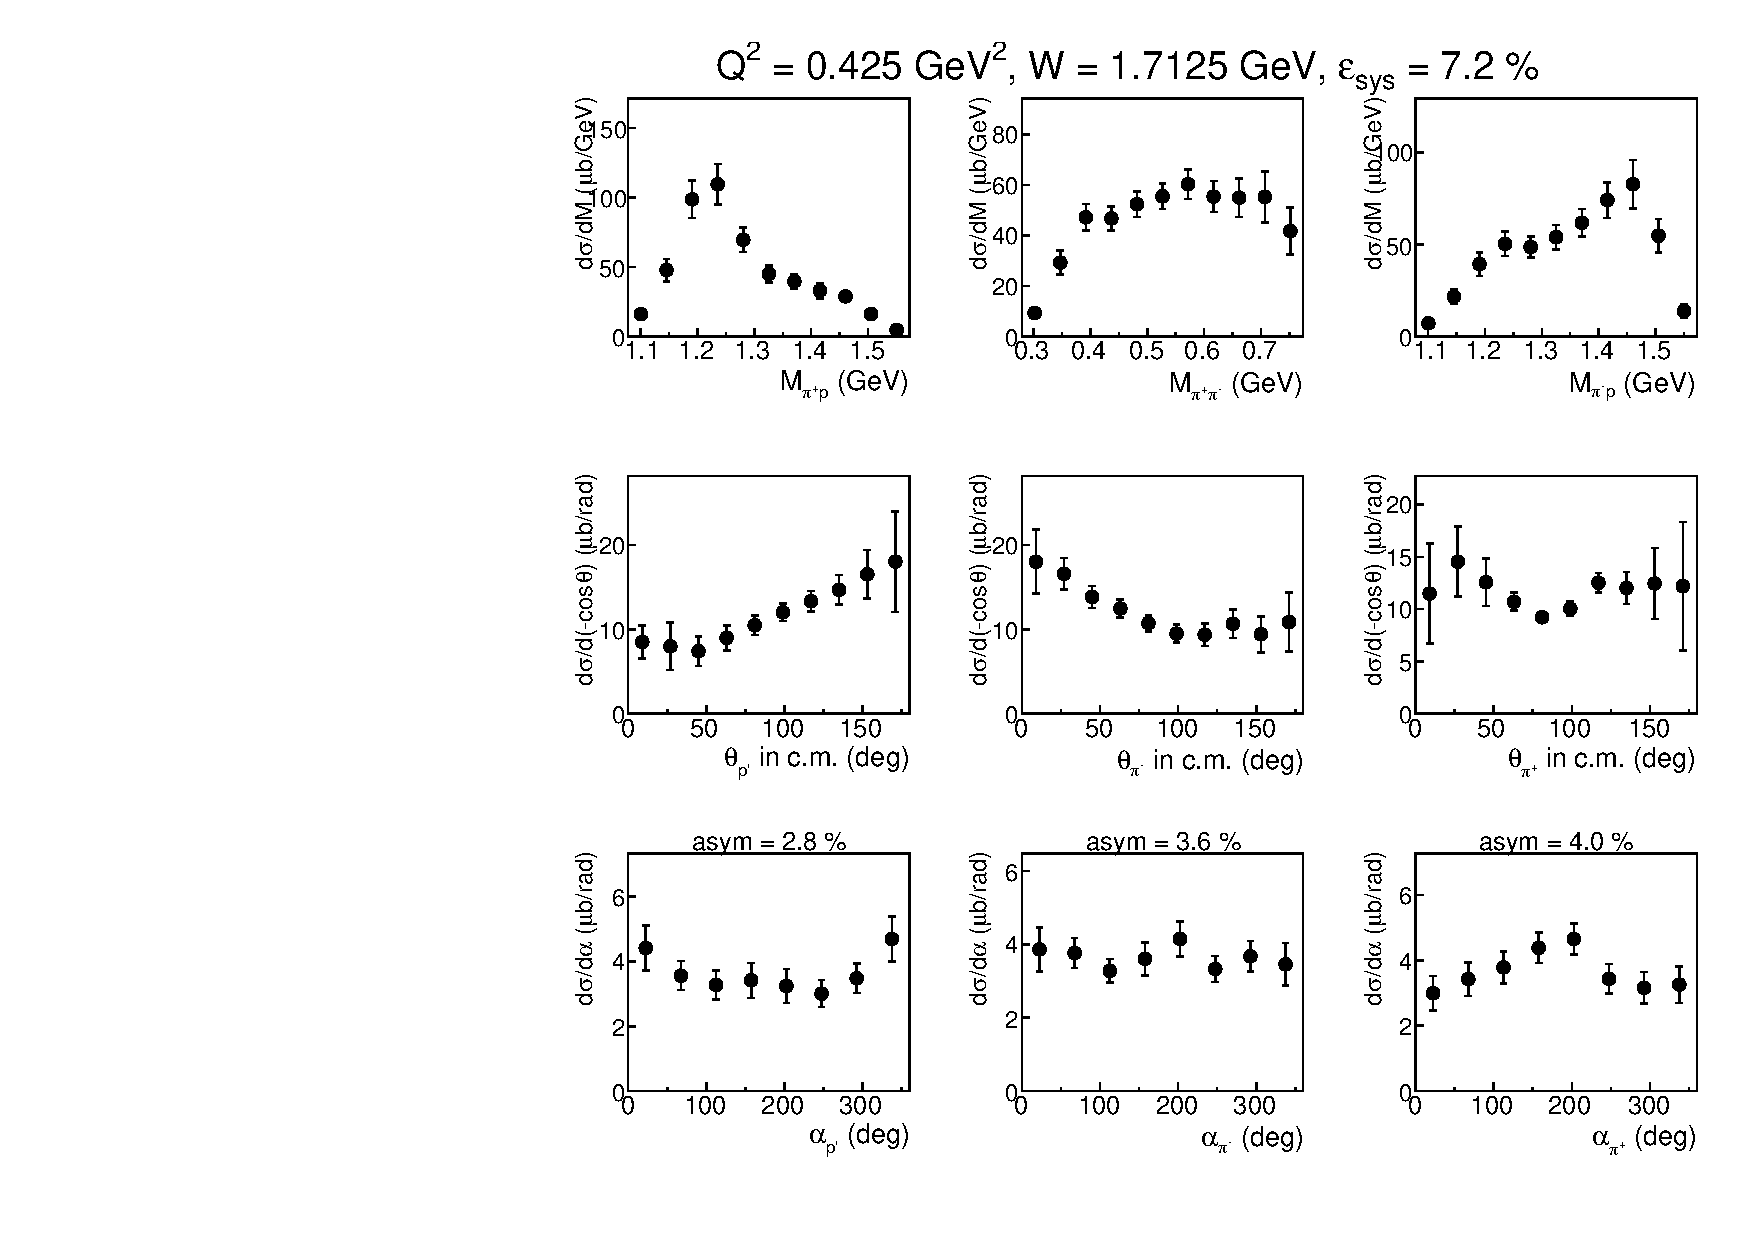
\includegraphics[width=0.45\textwidth]{pictures/appendix/1diff_distr/Q2_425/w_17125.pdf}}
\frame{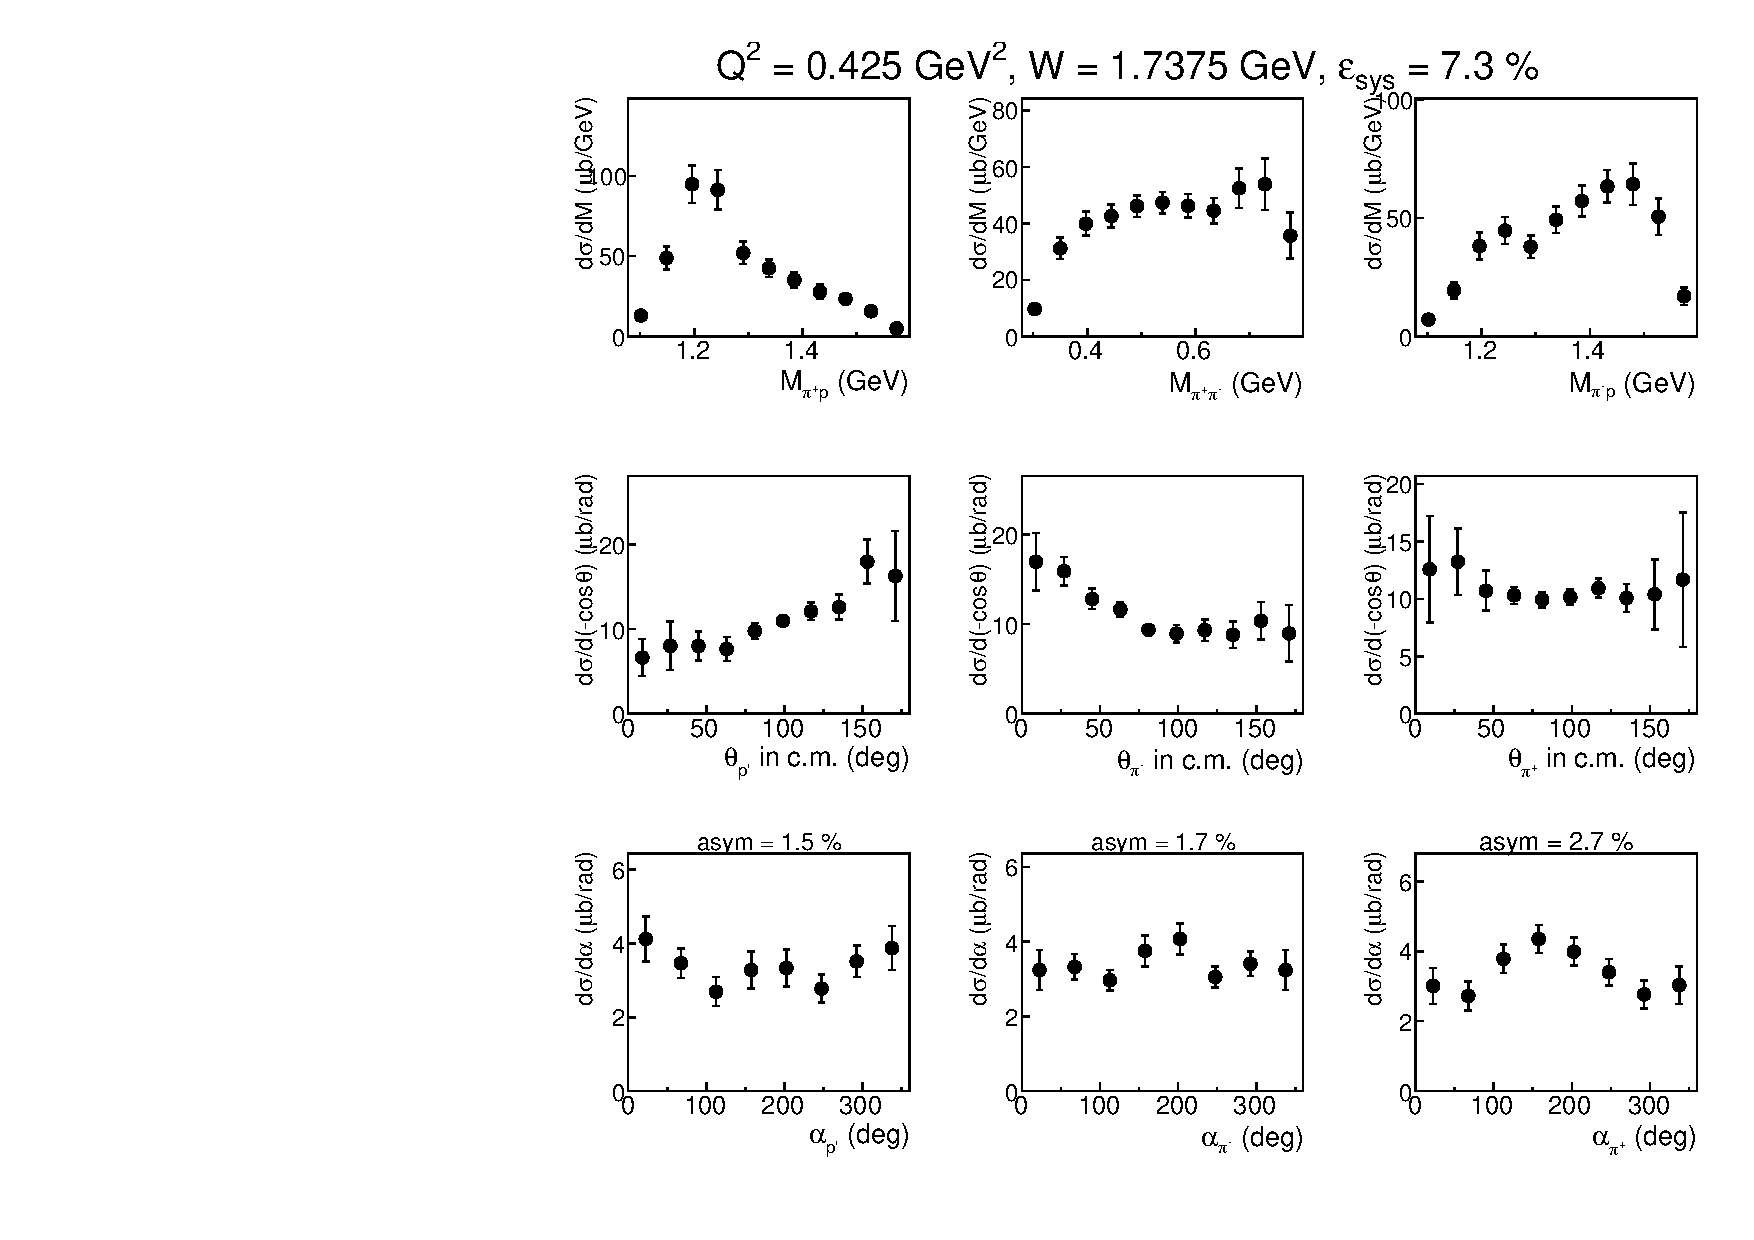
\includegraphics[width=0.45\textwidth]{pictures/appendix/1diff_distr/Q2_425/w_17375.pdf}}
\frame{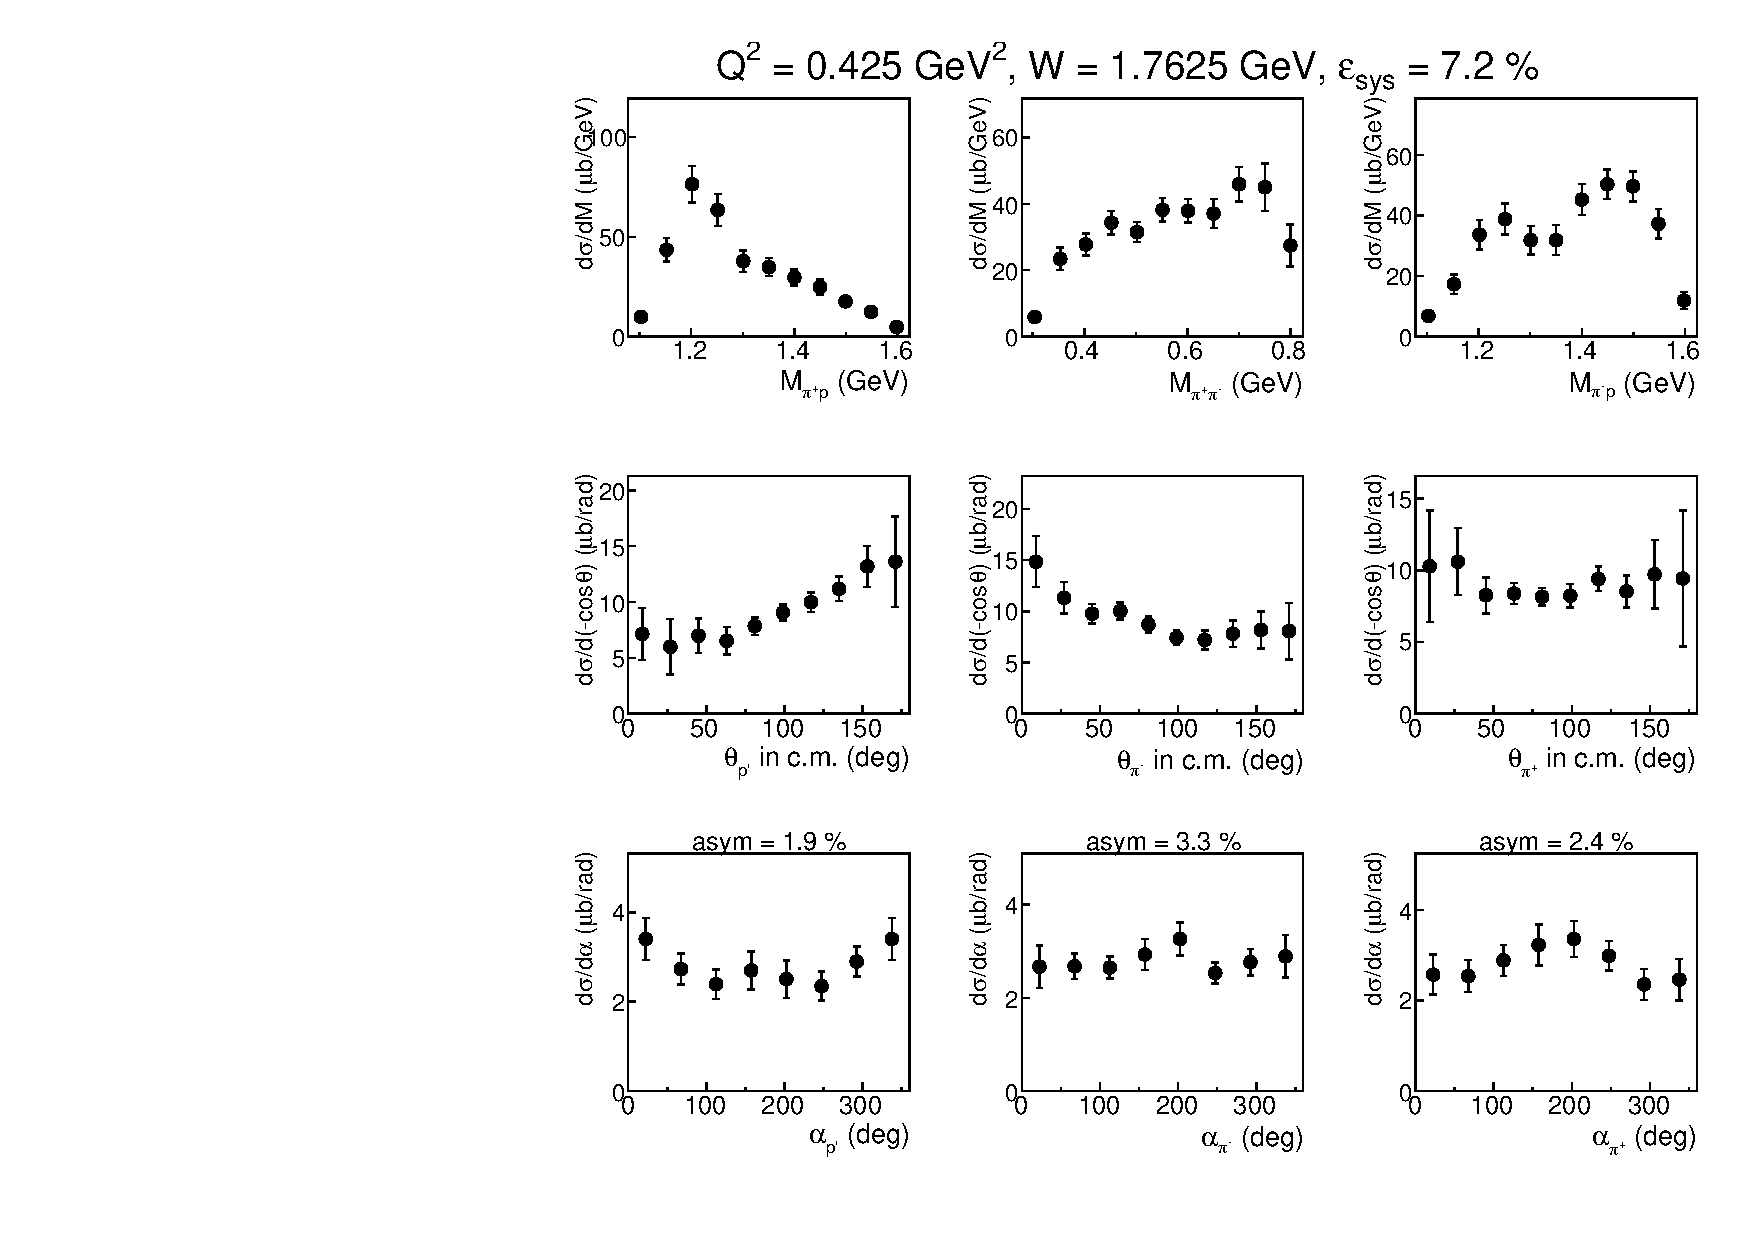
\includegraphics[width=0.45\textwidth]{pictures/appendix/1diff_distr/Q2_425/w_17625.pdf}}
\frame{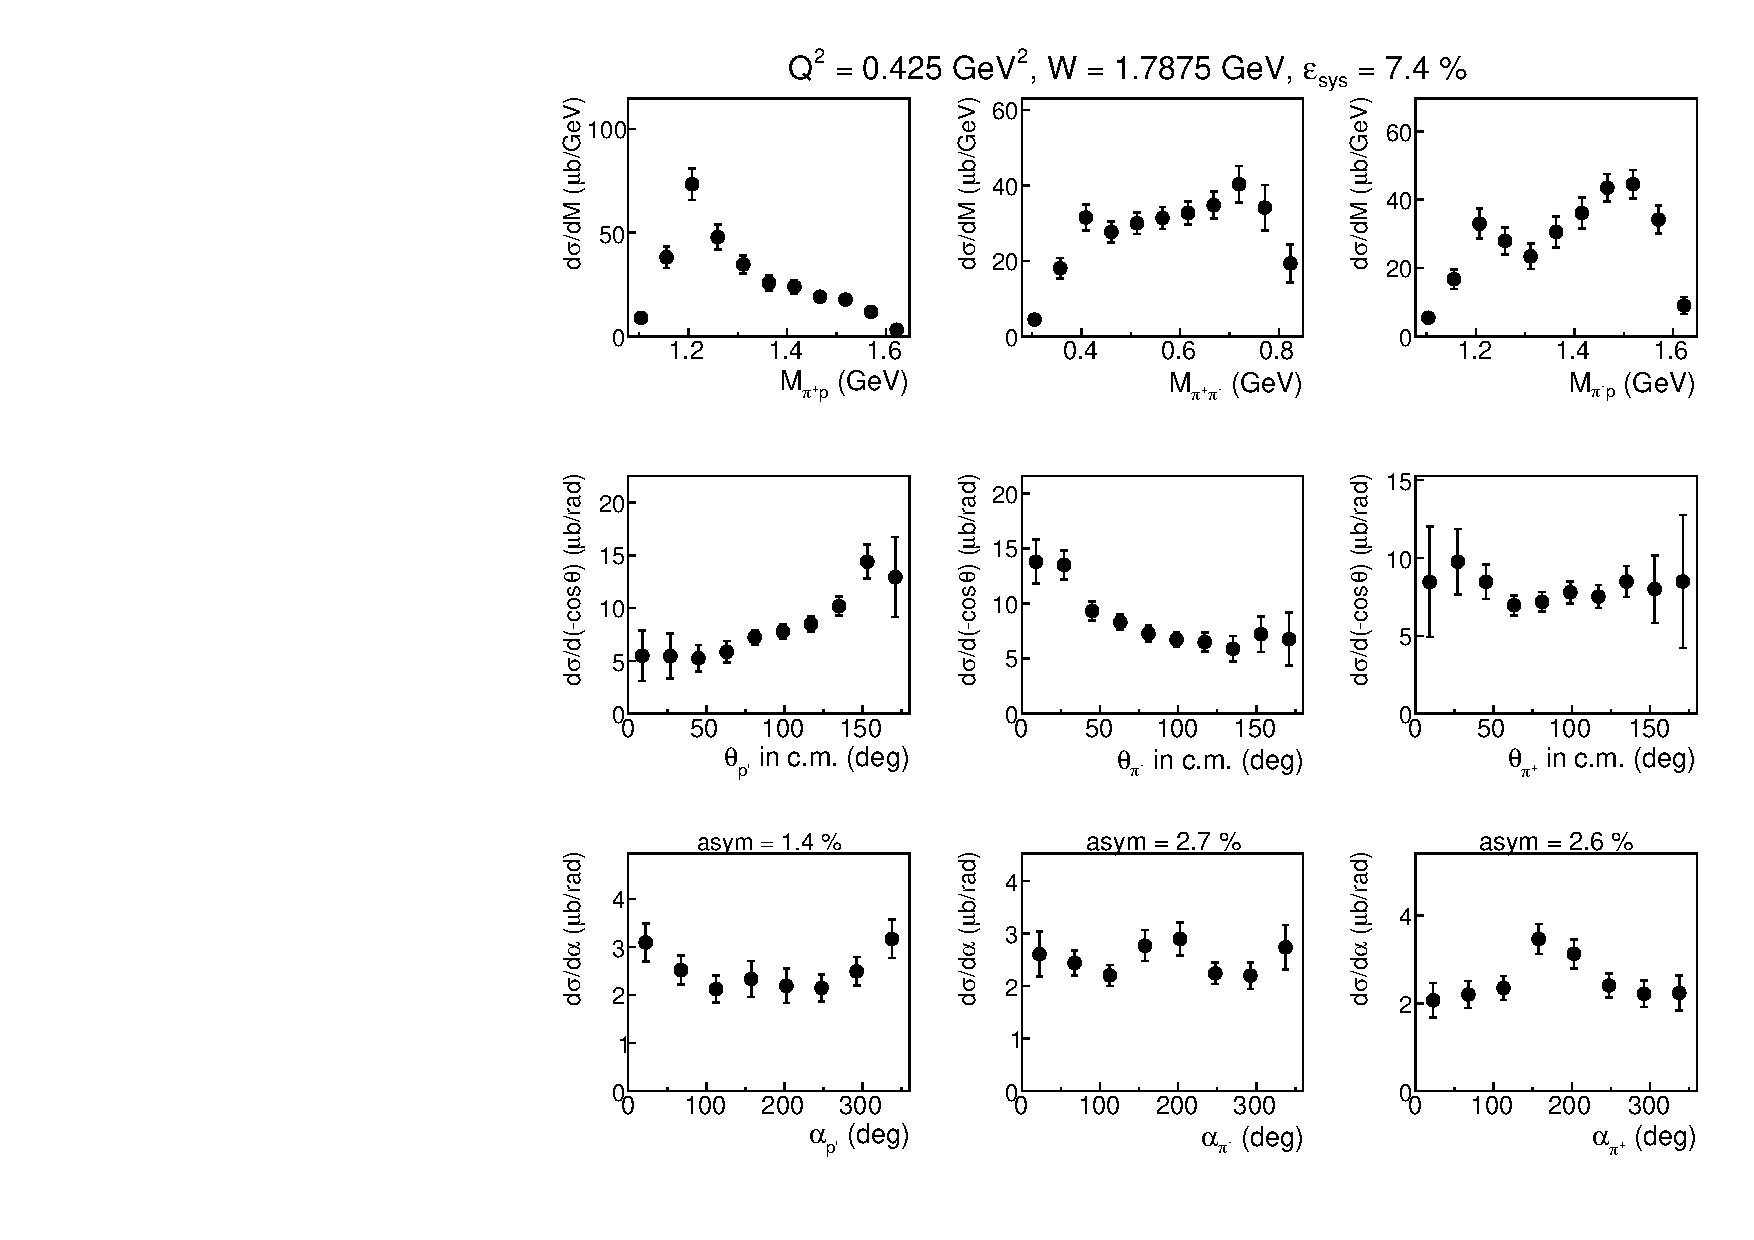
\includegraphics[width=0.45\textwidth]{pictures/appendix/1diff_distr/Q2_425/w_17875.pdf}}
\caption{\small } \label{fig:appx_2}
\end{center}
\end{figure}

\clearpage
\begin{figure}[htp]
\begin{center}
\frame{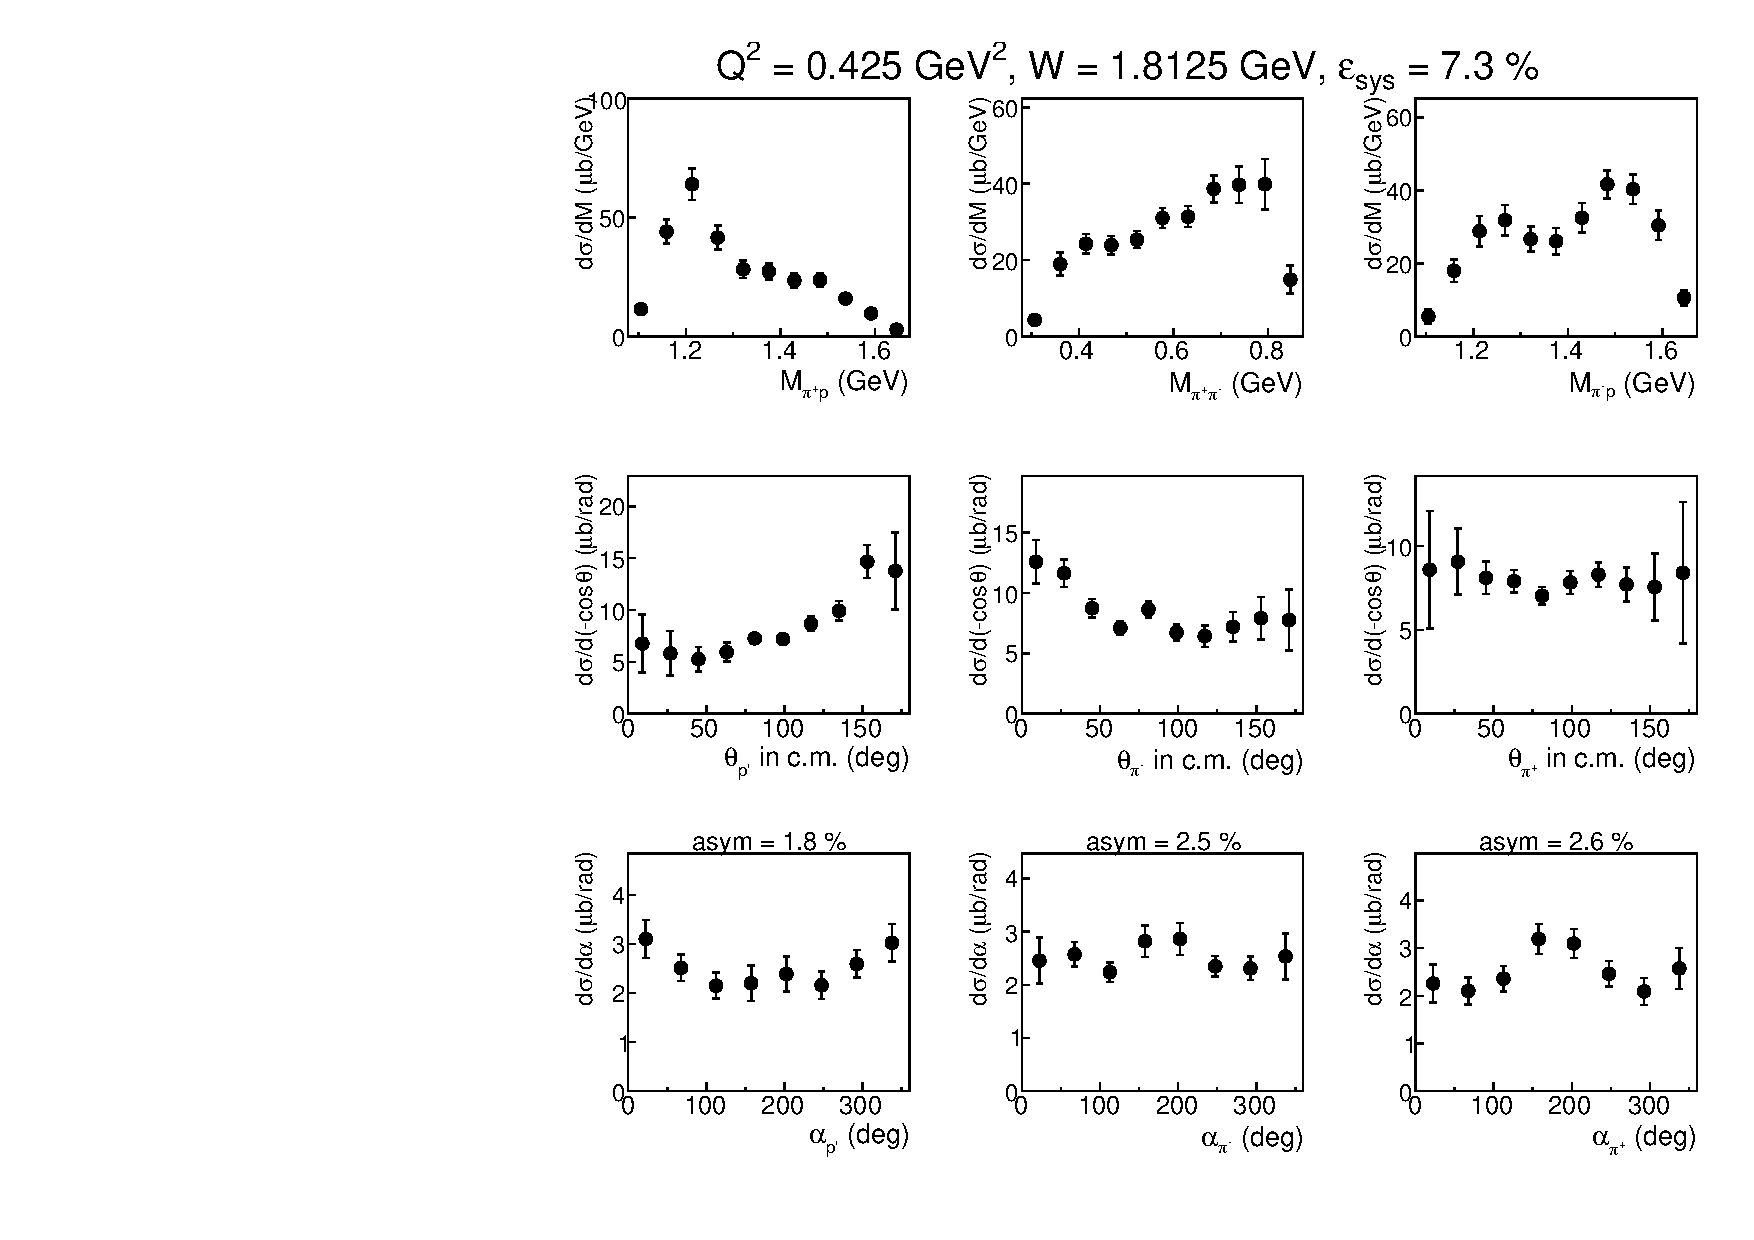
\includegraphics[width=0.45\textwidth]{pictures/appendix/1diff_distr/Q2_425/w_18125.pdf}}
\frame{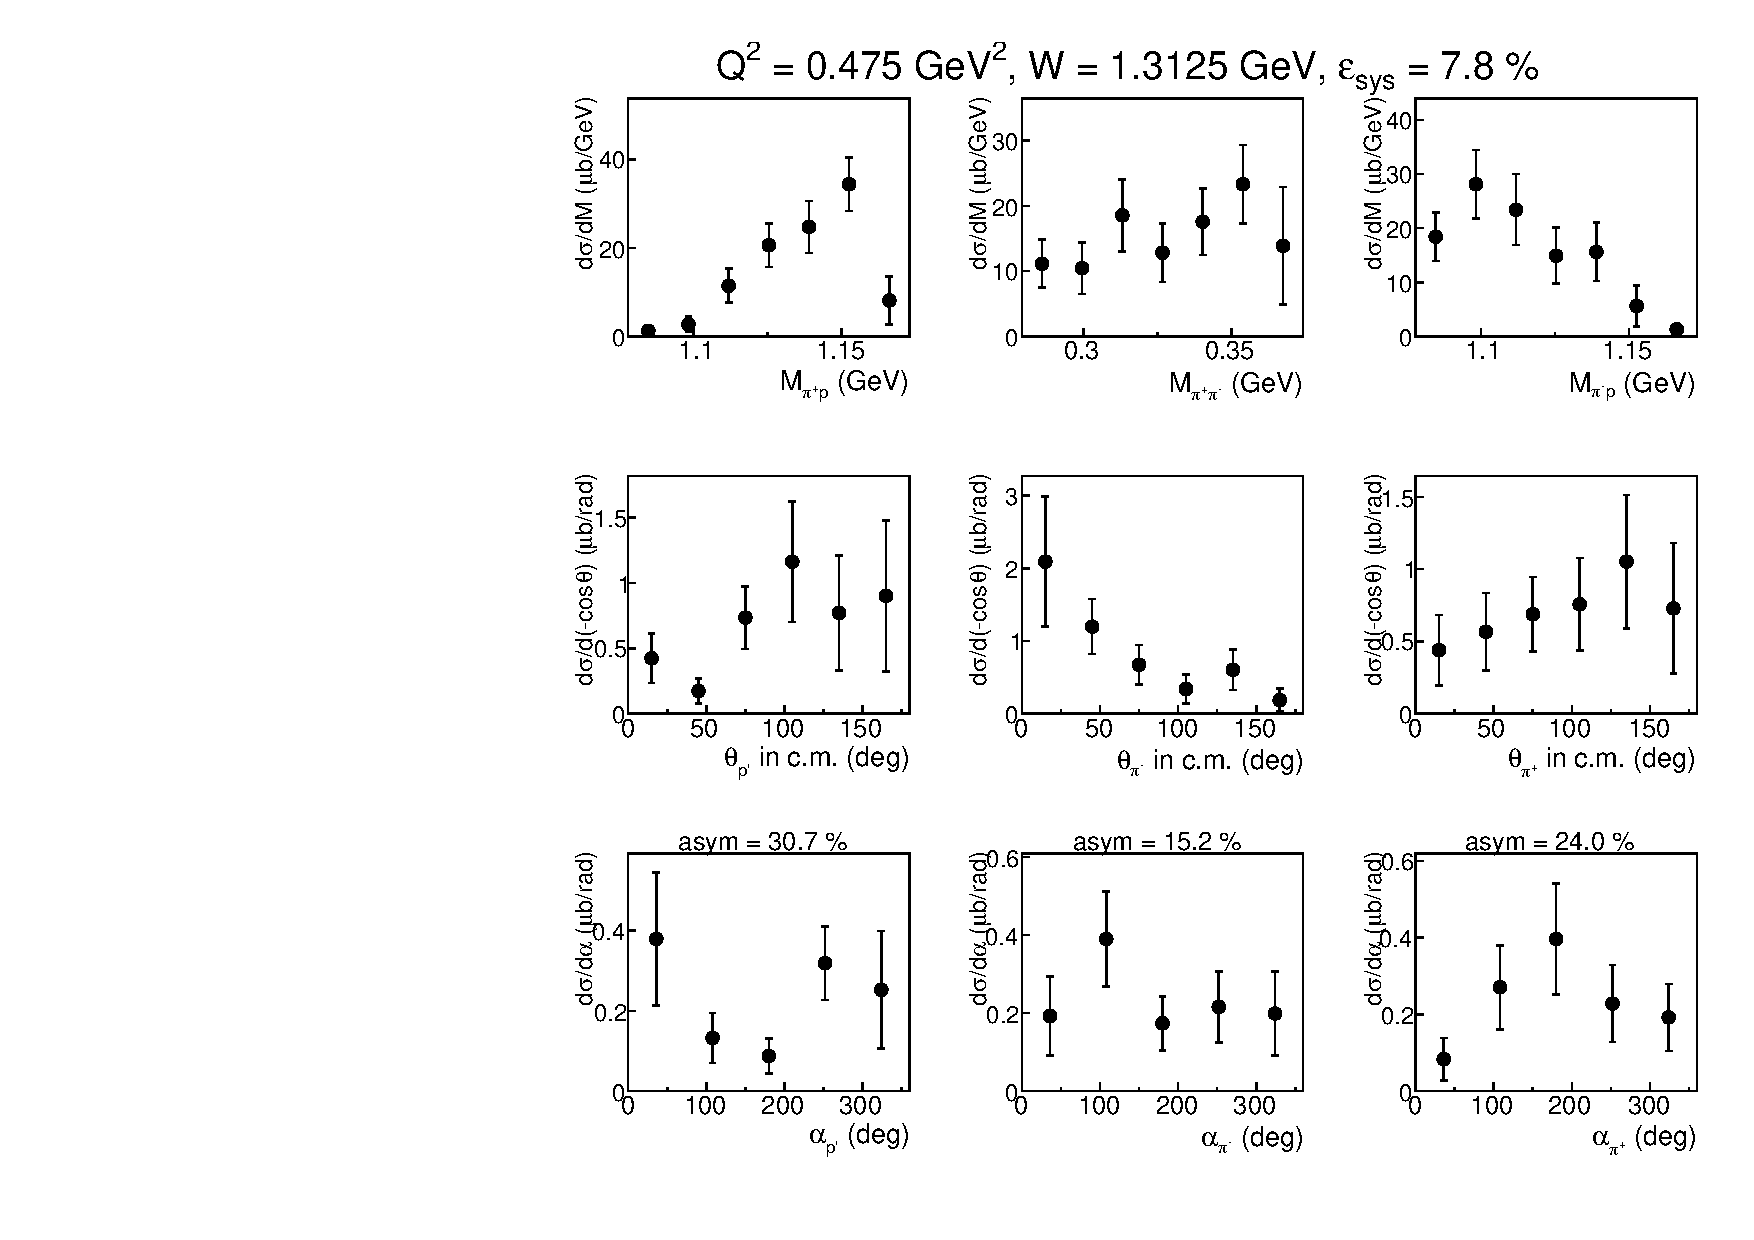
\includegraphics[width=0.45\textwidth]{pictures/appendix/1diff_distr/Q2_475/w_13125.pdf}}
\frame{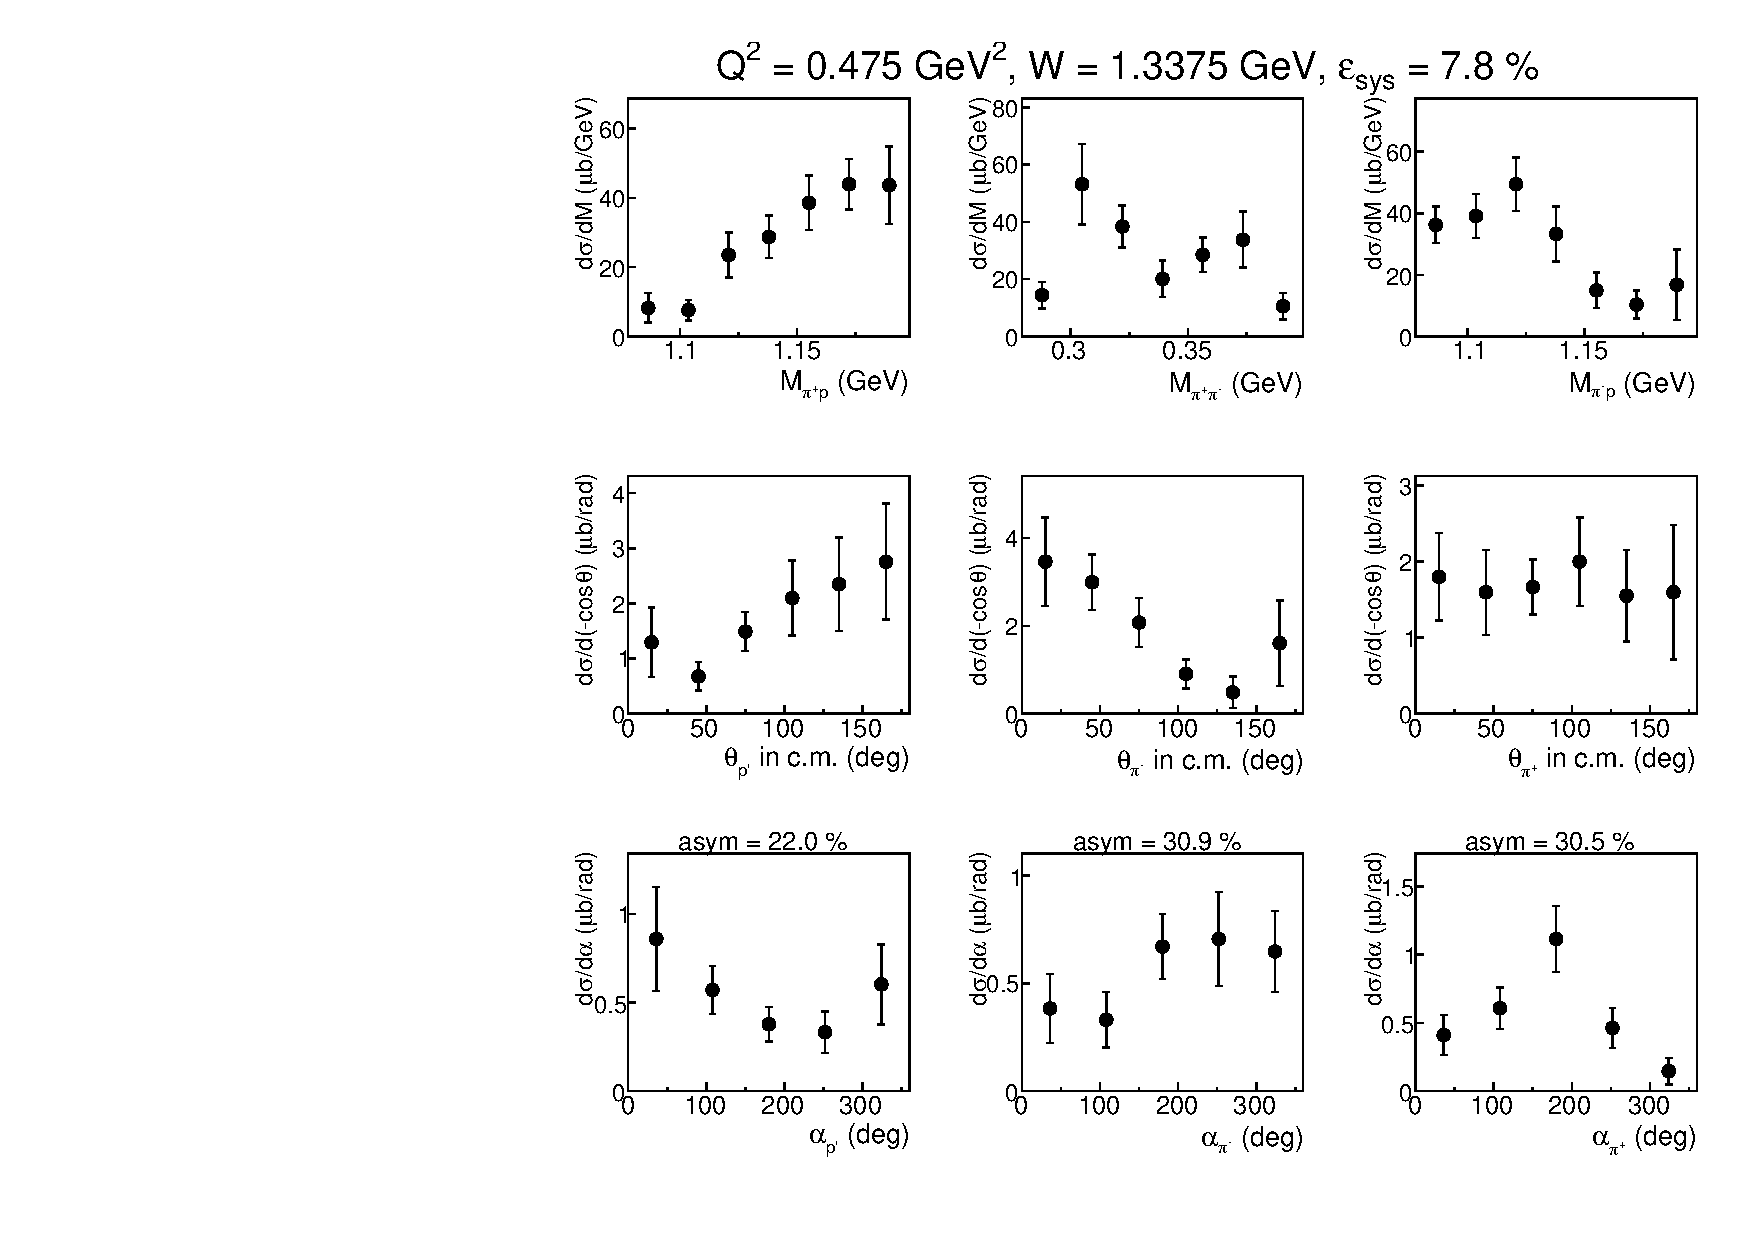
\includegraphics[width=0.45\textwidth]{pictures/appendix/1diff_distr/Q2_475/w_13375.pdf}}
\frame{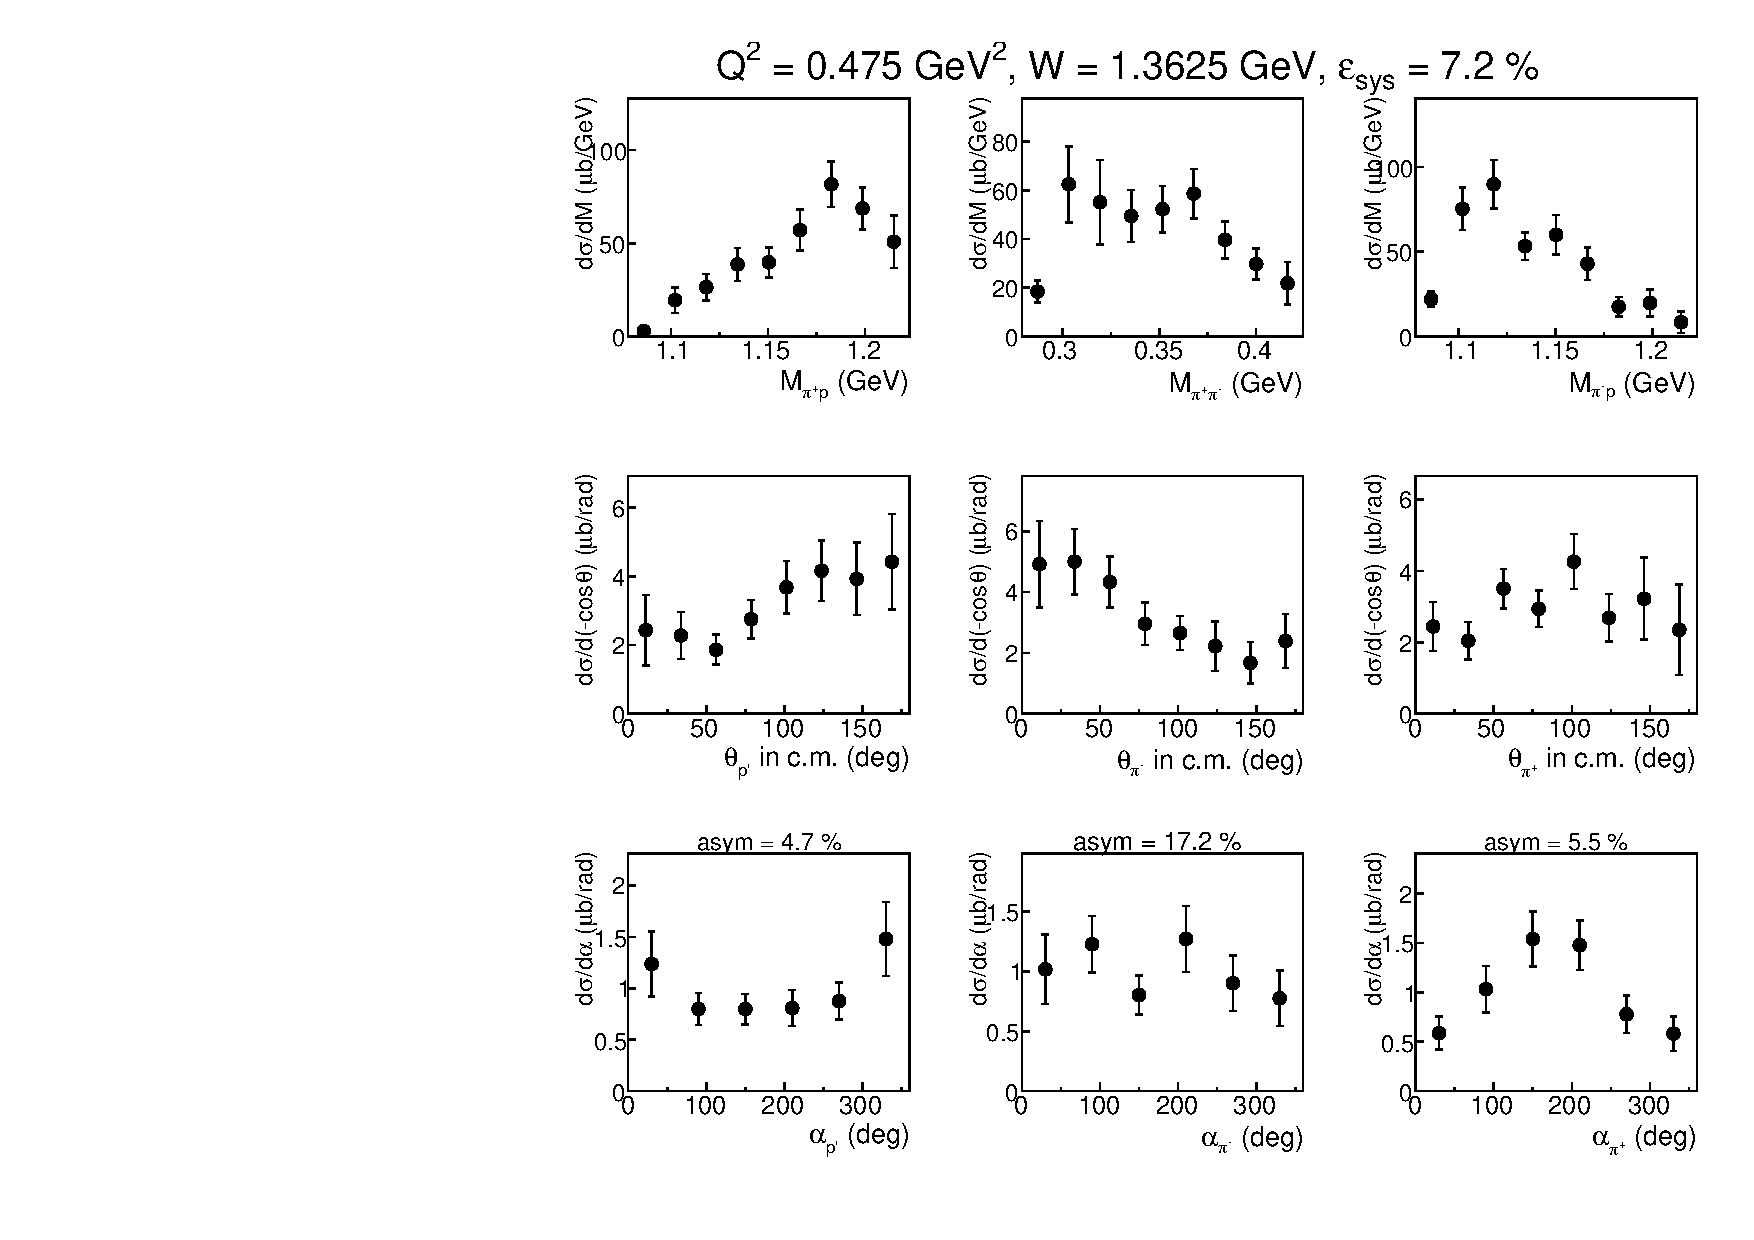
\includegraphics[width=0.45\textwidth]{pictures/appendix/1diff_distr/Q2_475/w_13625.pdf}}
\caption{\small } \label{fig:appx_3}
\end{center}
\end{figure}

\clearpage
\begin{figure}[htp]
\begin{center}
\frame{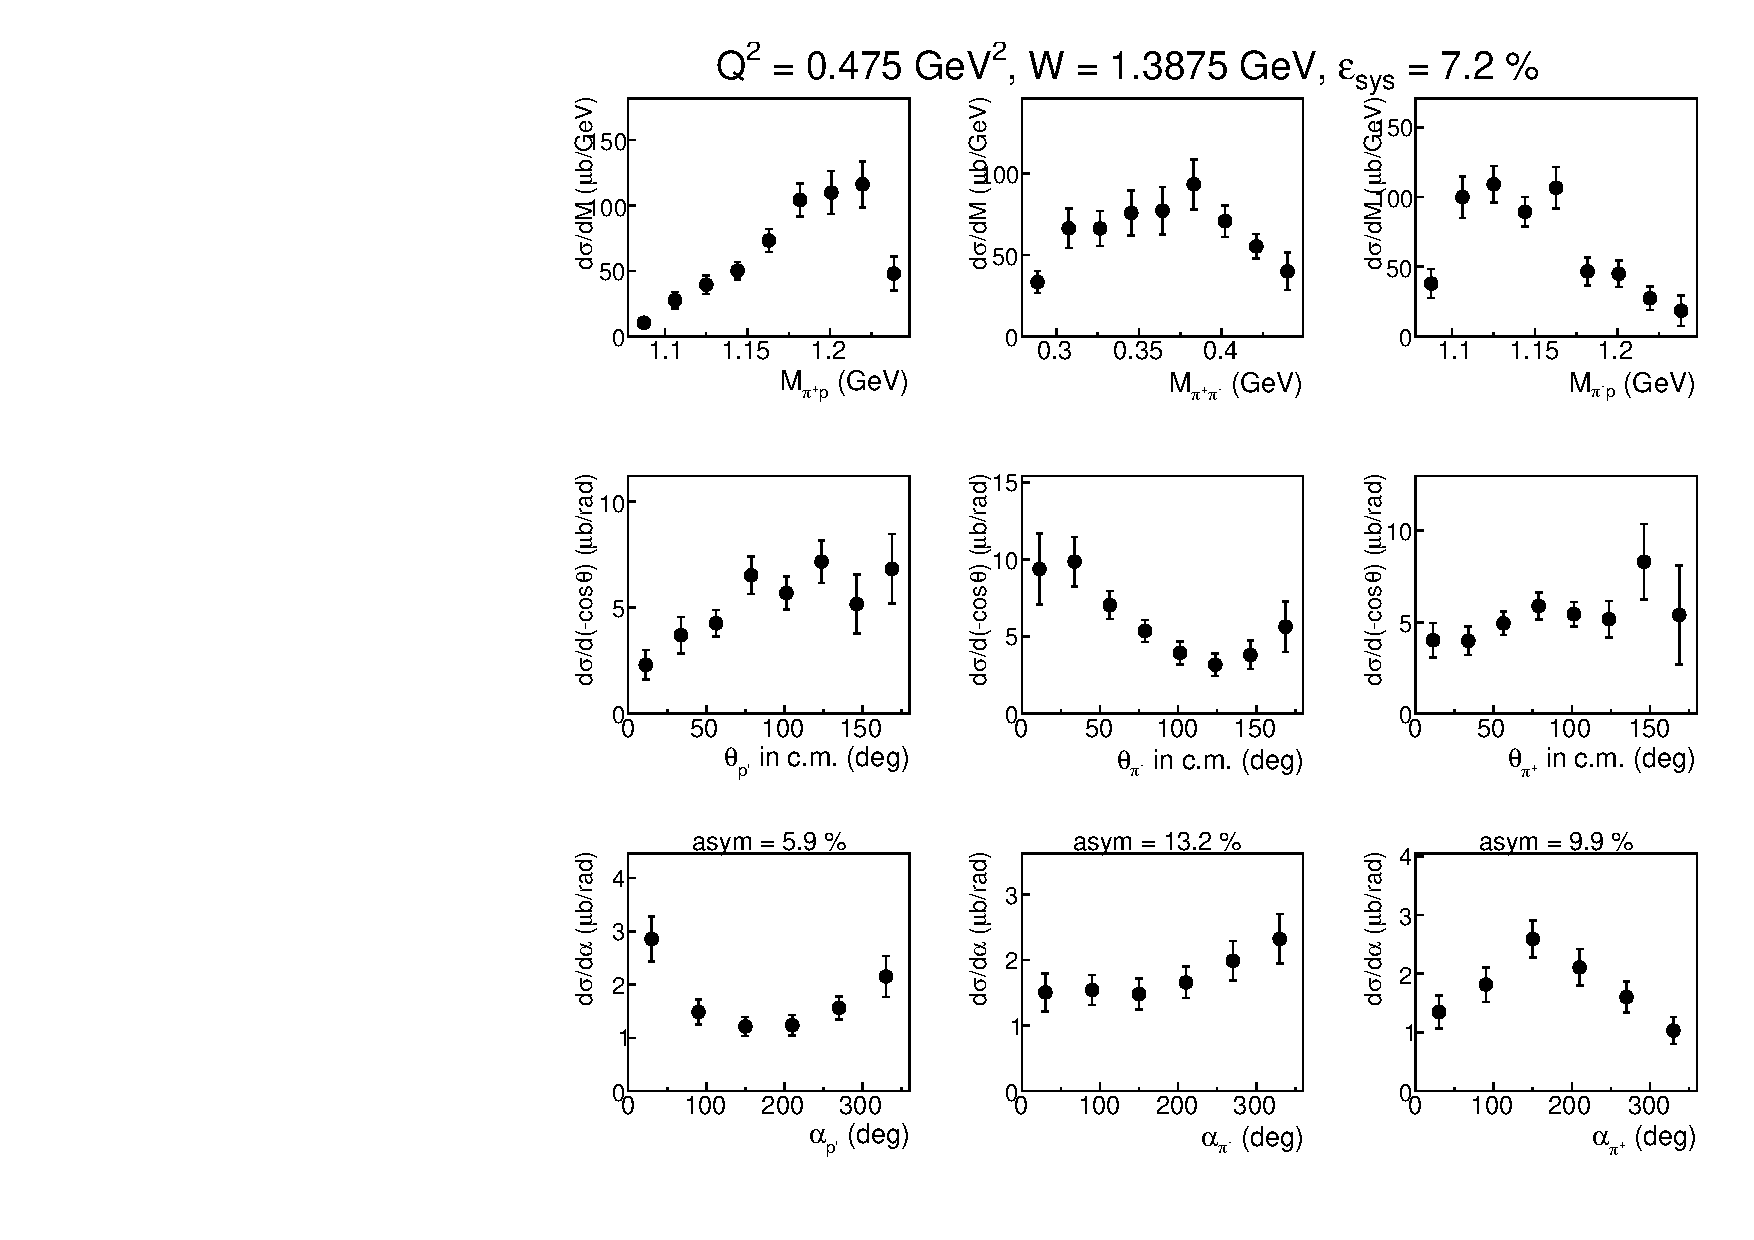
\includegraphics[width=0.45\textwidth]{pictures/appendix/1diff_distr/Q2_475/w_13875.pdf}}
\frame{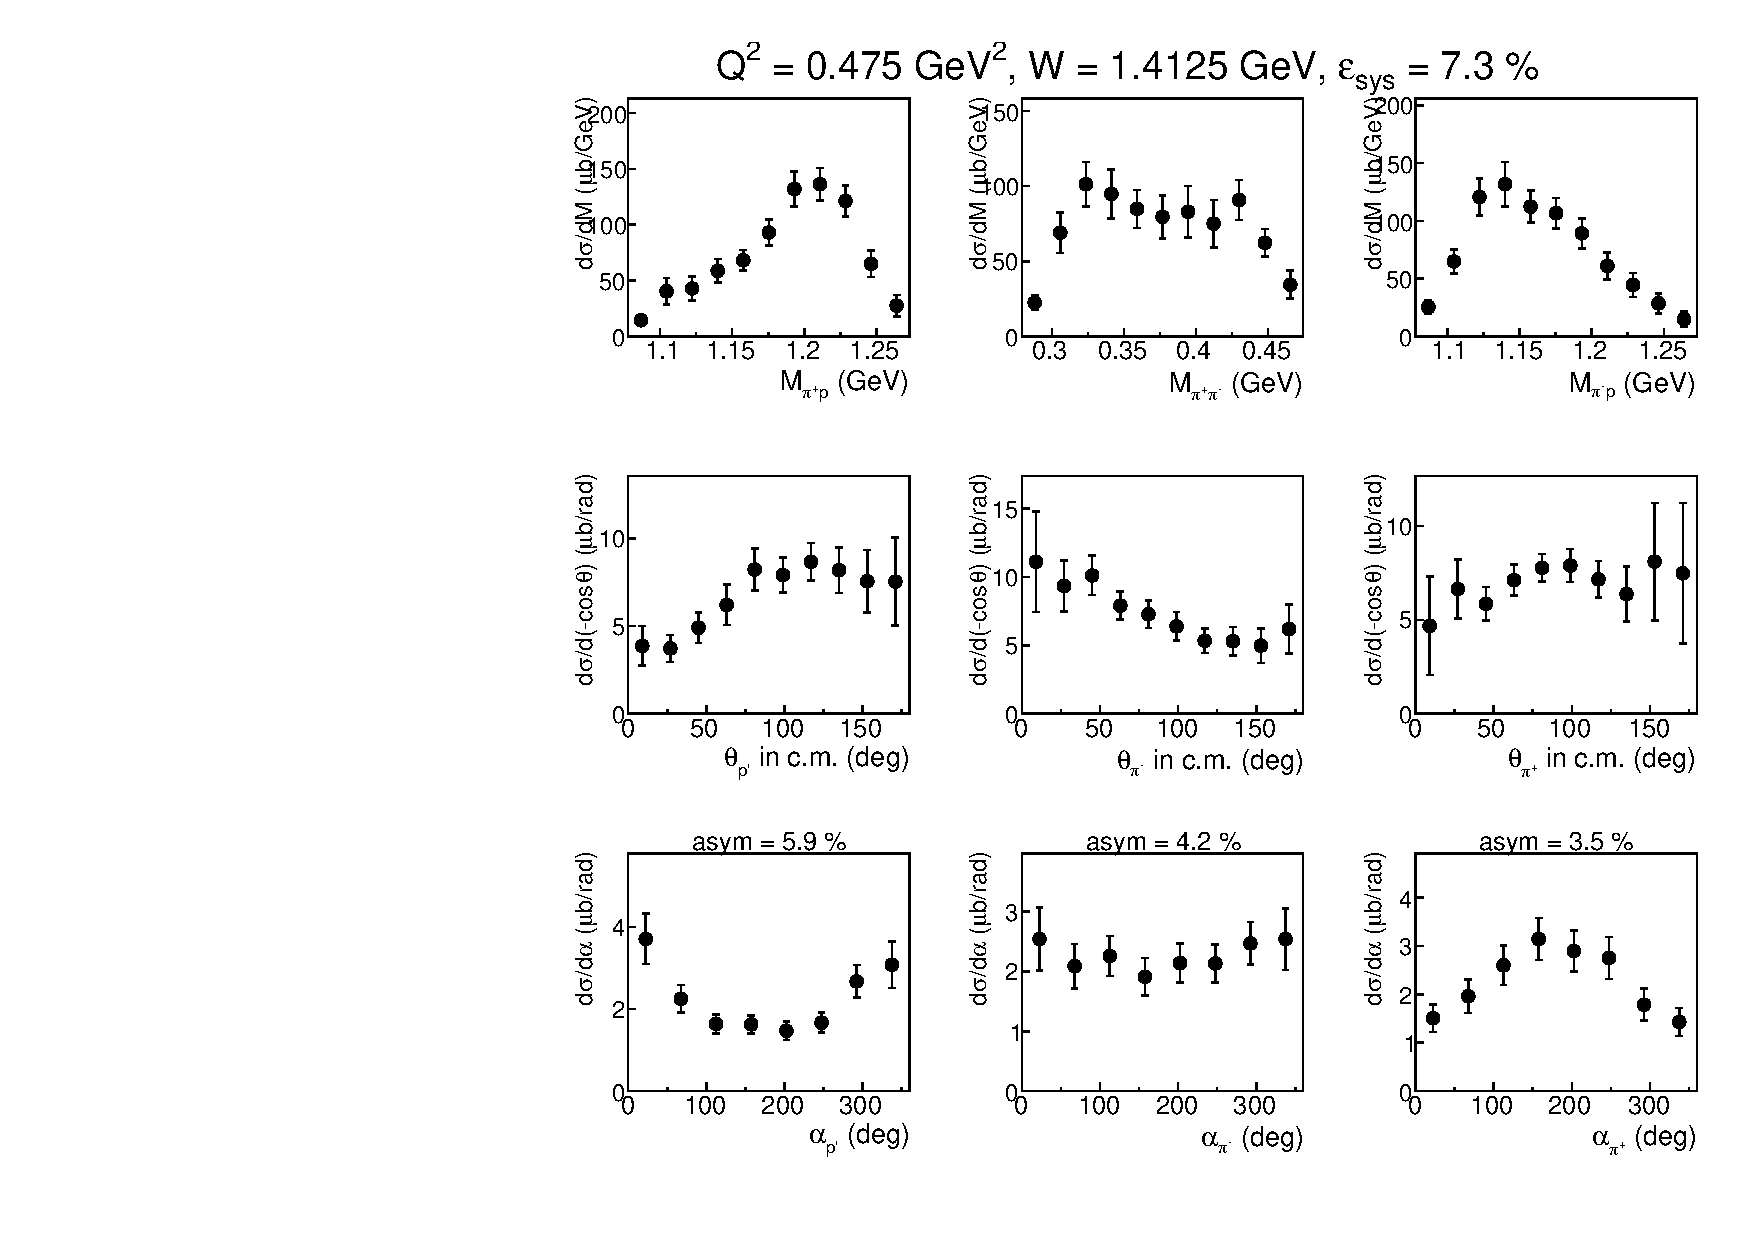
\includegraphics[width=0.45\textwidth]{pictures/appendix/1diff_distr/Q2_475/w_14125.pdf}}
\frame{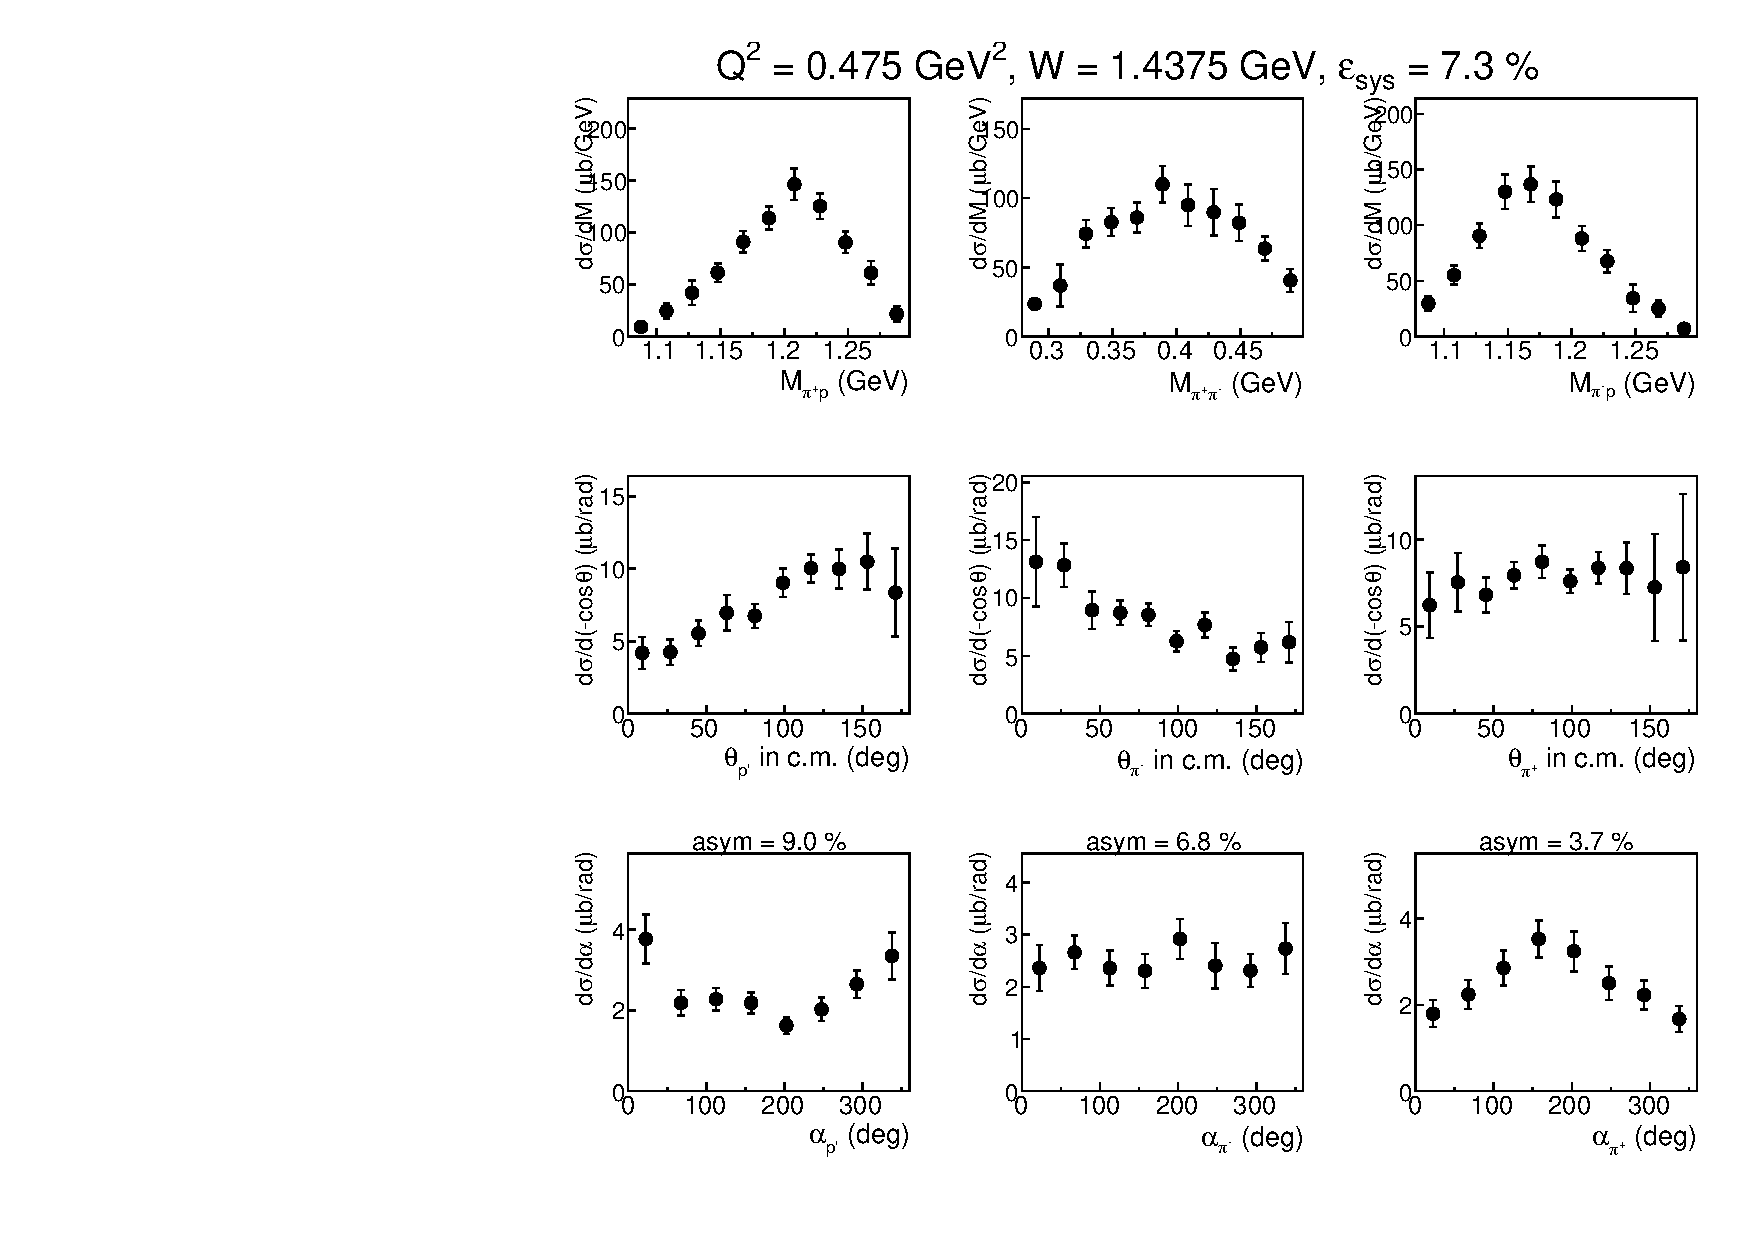
\includegraphics[width=0.45\textwidth]{pictures/appendix/1diff_distr/Q2_475/w_14375.pdf}}
\frame{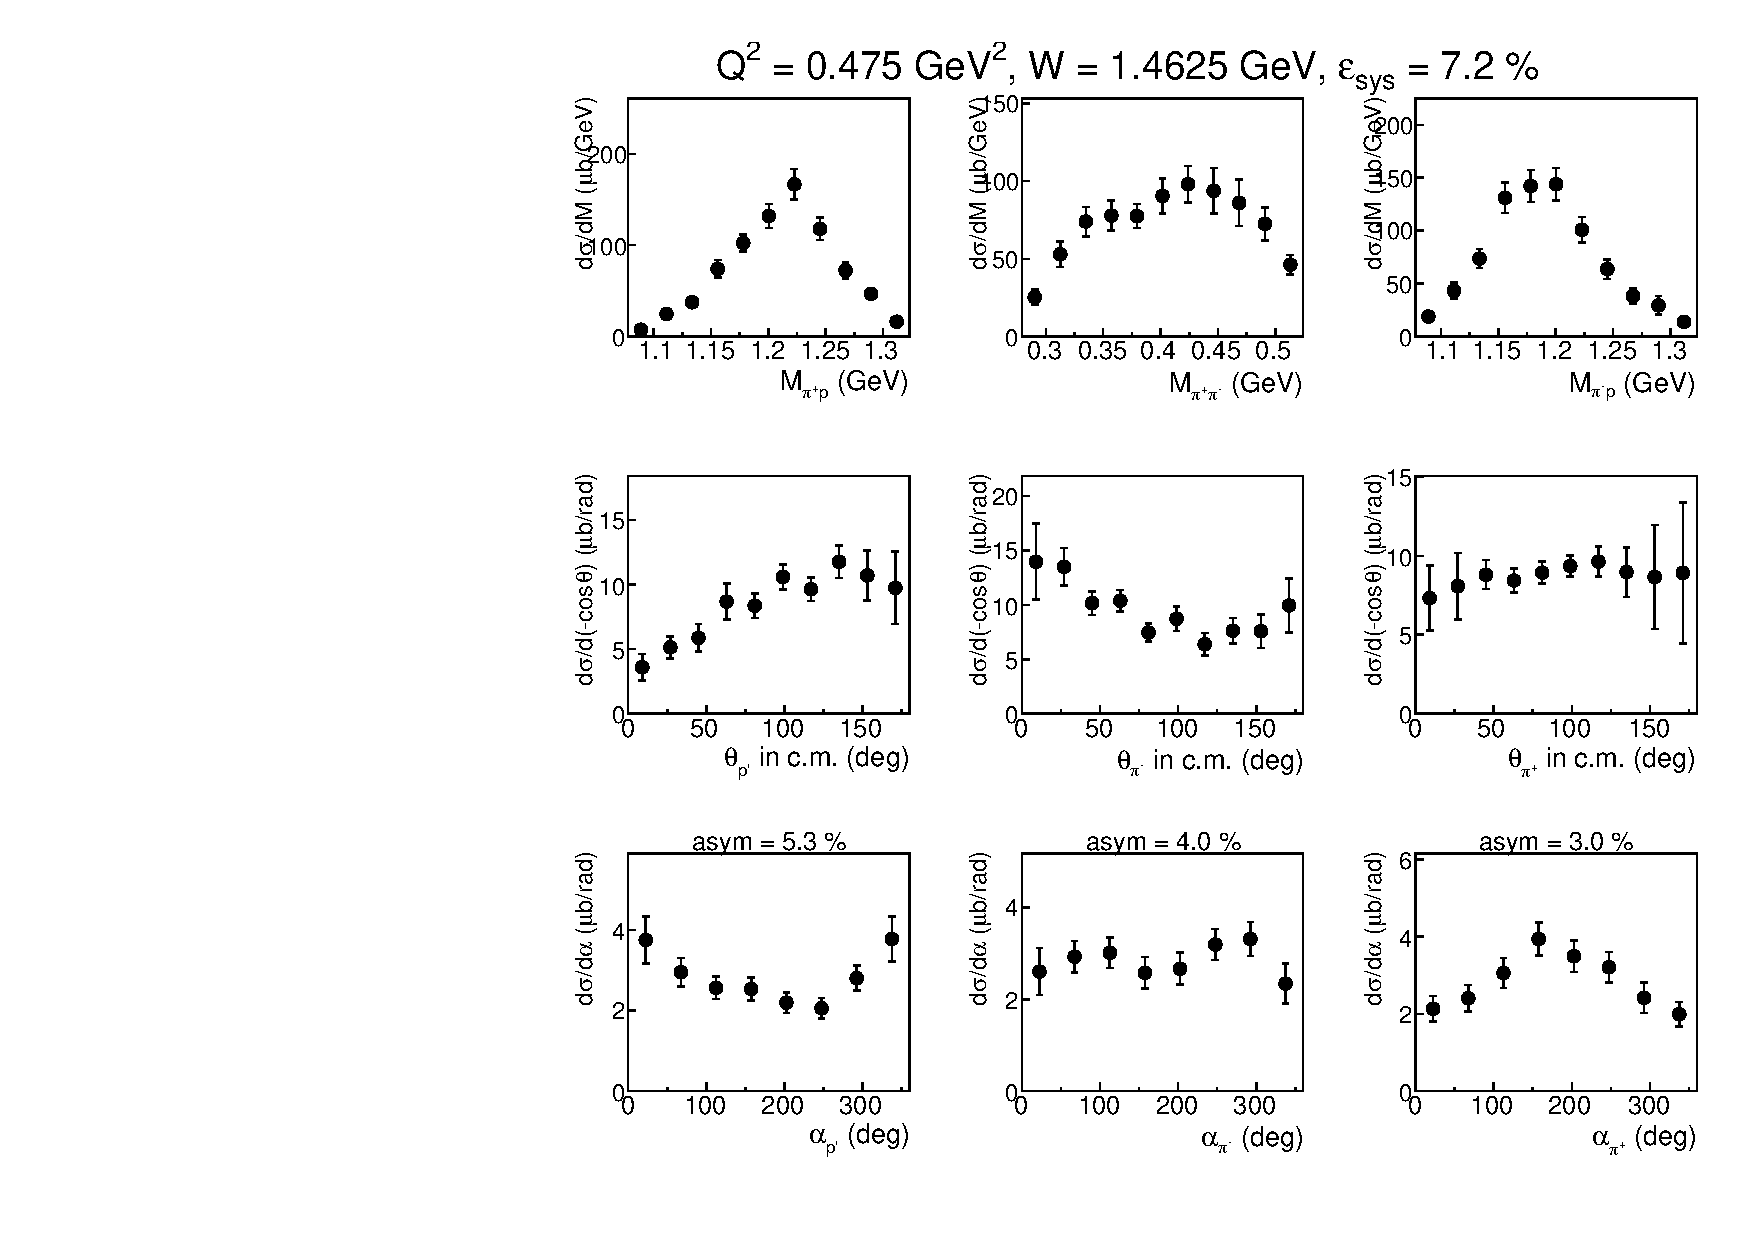
\includegraphics[width=0.45\textwidth]{pictures/appendix/1diff_distr/Q2_475/w_14625.pdf}}
\caption{\small } \label{fig:appx_4}
\end{center}
\end{figure}

\clearpage
\begin{figure}[htp]
\begin{center}
\frame{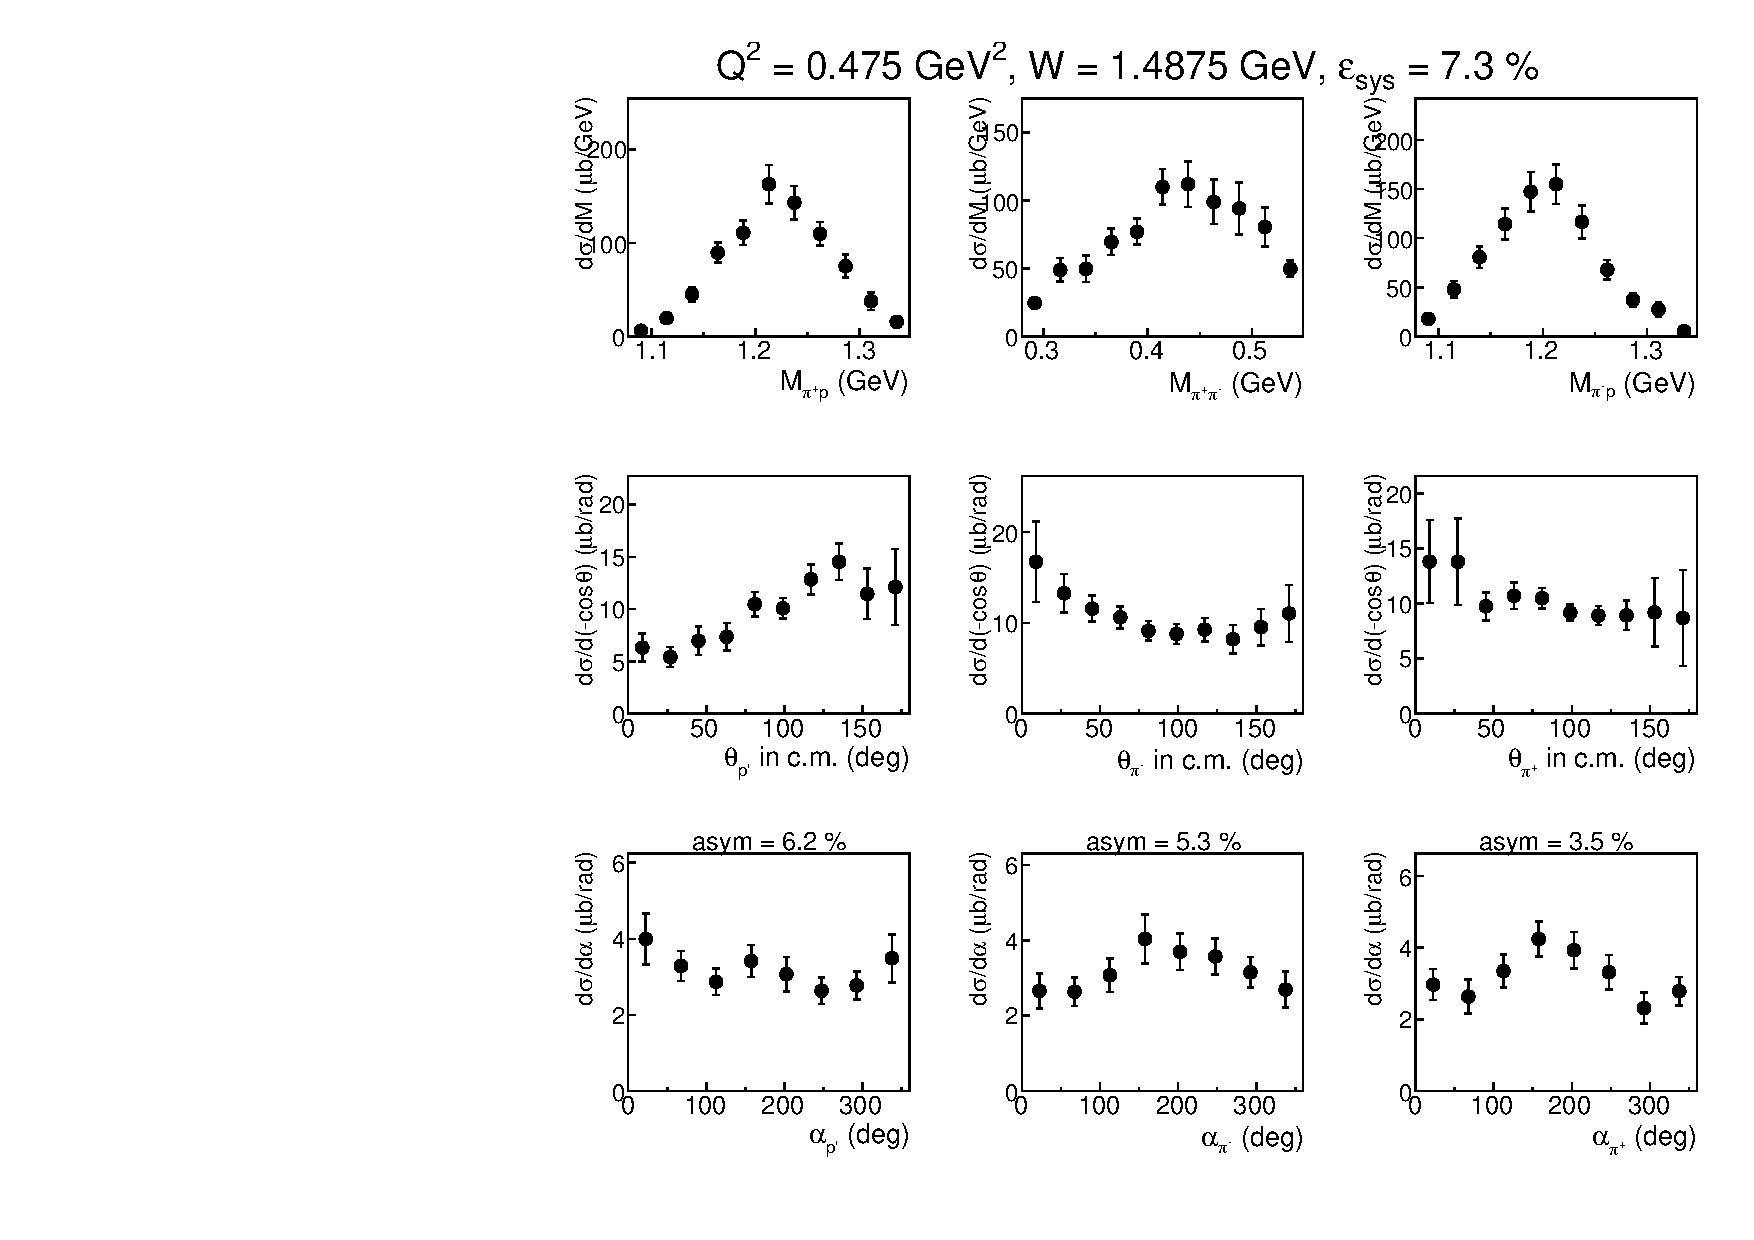
\includegraphics[width=0.45\textwidth]{pictures/appendix/1diff_distr/Q2_475/w_14875.pdf}}
\frame{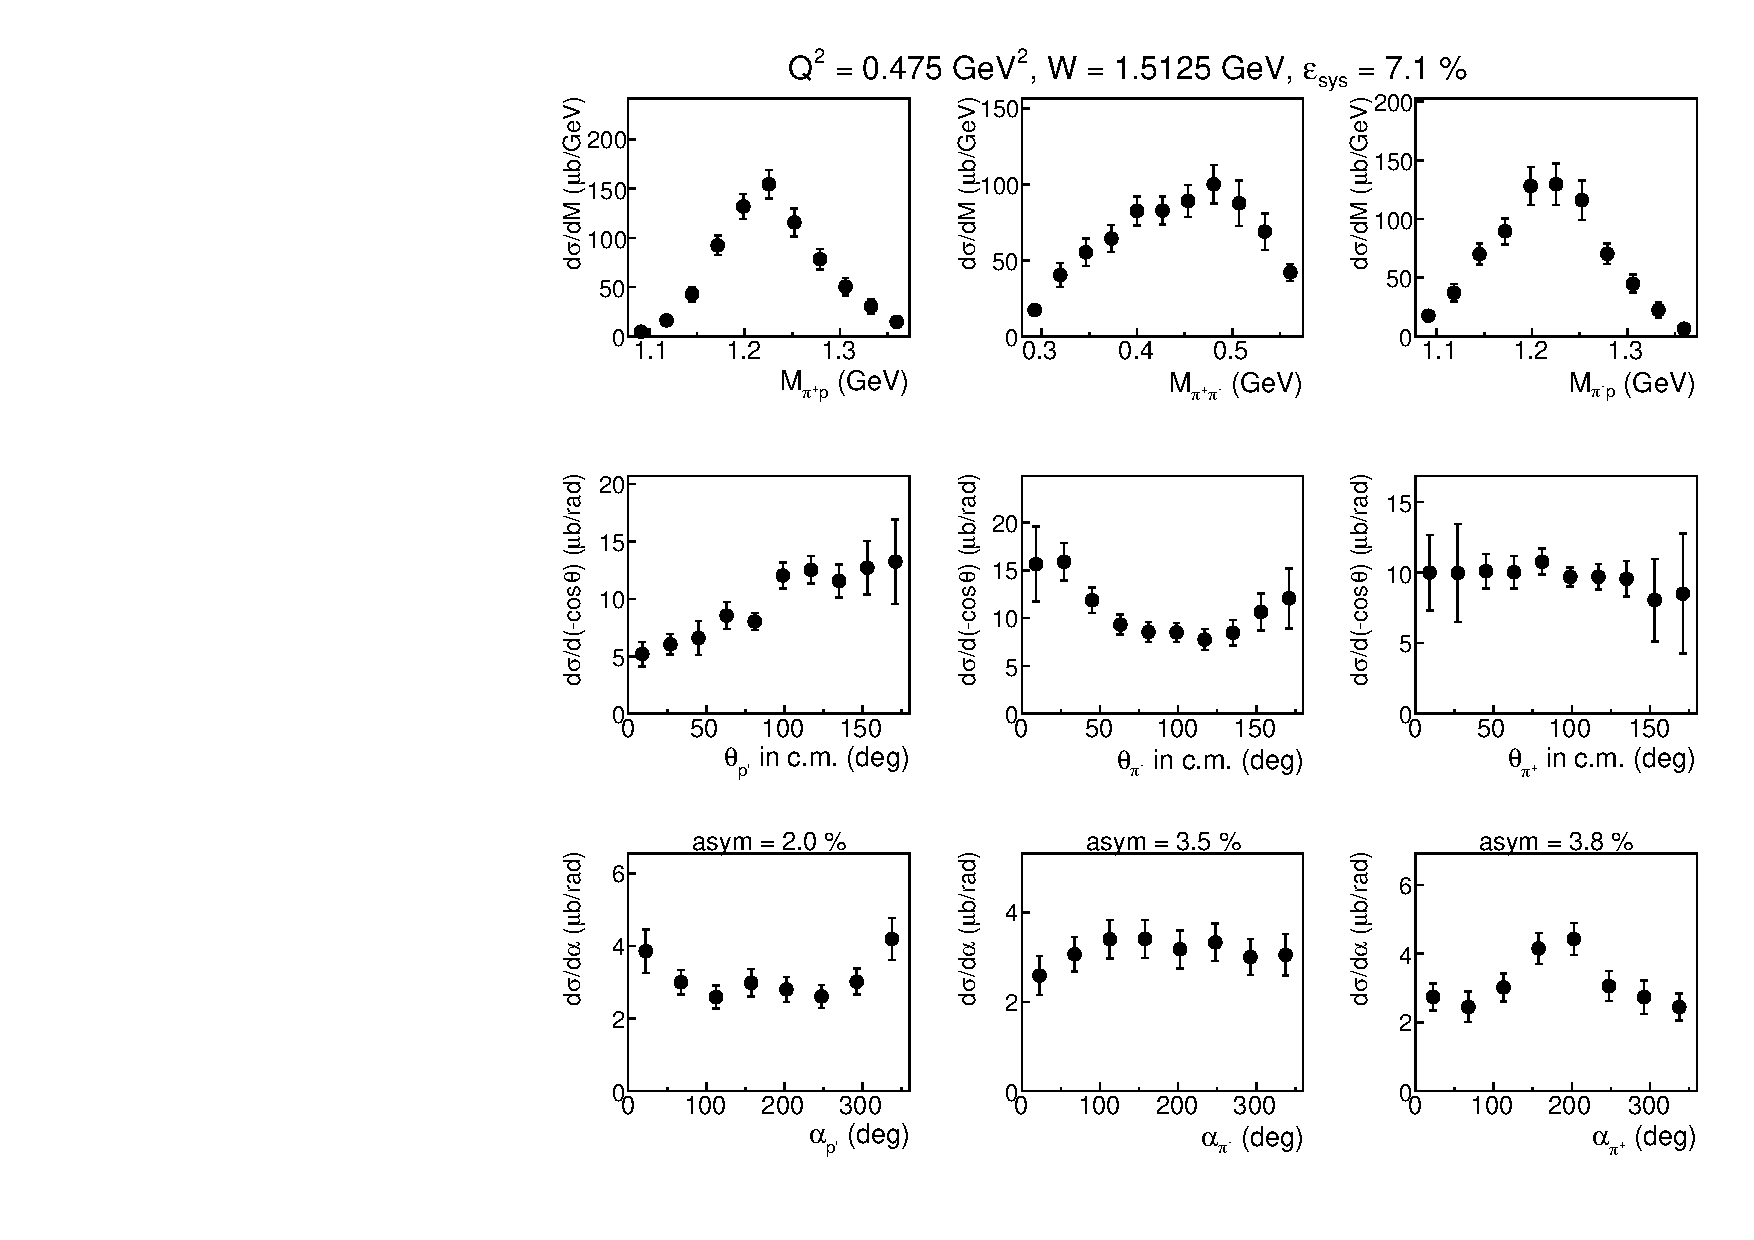
\includegraphics[width=0.45\textwidth]{pictures/appendix/1diff_distr/Q2_475/w_15125.pdf}}
\frame{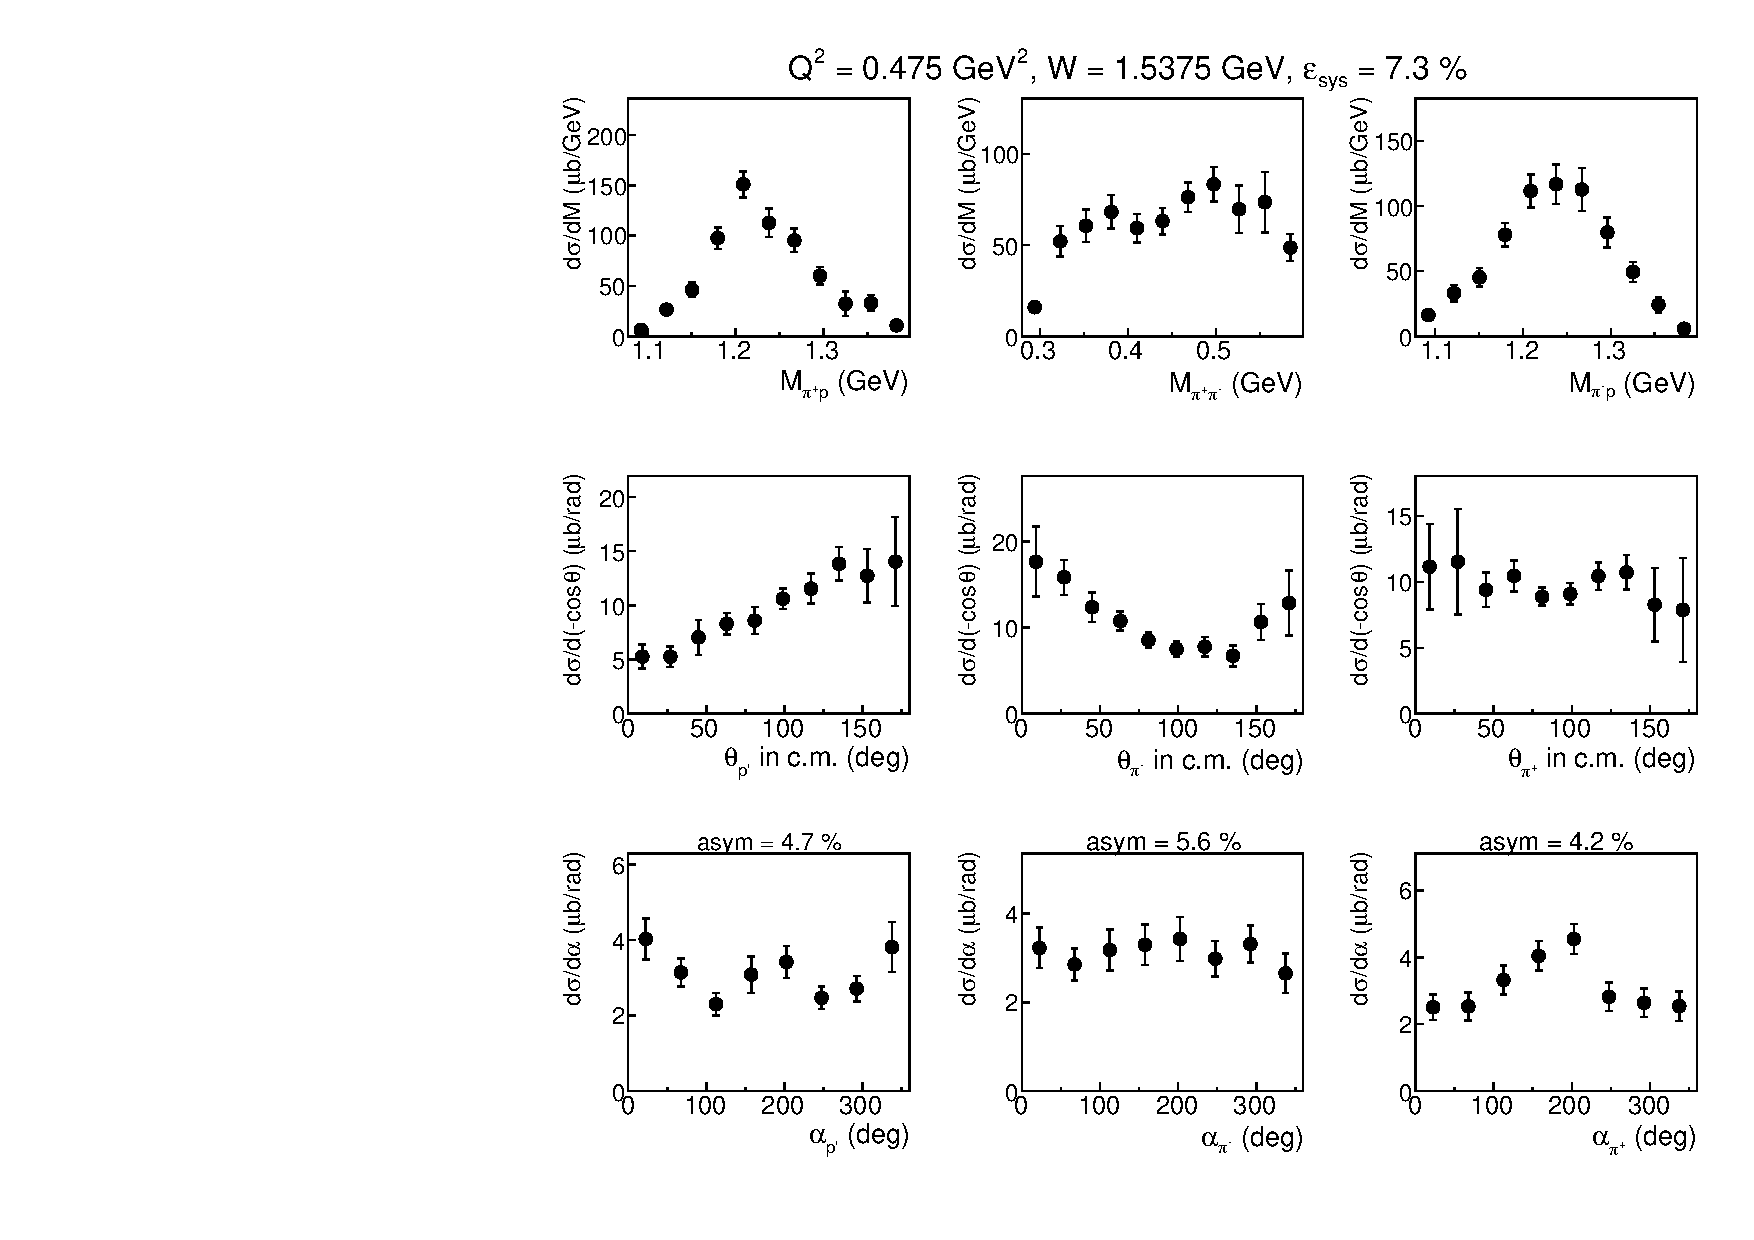
\includegraphics[width=0.45\textwidth]{pictures/appendix/1diff_distr/Q2_475/w_15375.pdf}}
\frame{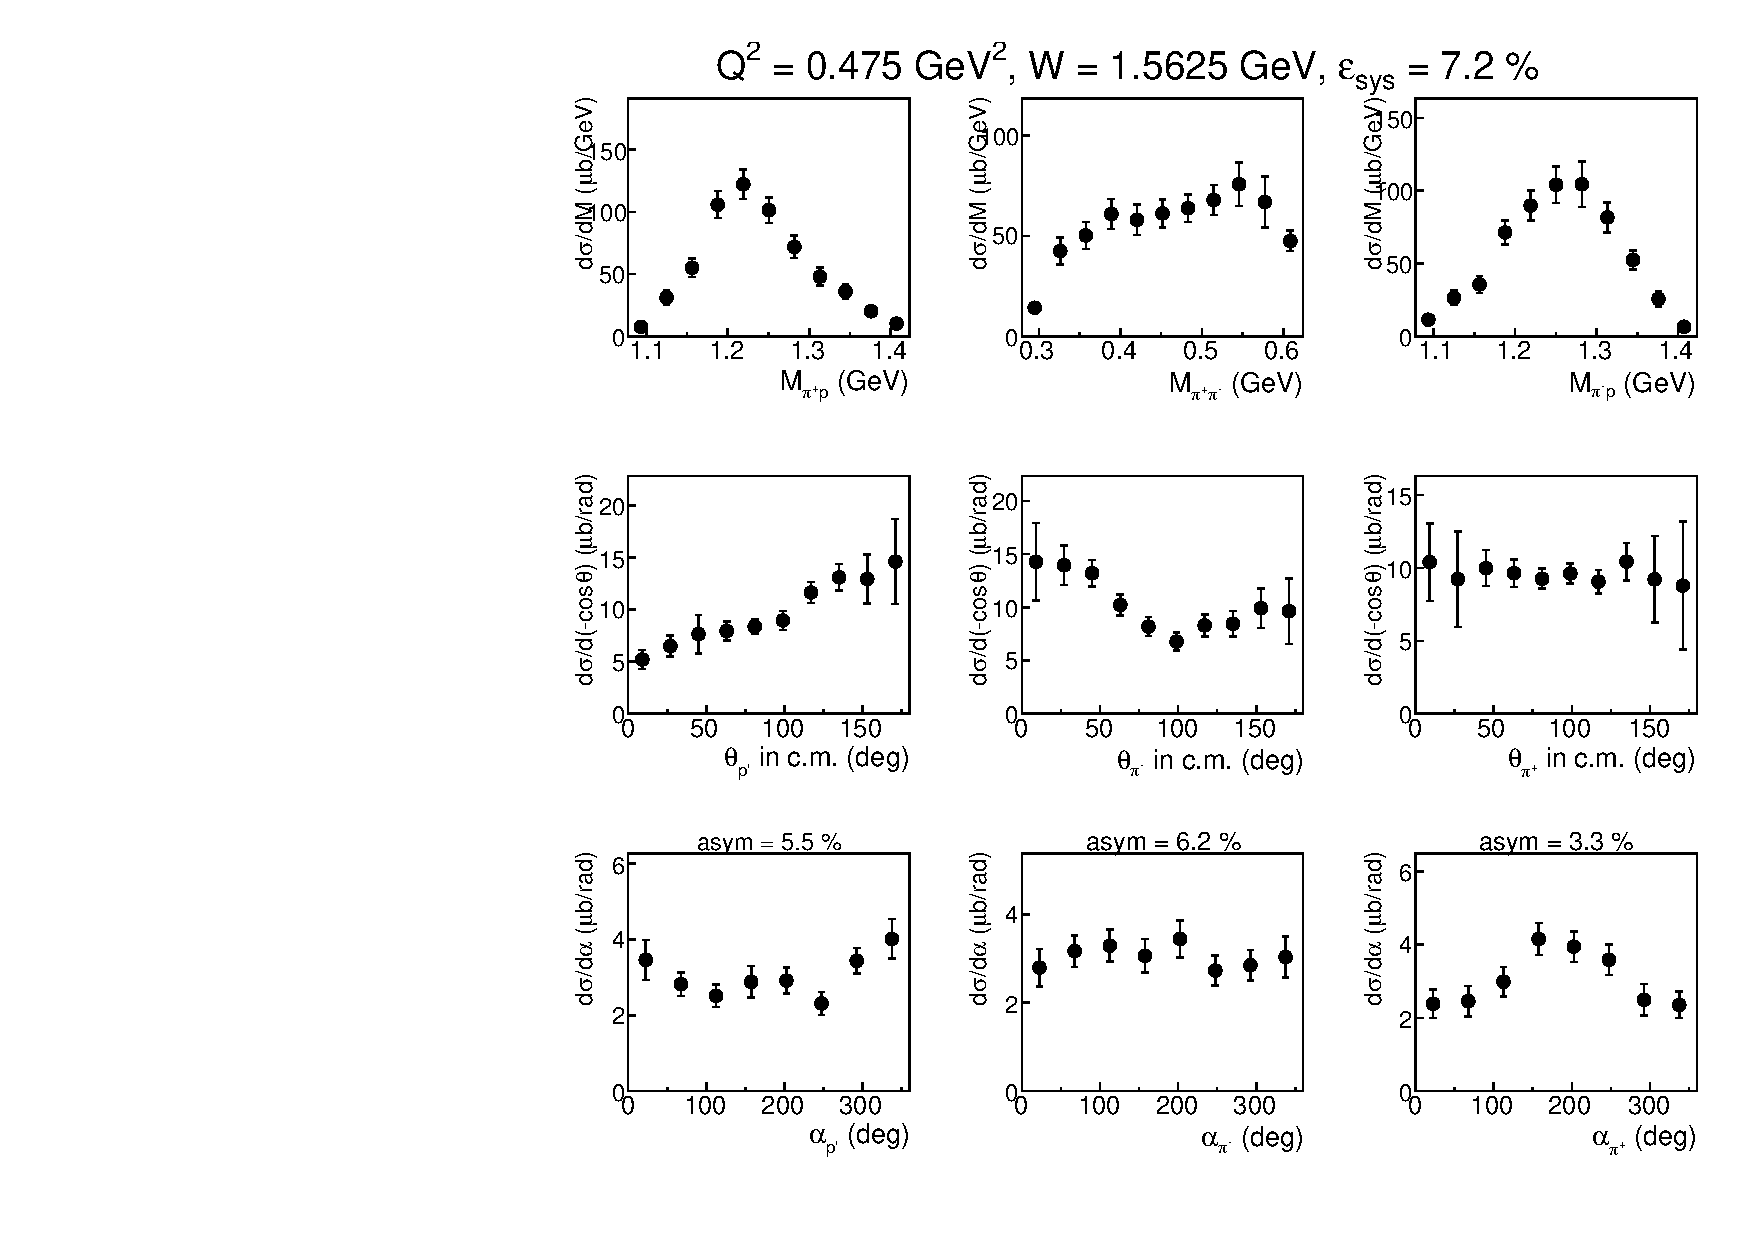
\includegraphics[width=0.45\textwidth]{pictures/appendix/1diff_distr/Q2_475/w_15625.pdf}}
\caption{\small } \label{fig:appx_5}
\end{center}
\end{figure}

\clearpage
\begin{figure}[htp]
\begin{center}
\frame{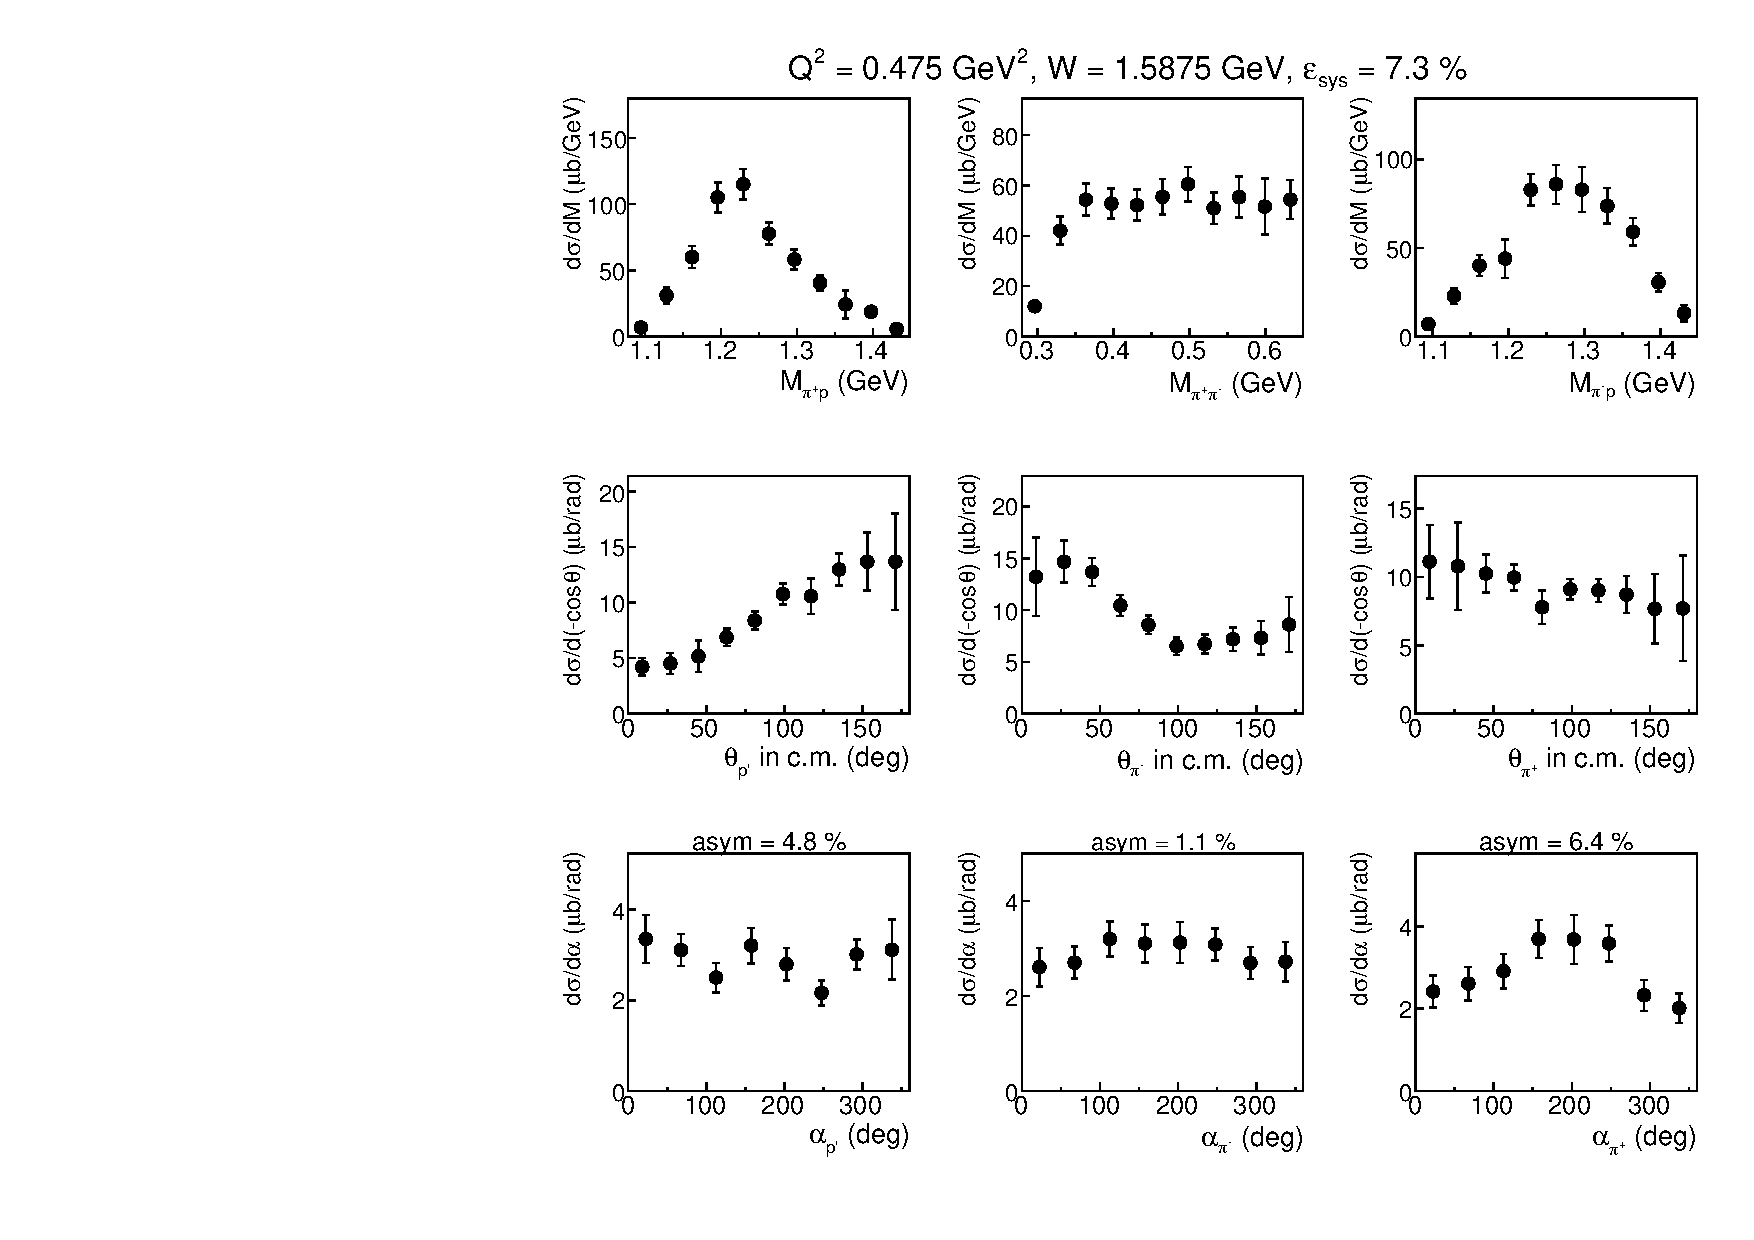
\includegraphics[width=0.45\textwidth]{pictures/appendix/1diff_distr/Q2_475/w_15875.pdf}}
\frame{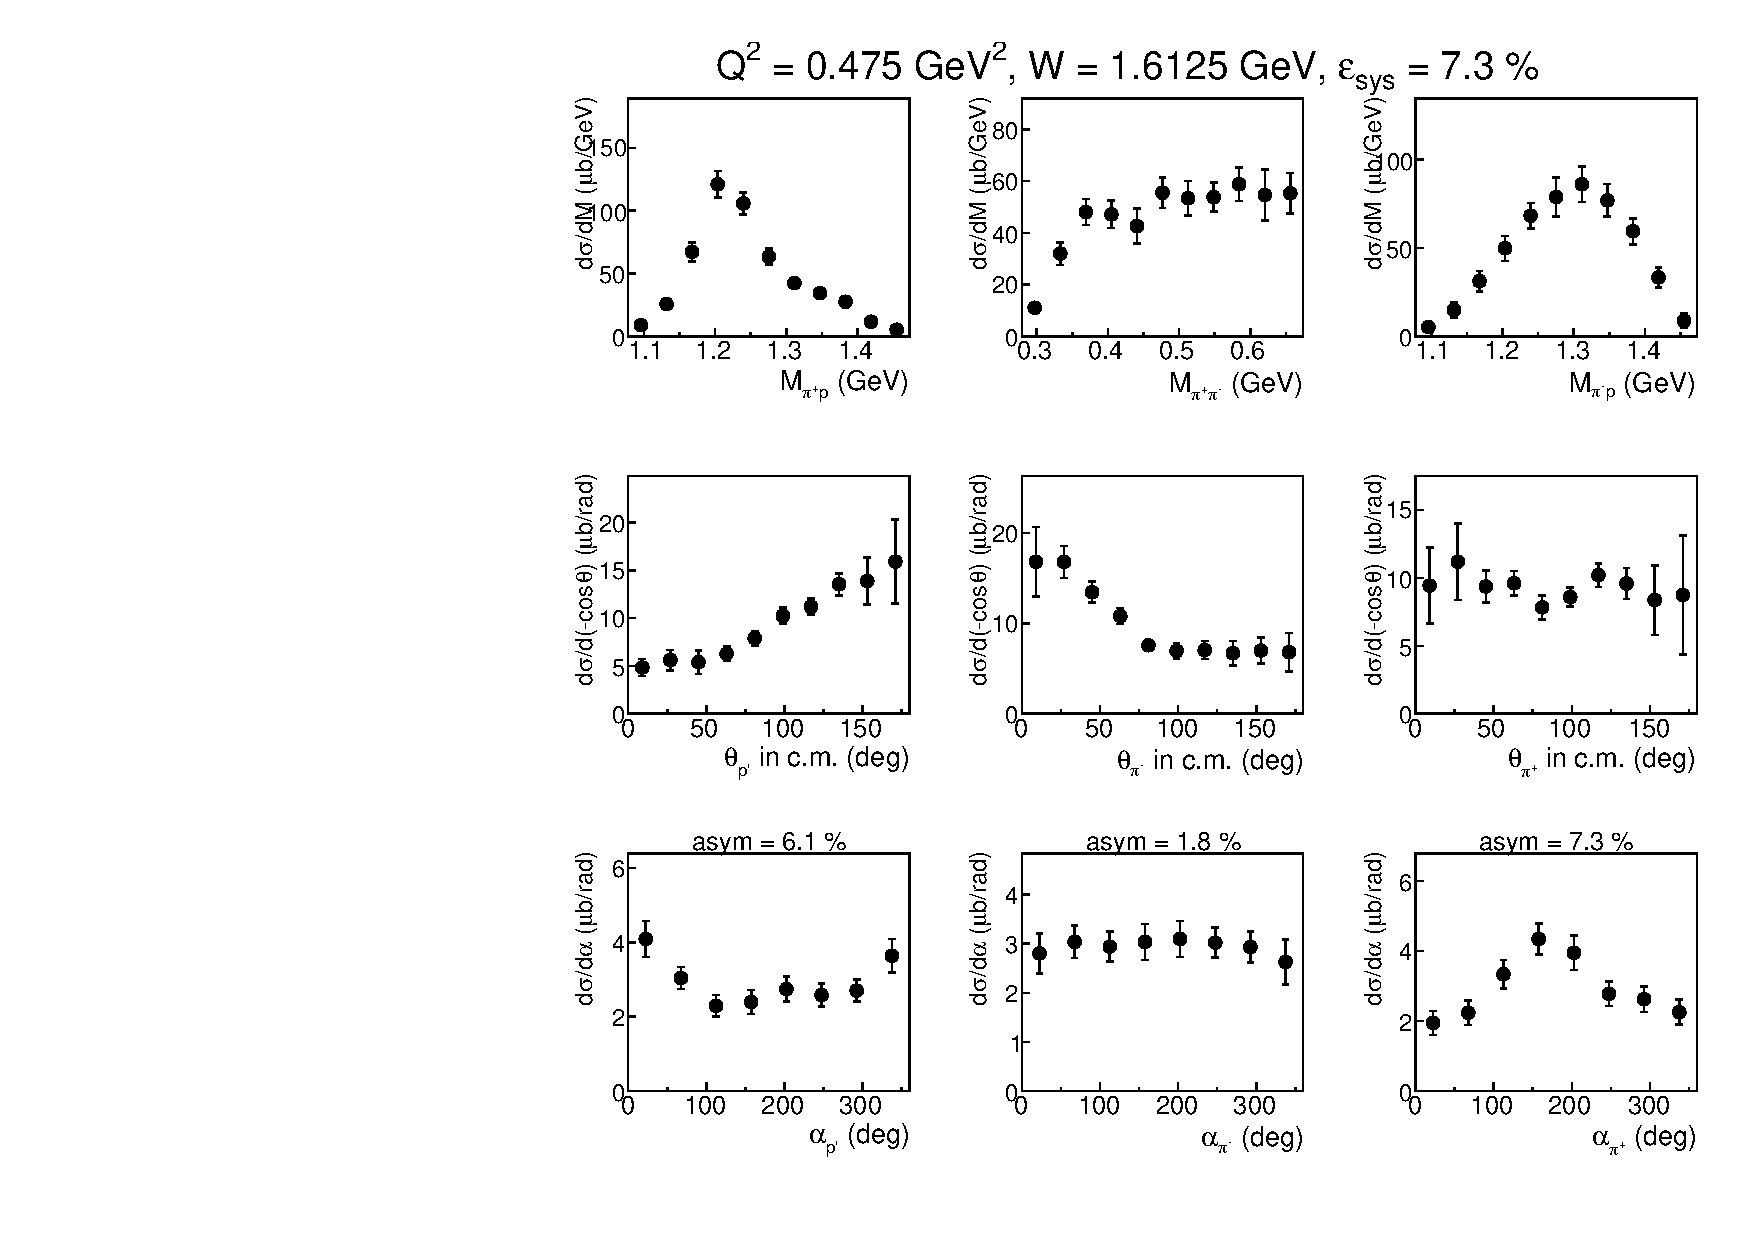
\includegraphics[width=0.45\textwidth]{pictures/appendix/1diff_distr/Q2_475/w_16125.pdf}}
\frame{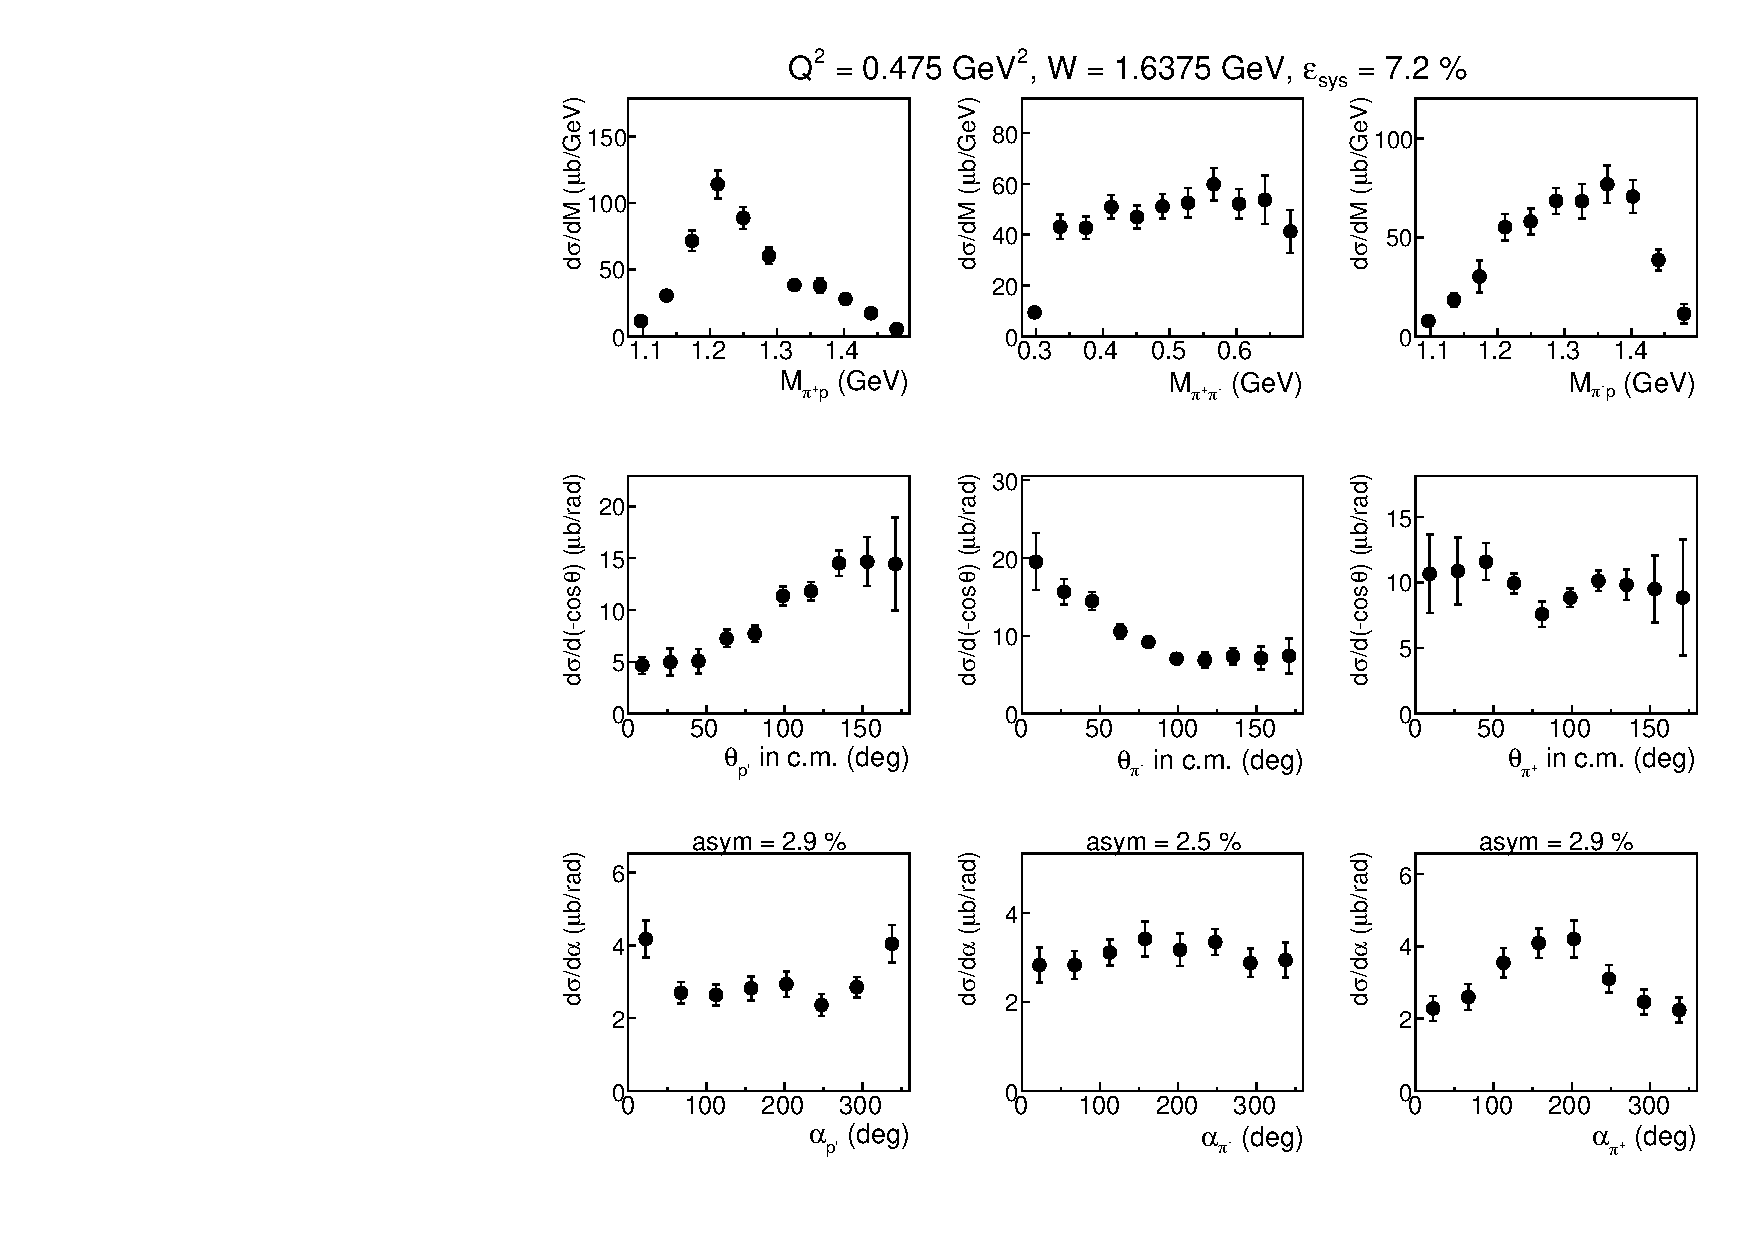
\includegraphics[width=0.45\textwidth]{pictures/appendix/1diff_distr/Q2_475/w_16375.pdf}}
\frame{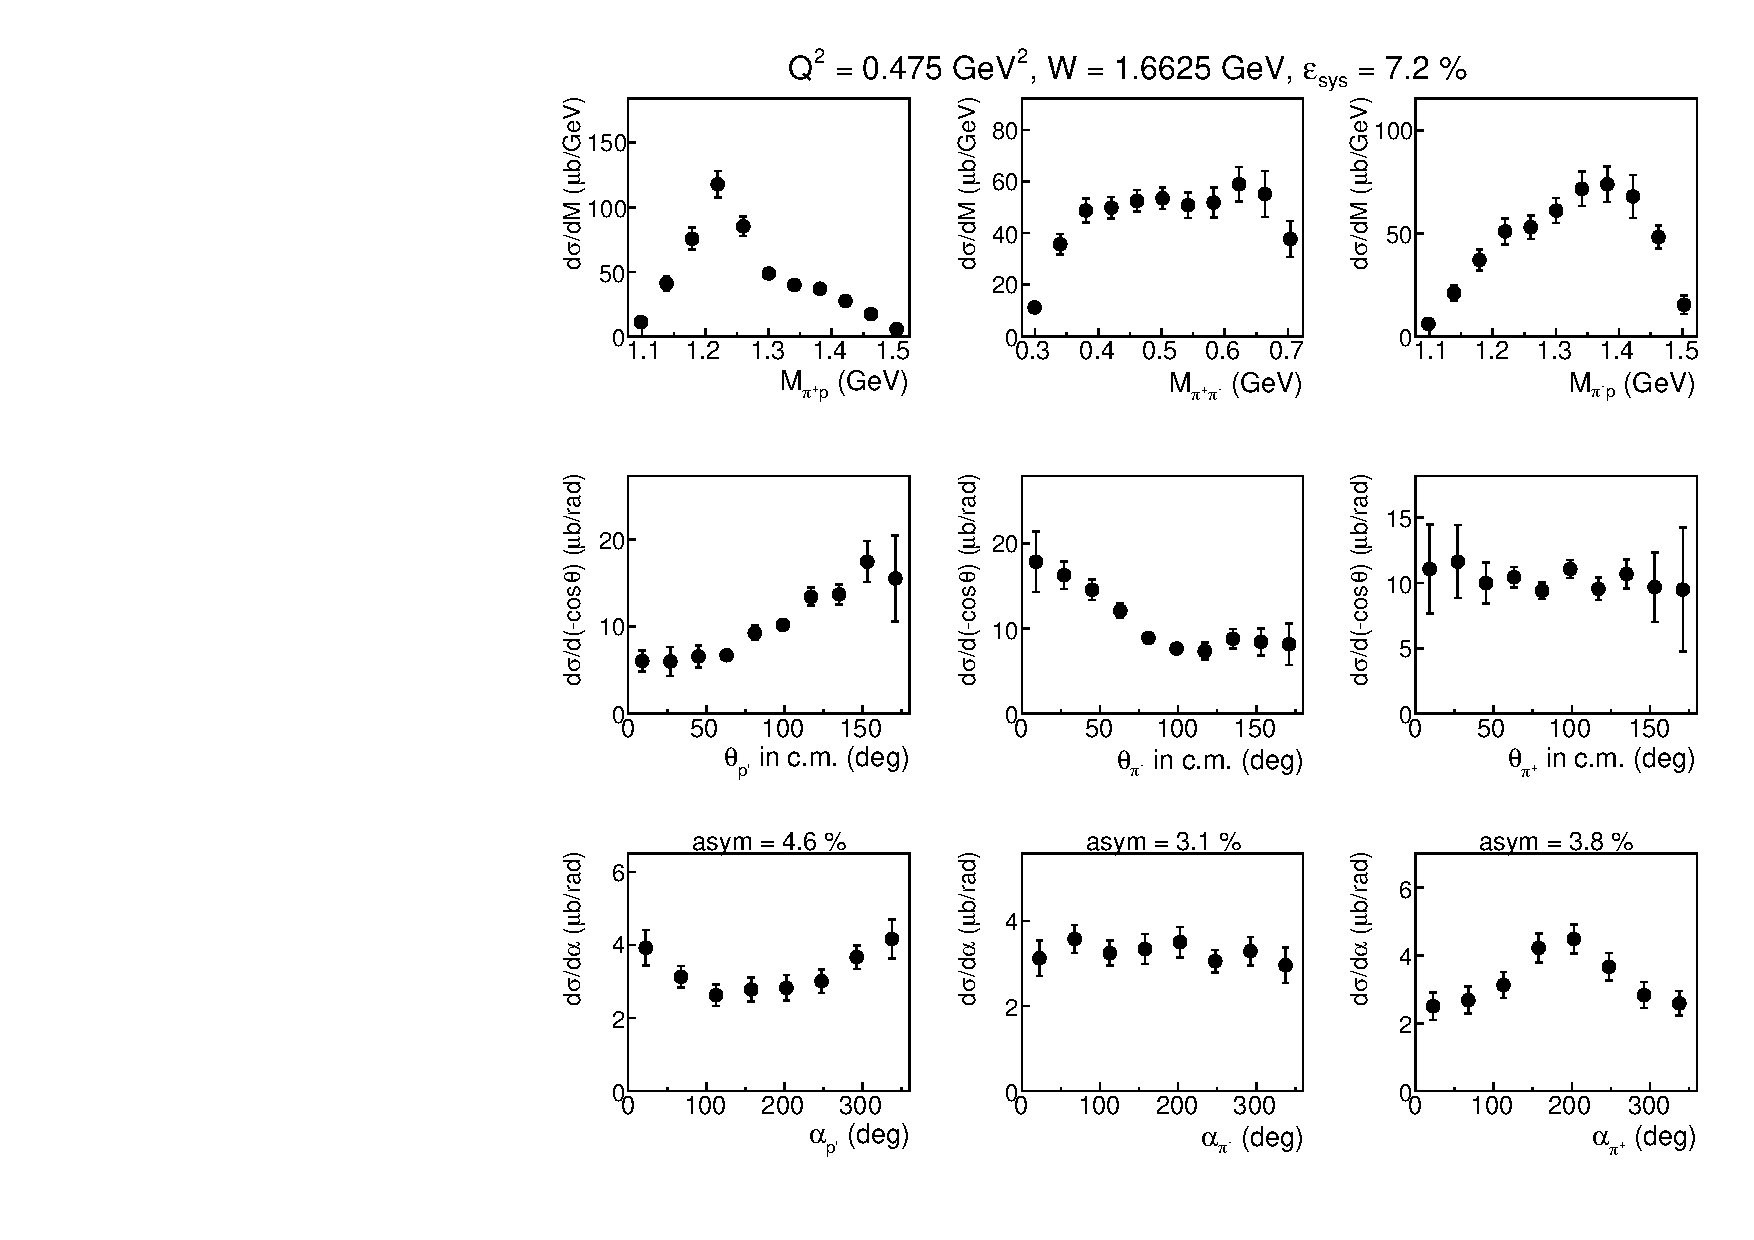
\includegraphics[width=0.45\textwidth]{pictures/appendix/1diff_distr/Q2_475/w_16625.pdf}}
\caption{\small } \label{fig:appx_6}
\end{center}
\end{figure}

\clearpage
\begin{figure}[htp]
\begin{center}
\frame{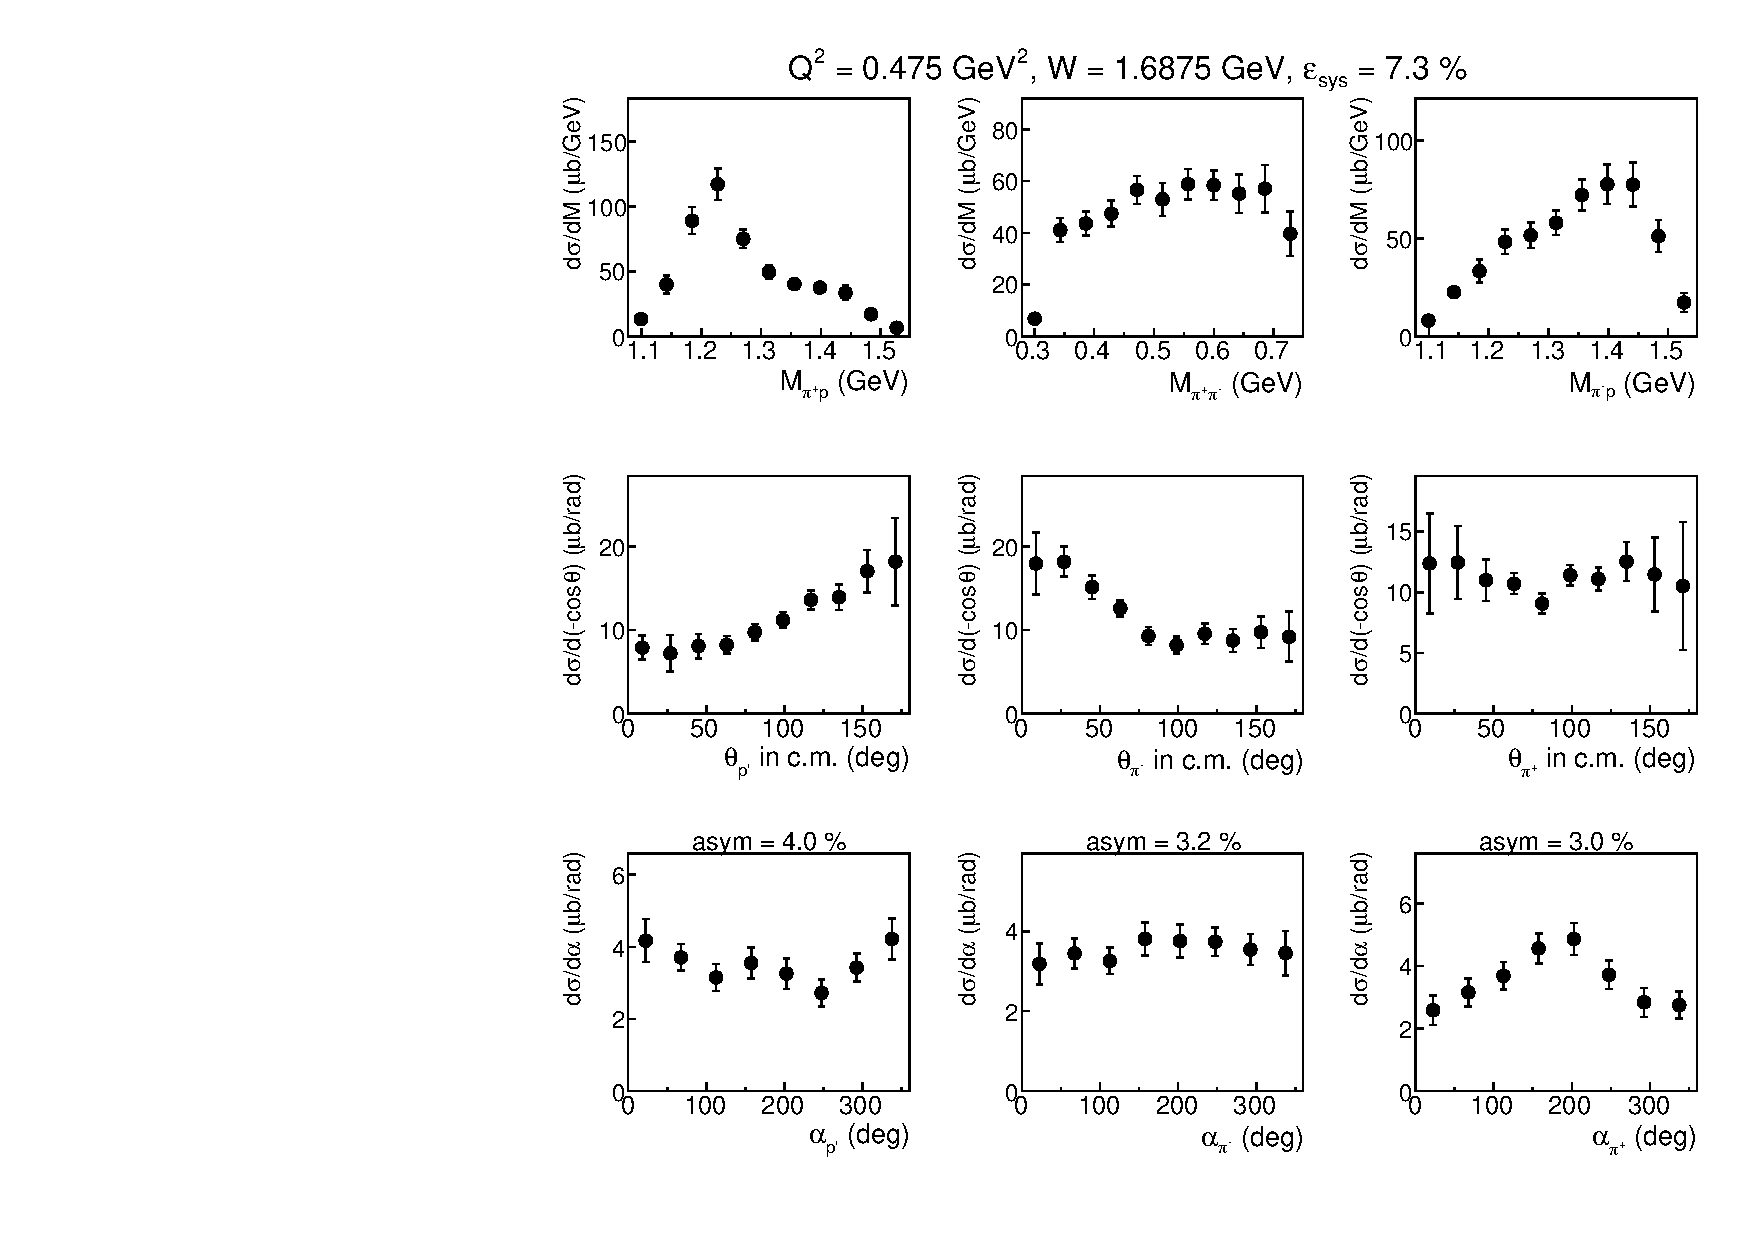
\includegraphics[width=0.45\textwidth]{pictures/appendix/1diff_distr/Q2_475/w_16875.pdf}}
\frame{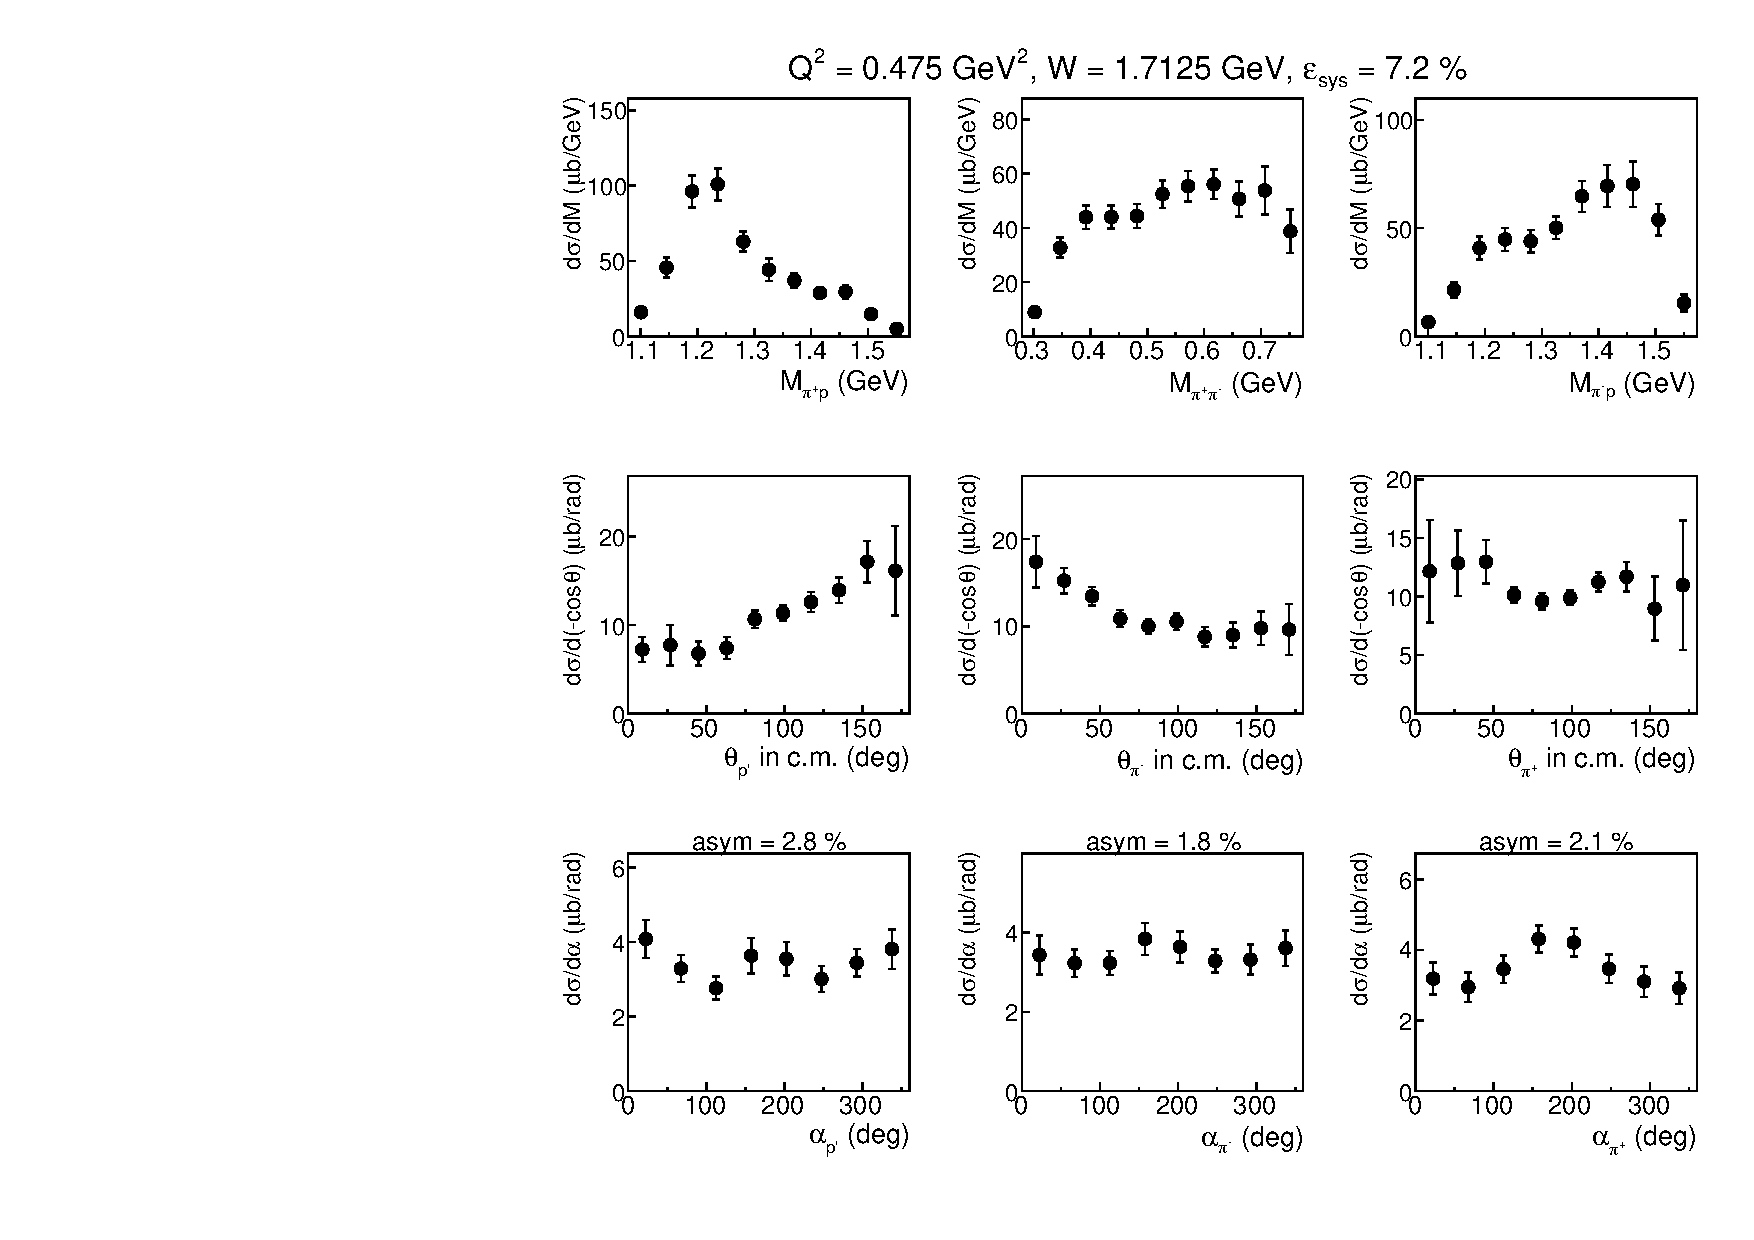
\includegraphics[width=0.45\textwidth]{pictures/appendix/1diff_distr/Q2_475/w_17125.pdf}}
\frame{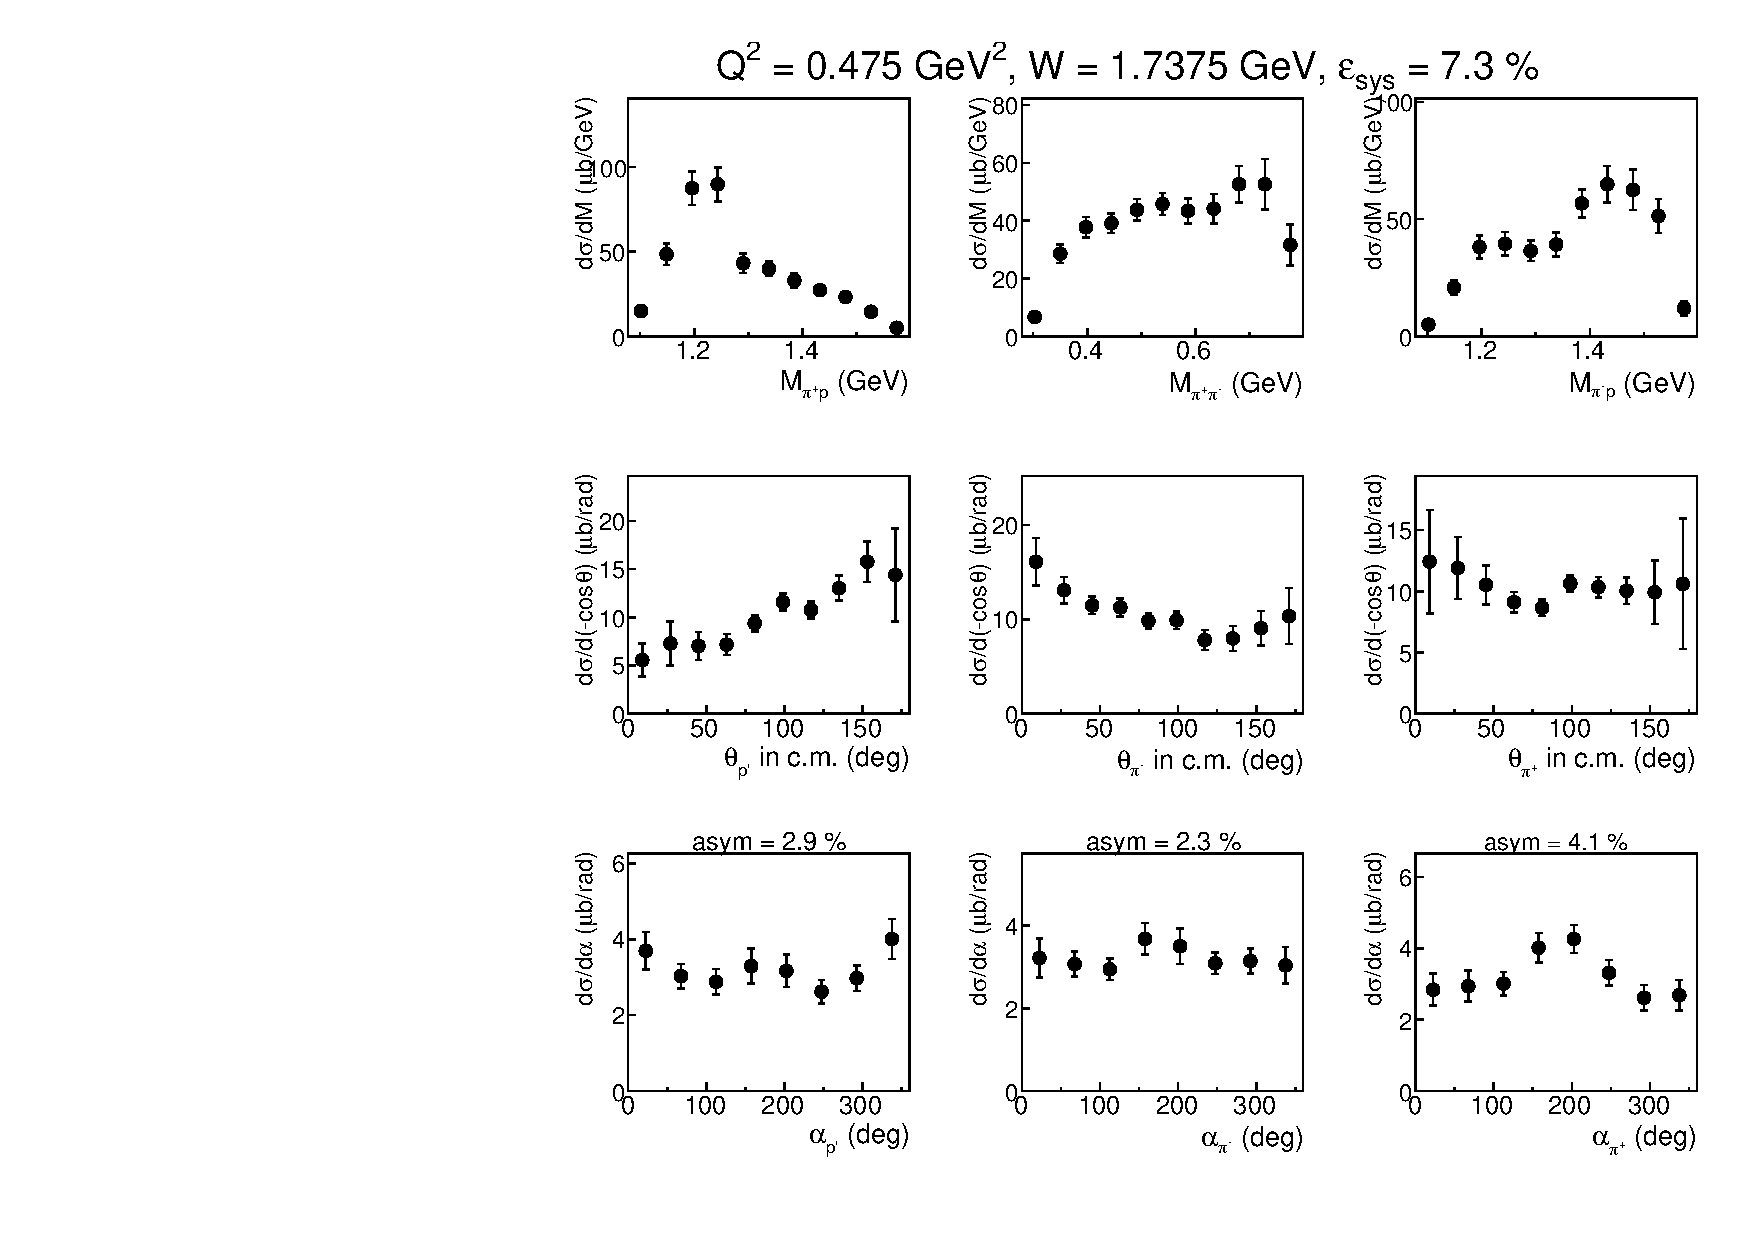
\includegraphics[width=0.45\textwidth]{pictures/appendix/1diff_distr/Q2_475/w_17375.pdf}}
\frame{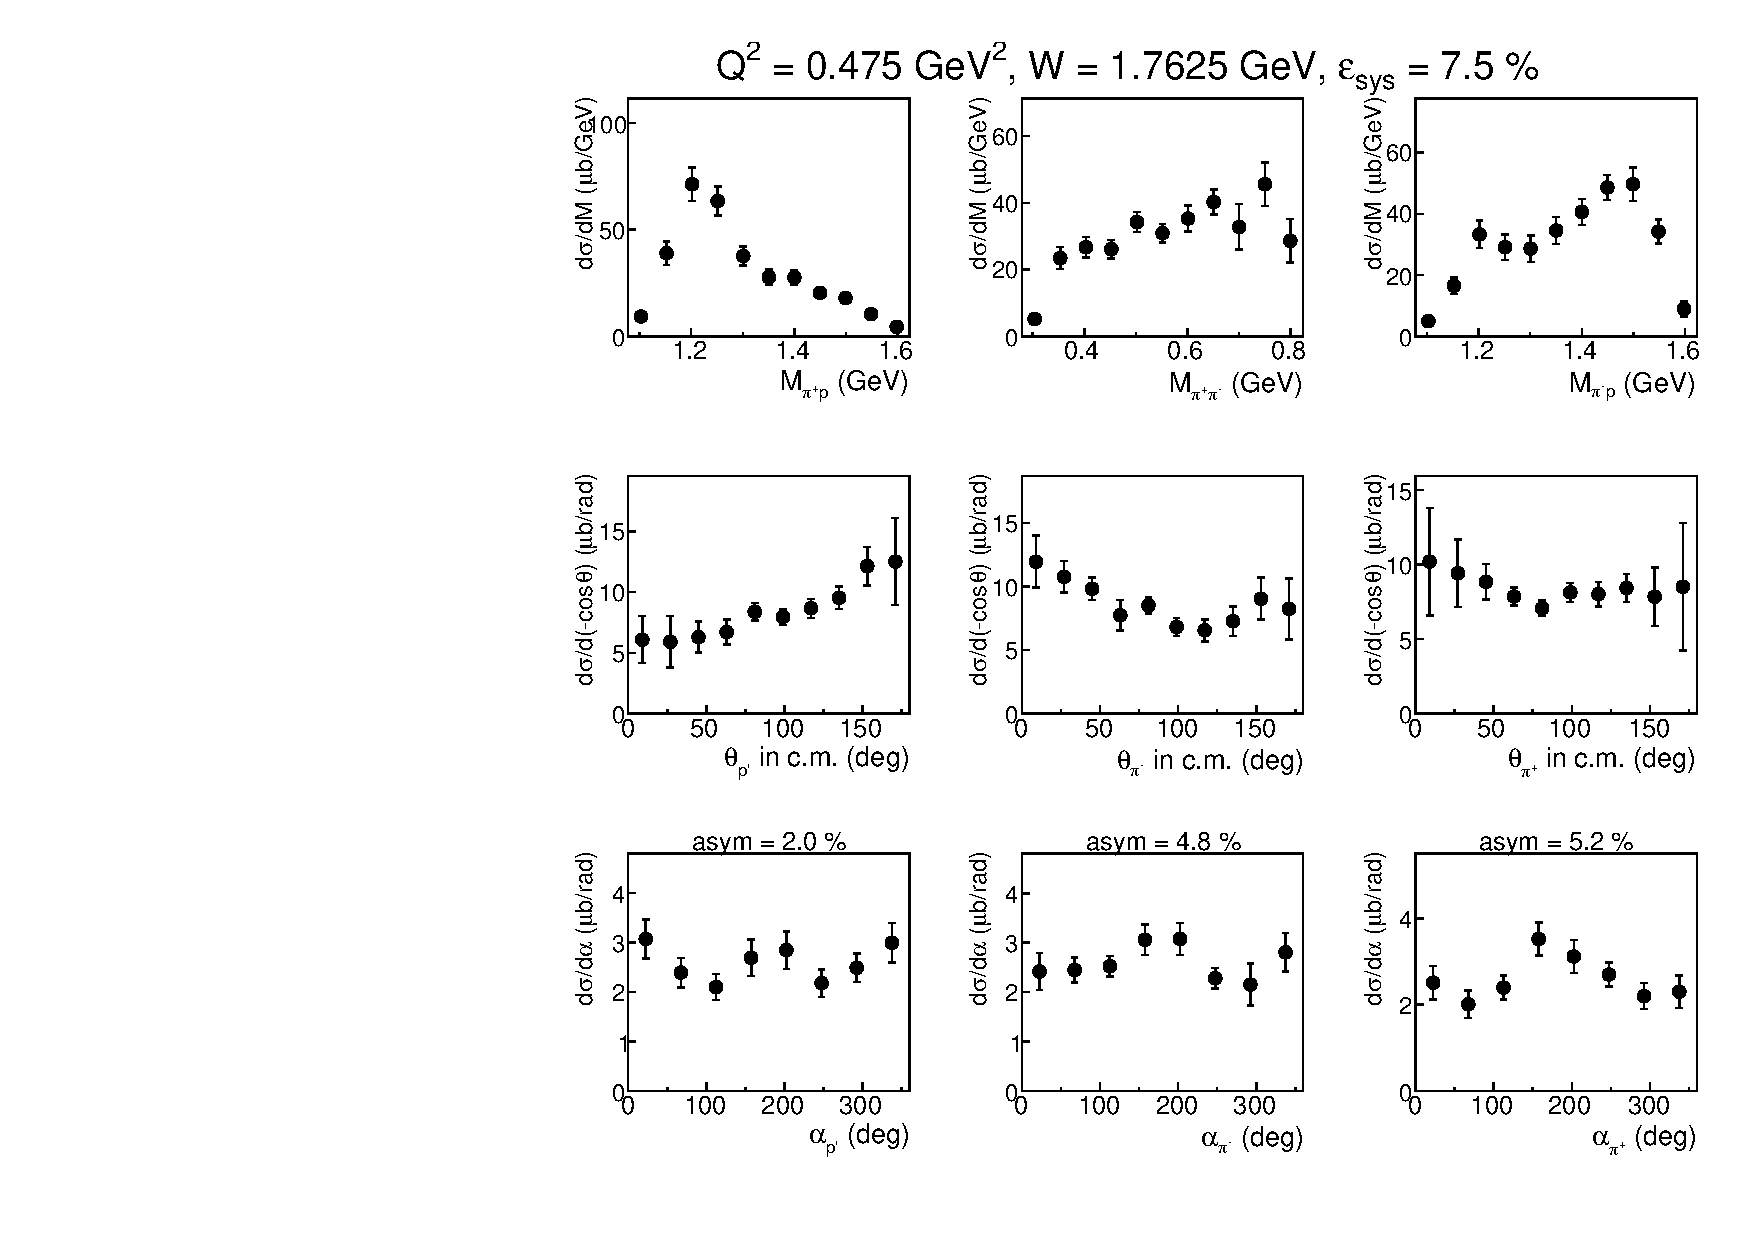
\includegraphics[width=0.45\textwidth]{pictures/appendix/1diff_distr/Q2_475/w_17625.pdf}}
\caption{\small } \label{fig:appx_7}
\end{center}
\end{figure}

\clearpage
\begin{figure}[htp]
\begin{center}
\frame{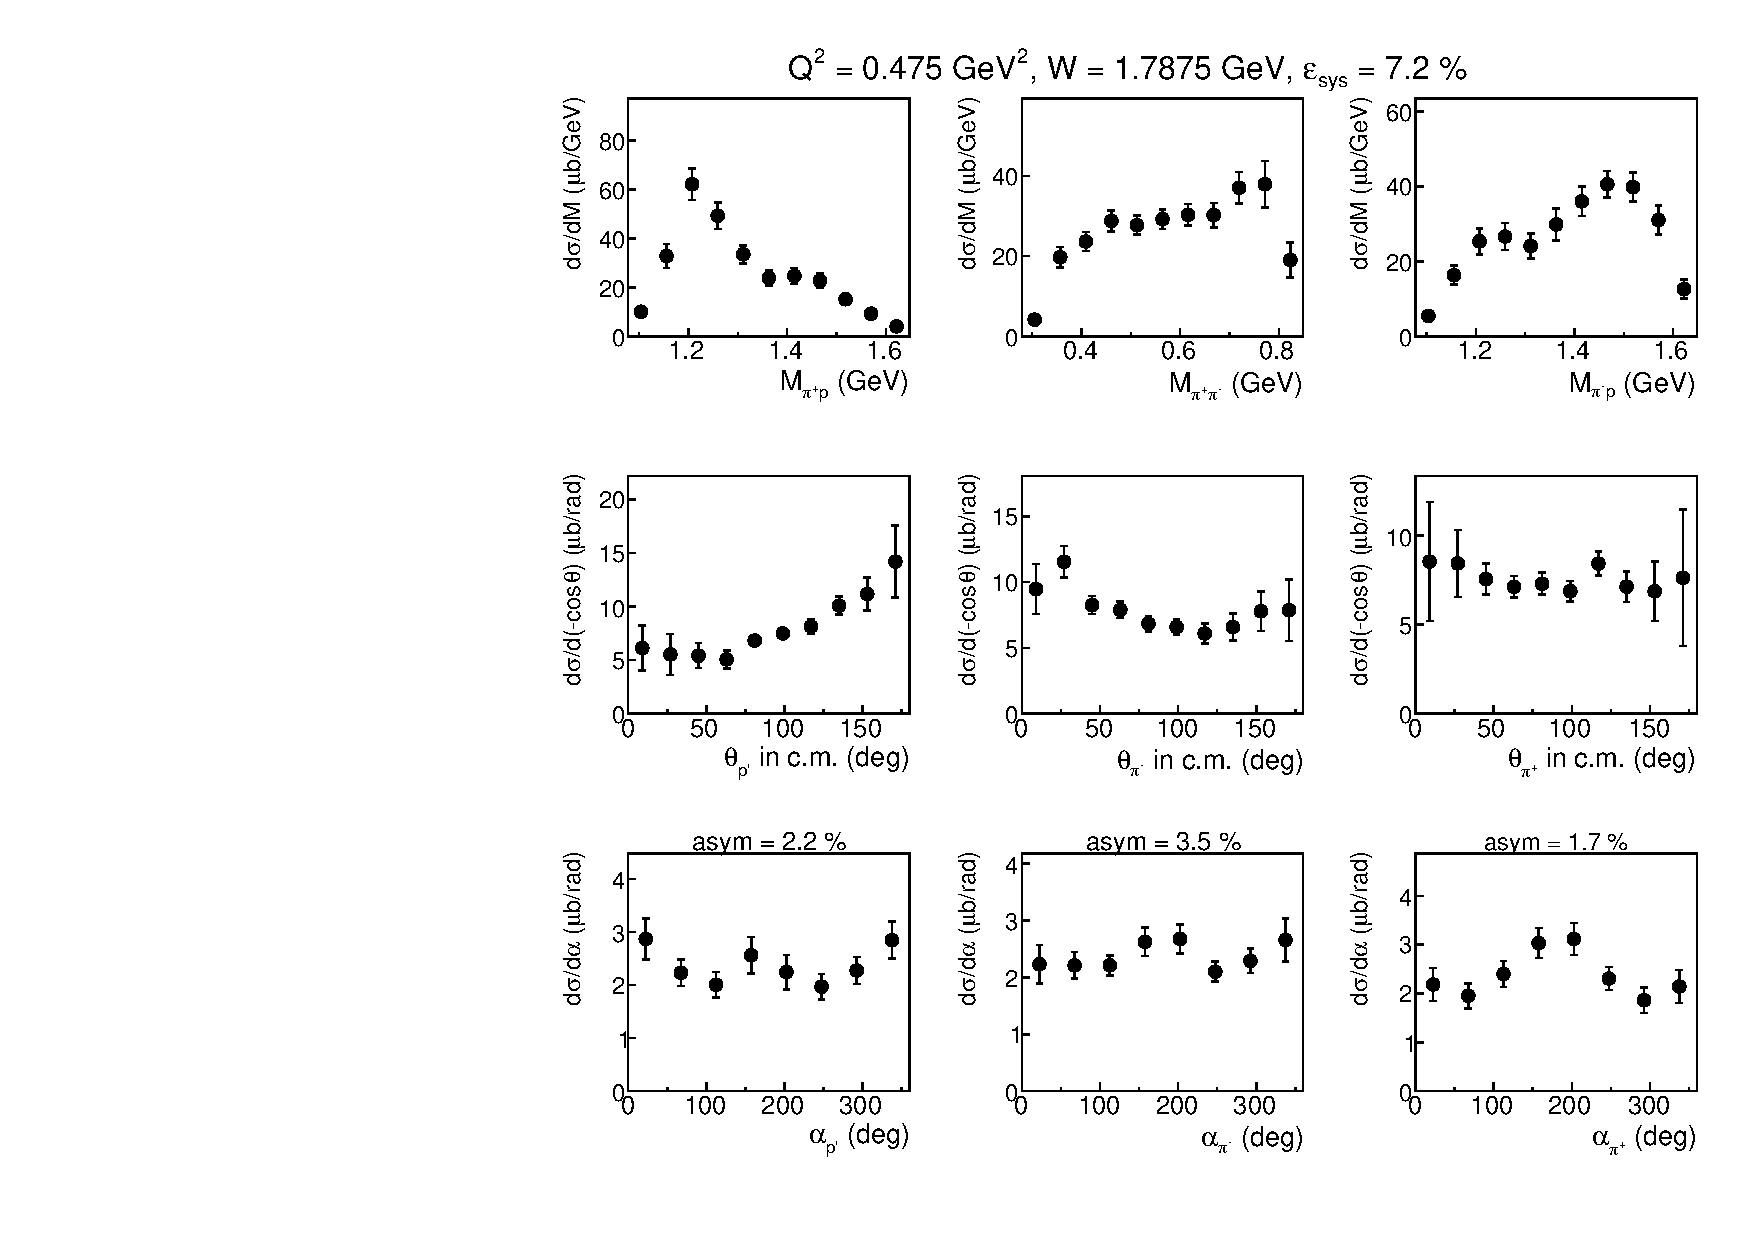
\includegraphics[width=0.45\textwidth]{pictures/appendix/1diff_distr/Q2_475/w_17875.pdf}}
\frame{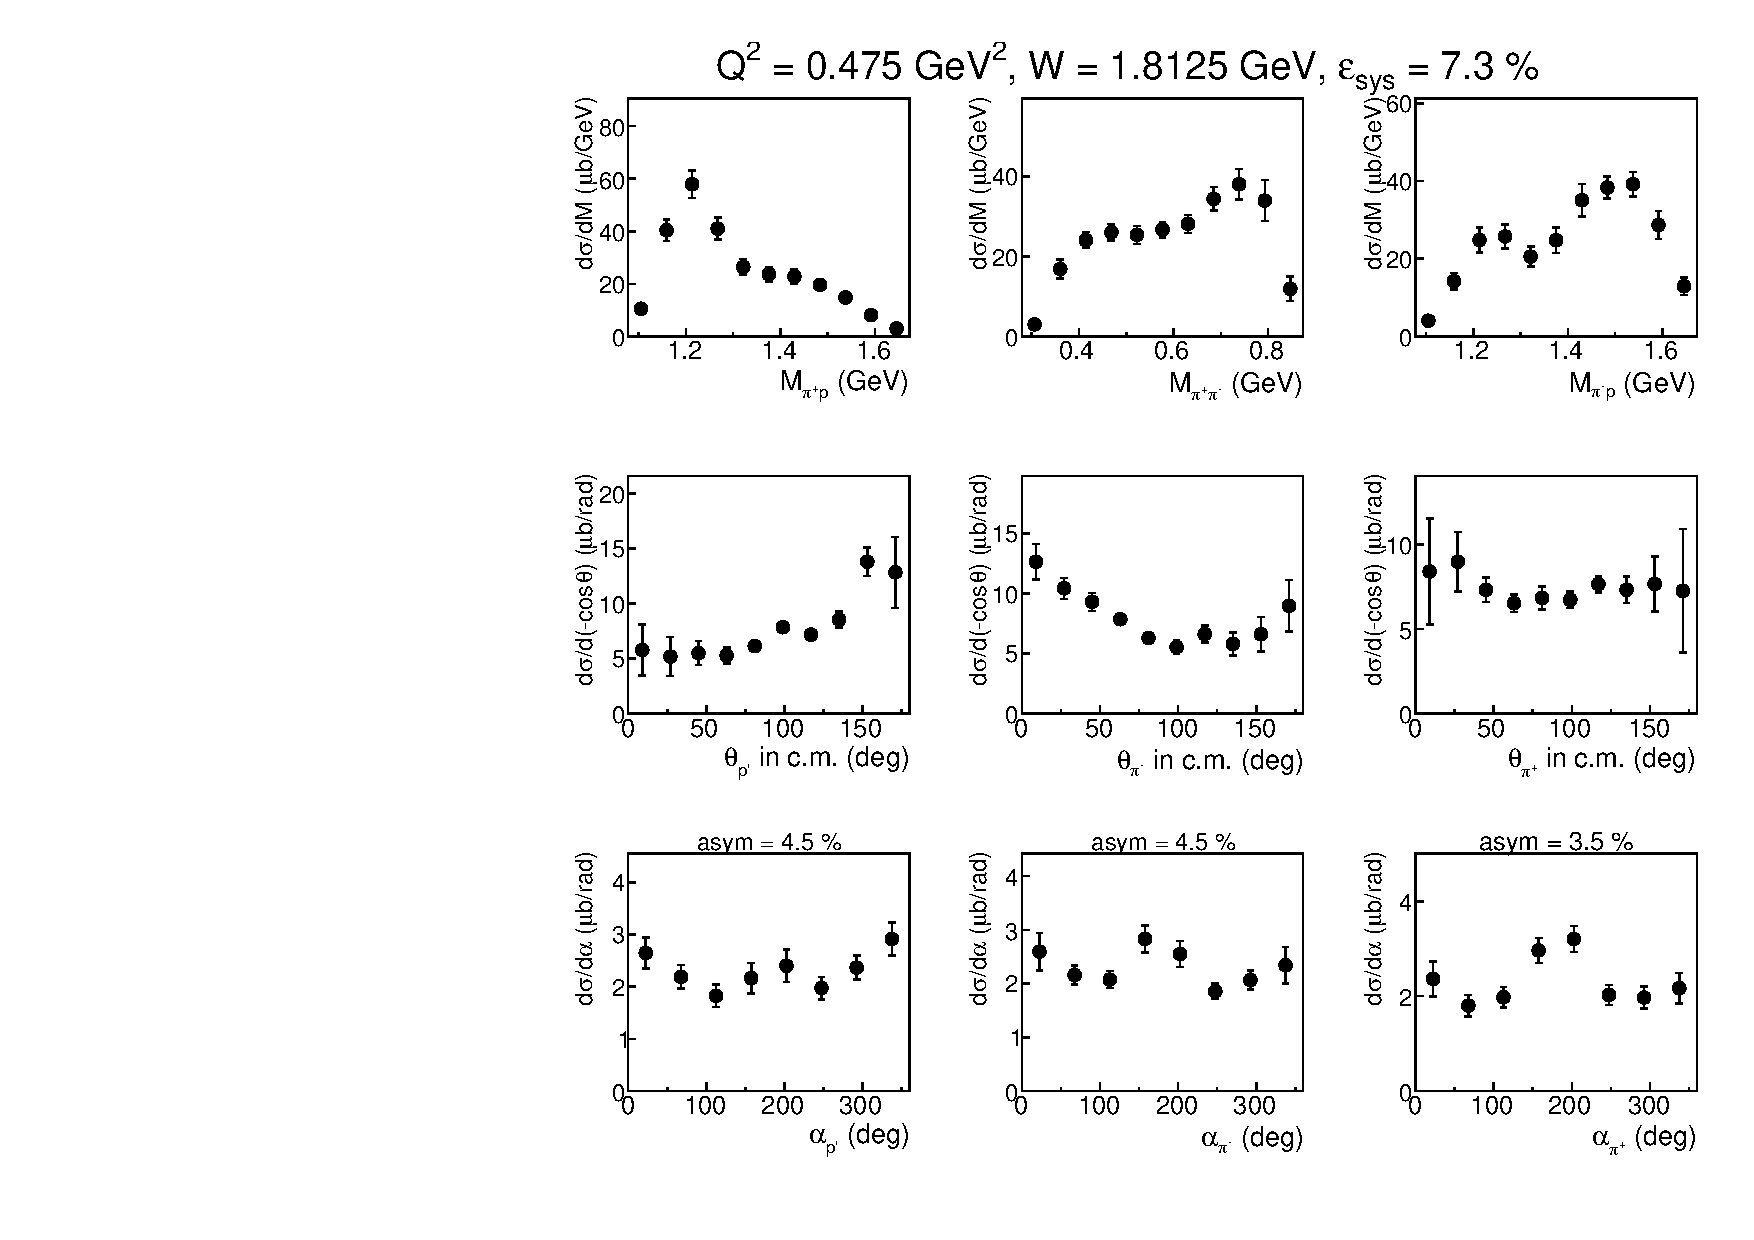
\includegraphics[width=0.45\textwidth]{pictures/appendix/1diff_distr/Q2_475/w_18125.pdf}}
\frame{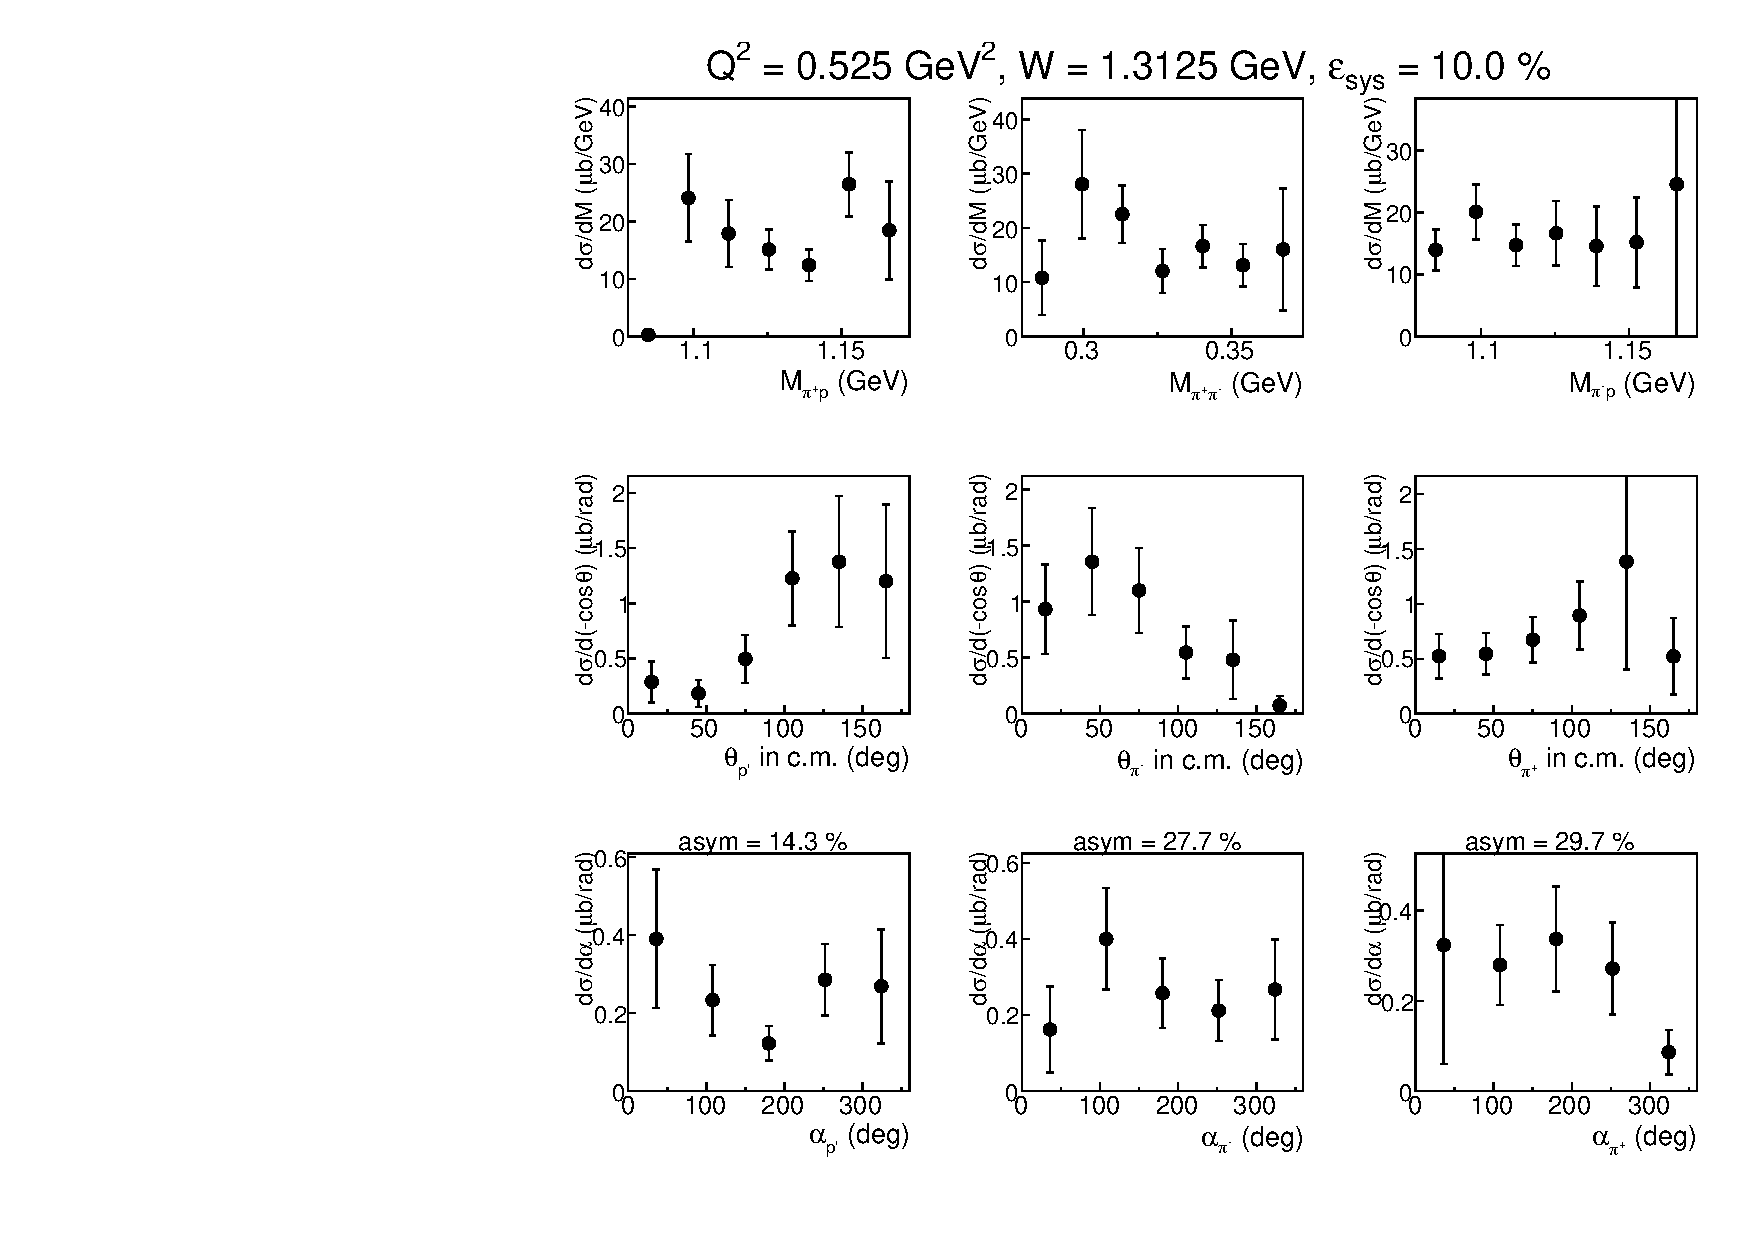
\includegraphics[width=0.45\textwidth]{pictures/appendix/1diff_distr/Q2_525/w_13125.pdf}}
\frame{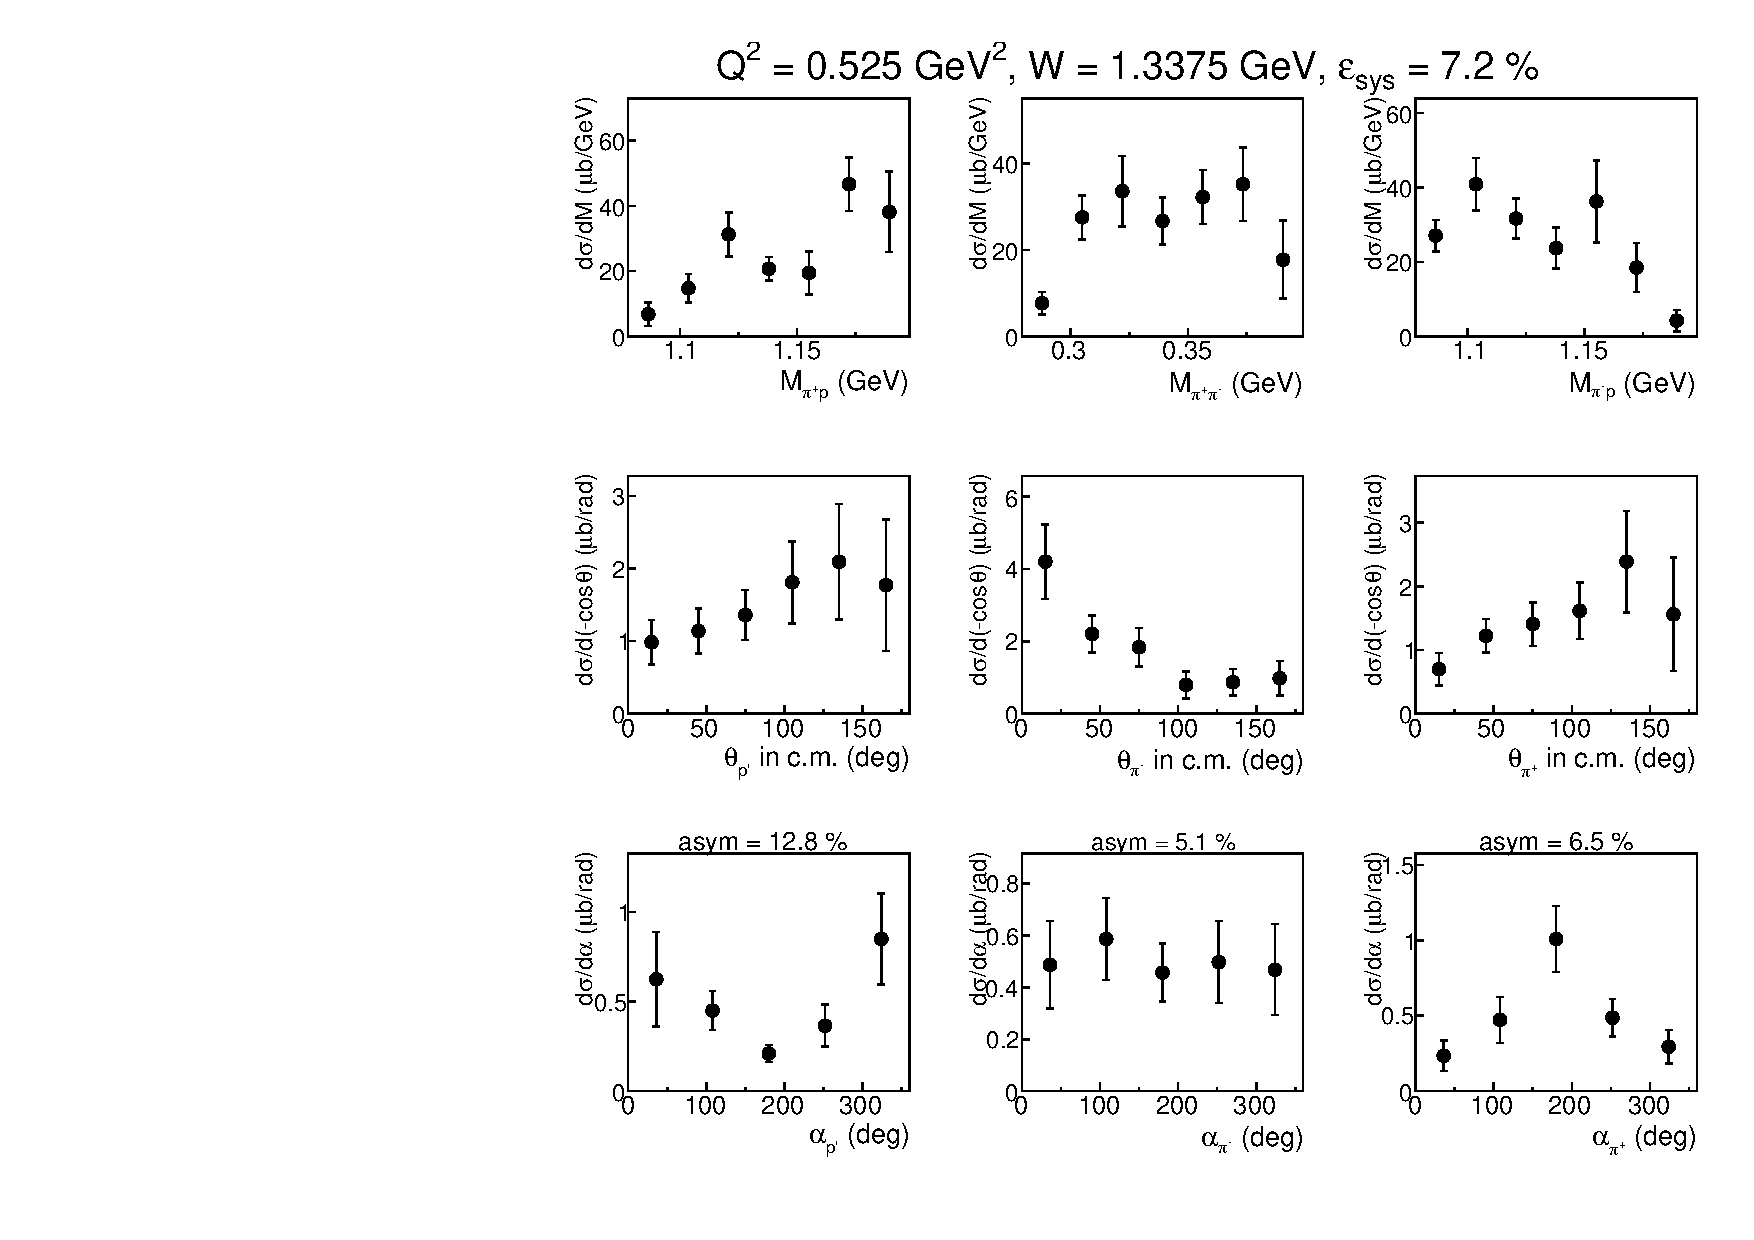
\includegraphics[width=0.45\textwidth]{pictures/appendix/1diff_distr/Q2_525/w_13375.pdf}}
\caption{\small } \label{fig:appx_8}
\end{center}
\end{figure}

\clearpage
\begin{figure}[htp]
\begin{center}
\frame{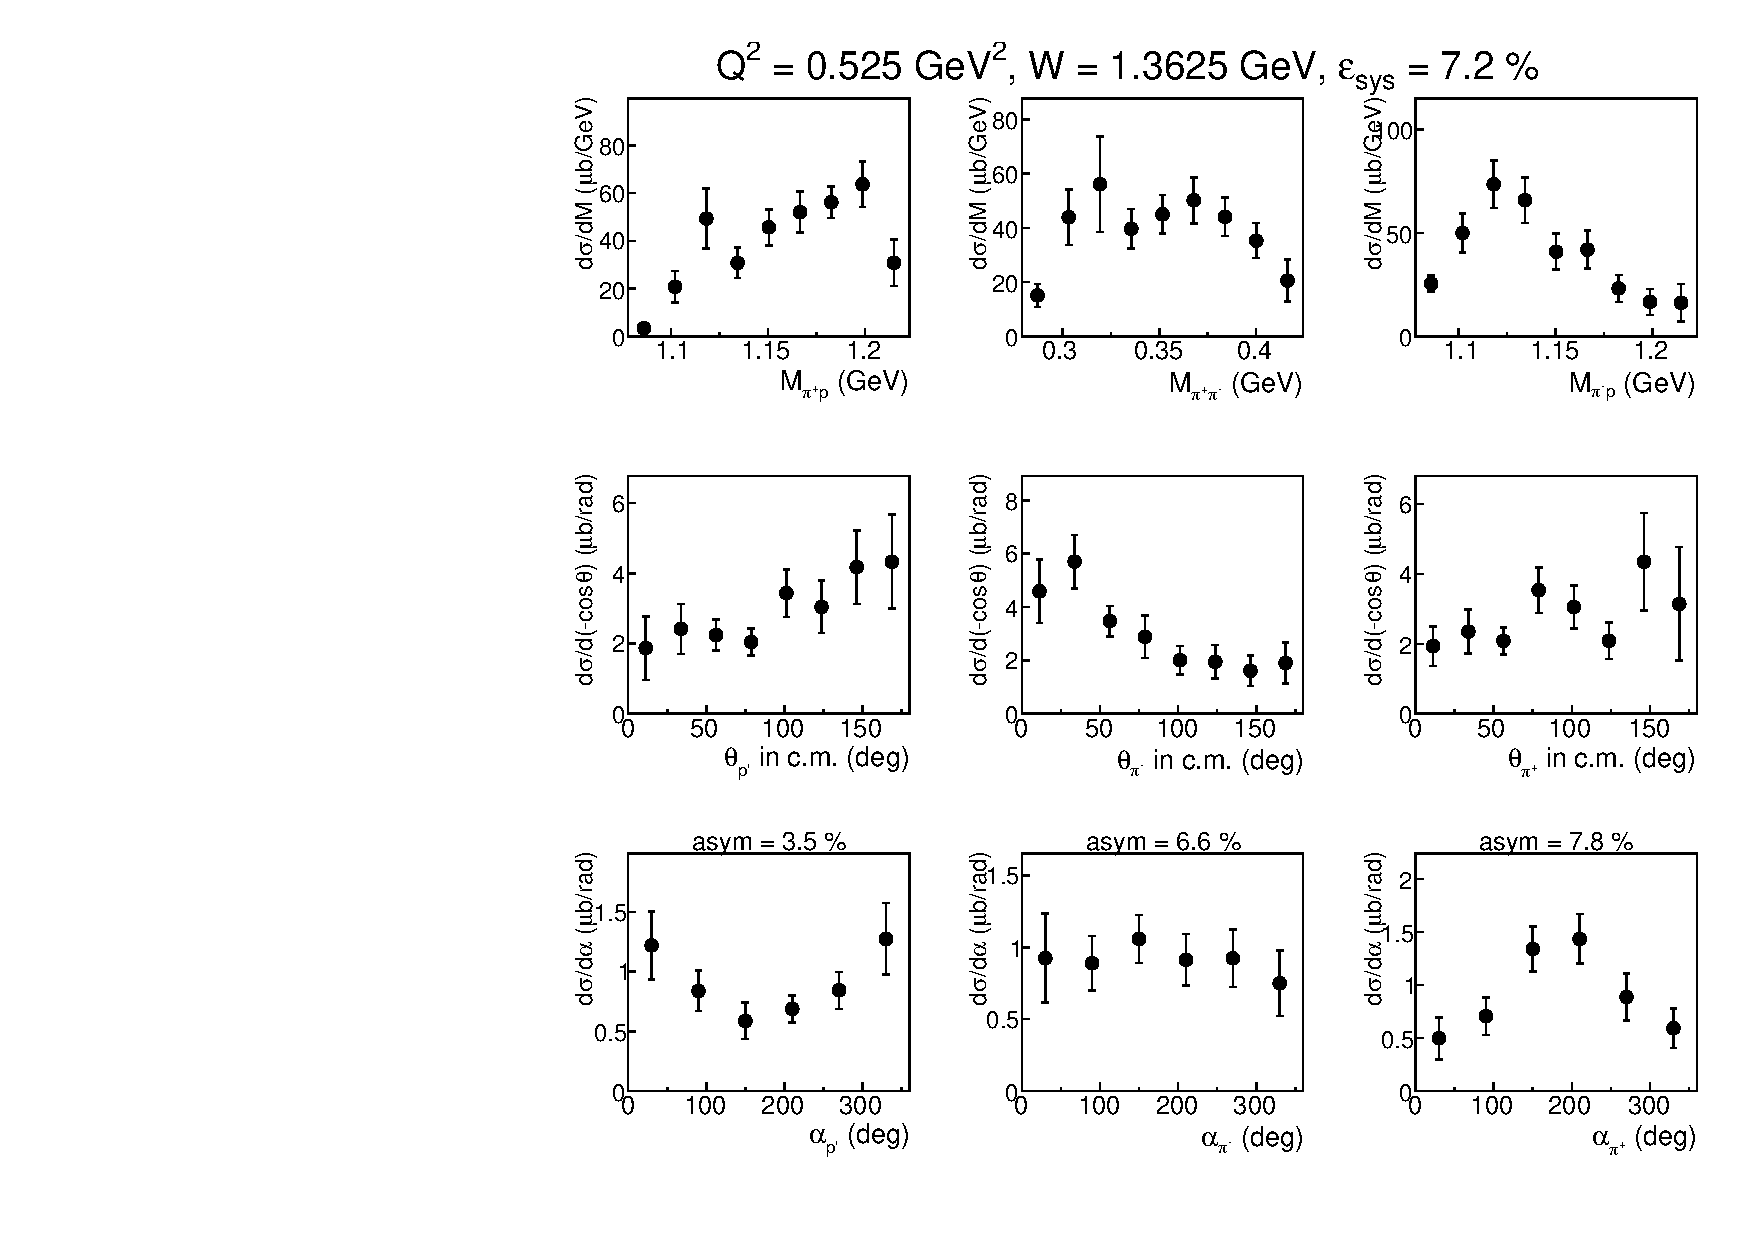
\includegraphics[width=0.45\textwidth]{pictures/appendix/1diff_distr/Q2_525/w_13625.pdf}}
\frame{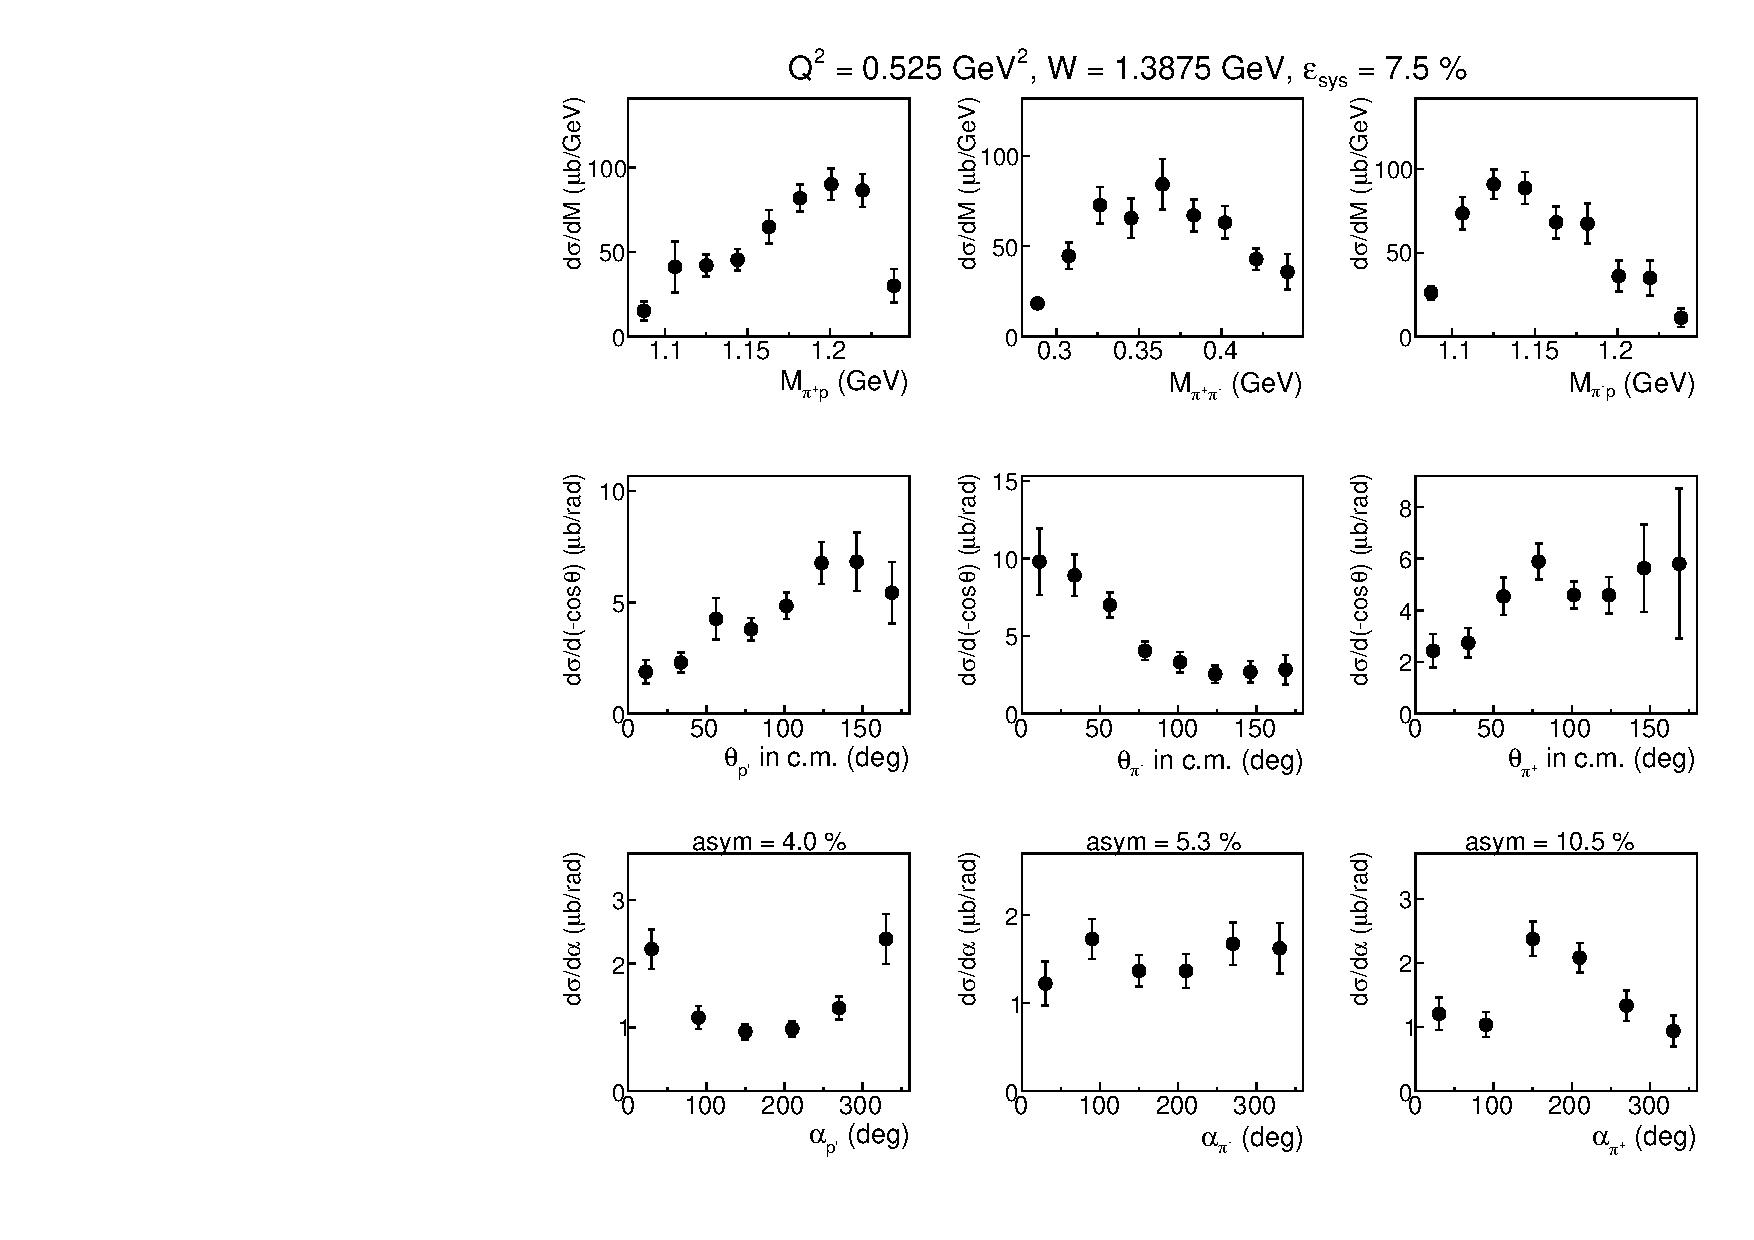
\includegraphics[width=0.45\textwidth]{pictures/appendix/1diff_distr/Q2_525/w_13875.pdf}}
\frame{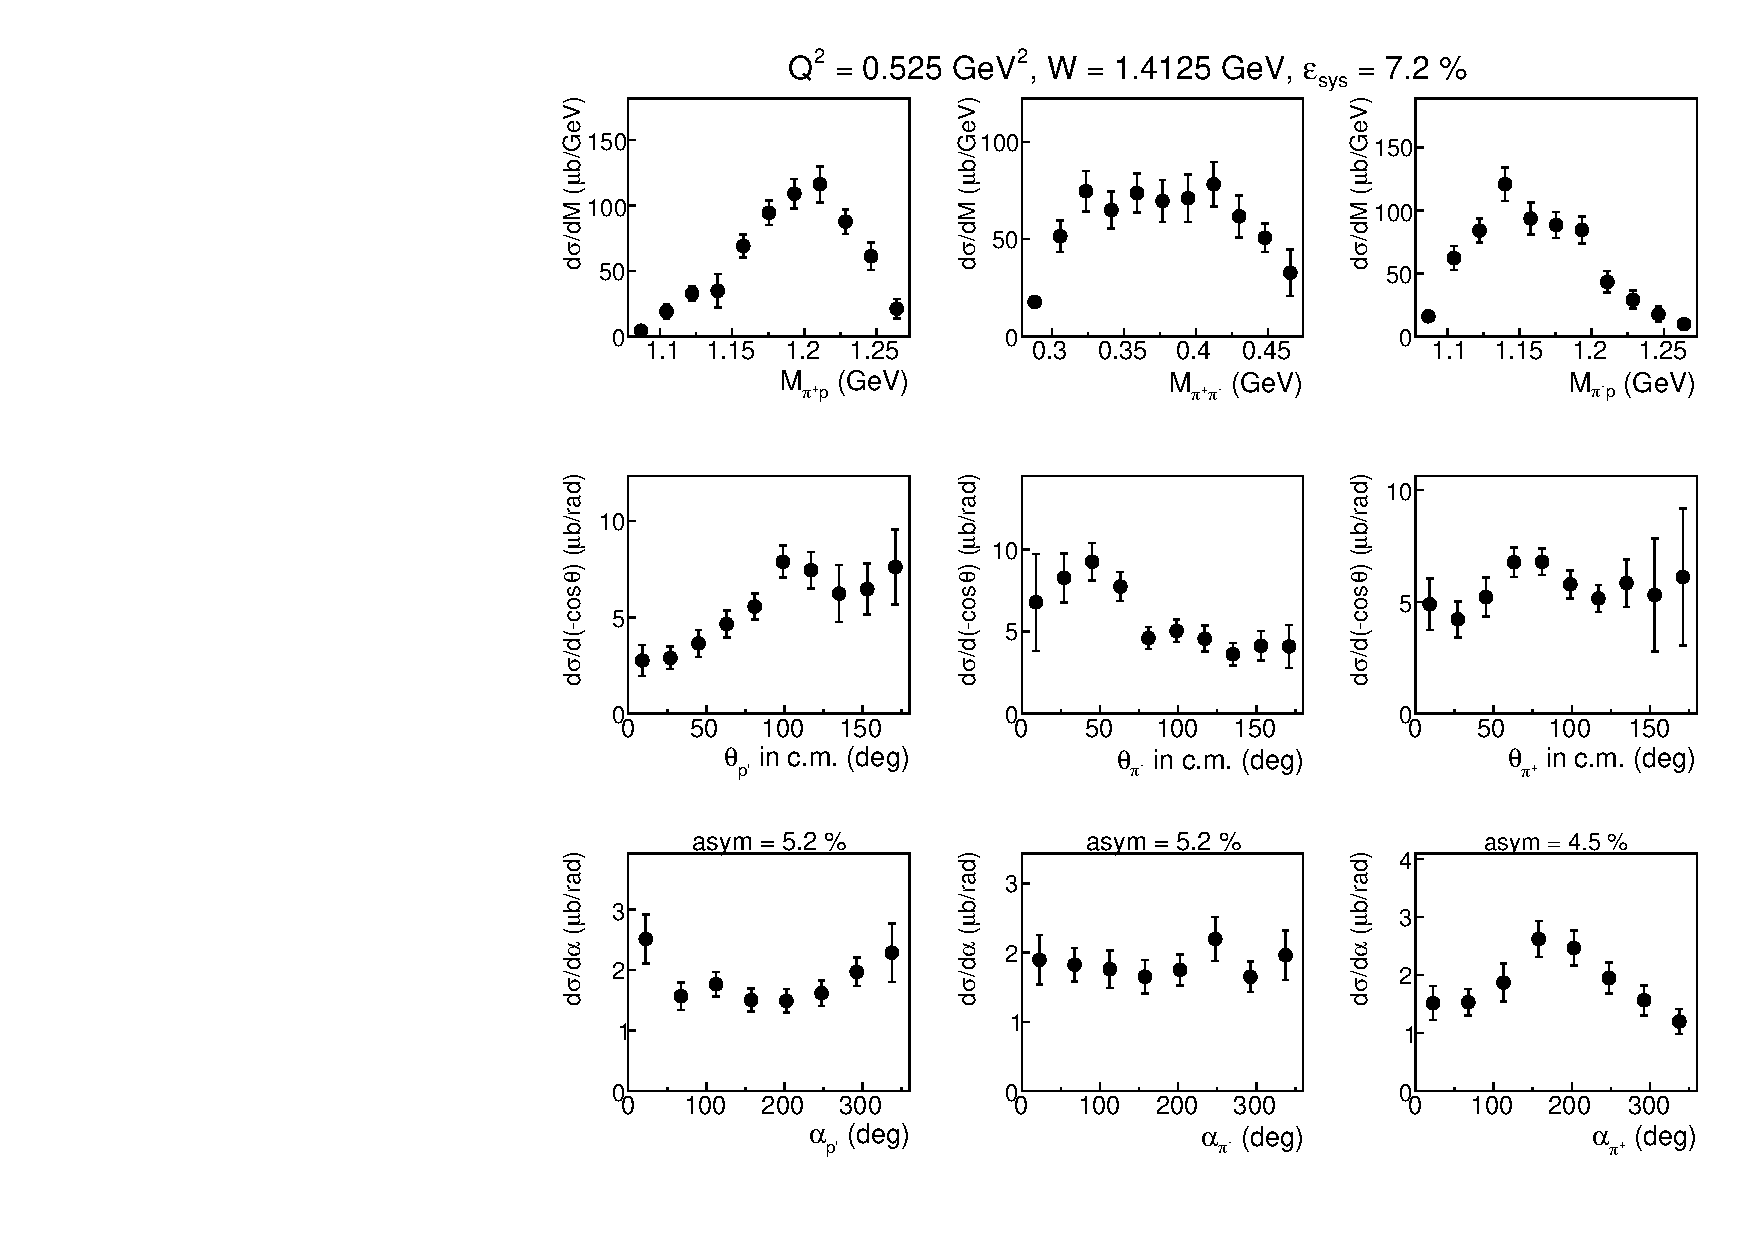
\includegraphics[width=0.45\textwidth]{pictures/appendix/1diff_distr/Q2_525/w_14125.pdf}}
\frame{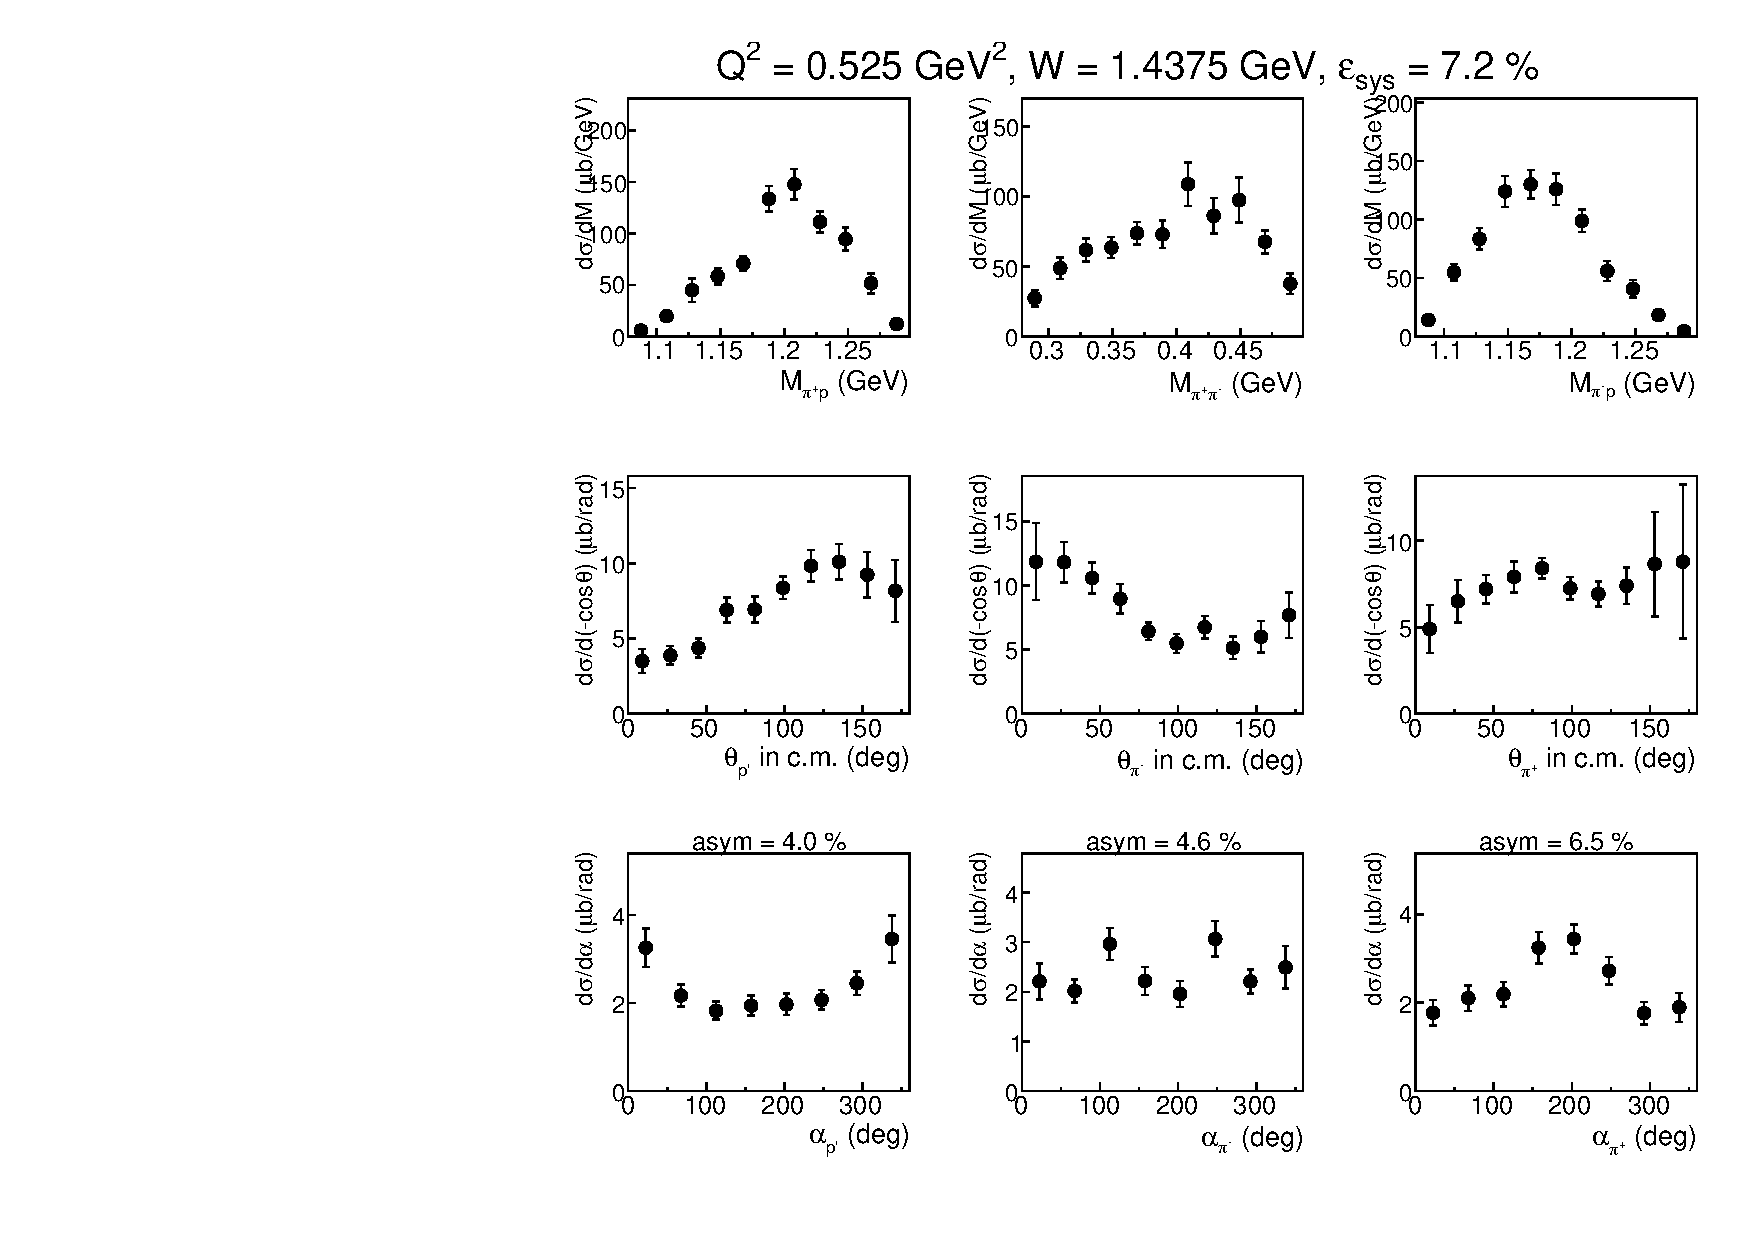
\includegraphics[width=0.45\textwidth]{pictures/appendix/1diff_distr/Q2_525/w_14375.pdf}}
\caption{\small } \label{fig:appx_9}
\end{center}
\end{figure}

\clearpage
\begin{figure}[htp]
\begin{center}
\frame{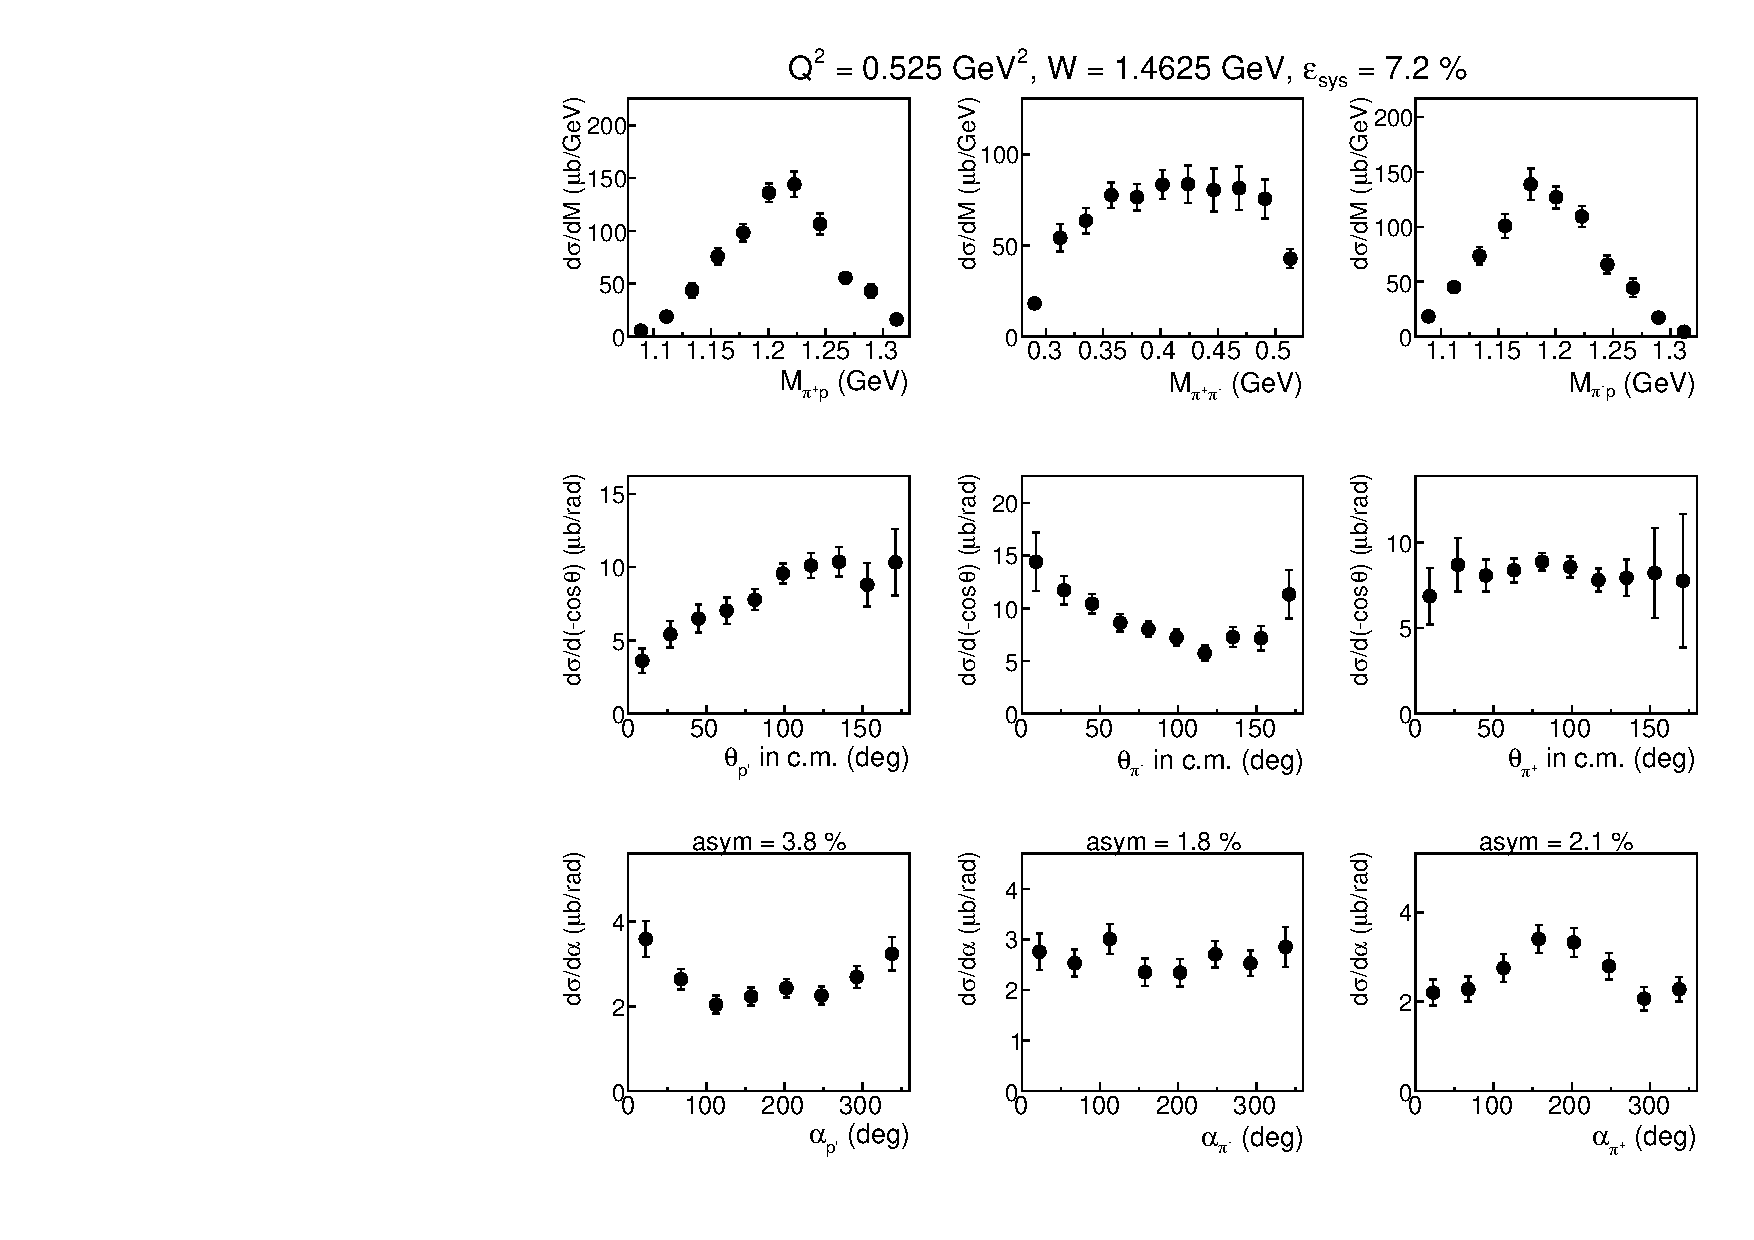
\includegraphics[width=0.45\textwidth]{pictures/appendix/1diff_distr/Q2_525/w_14625.pdf}}
\frame{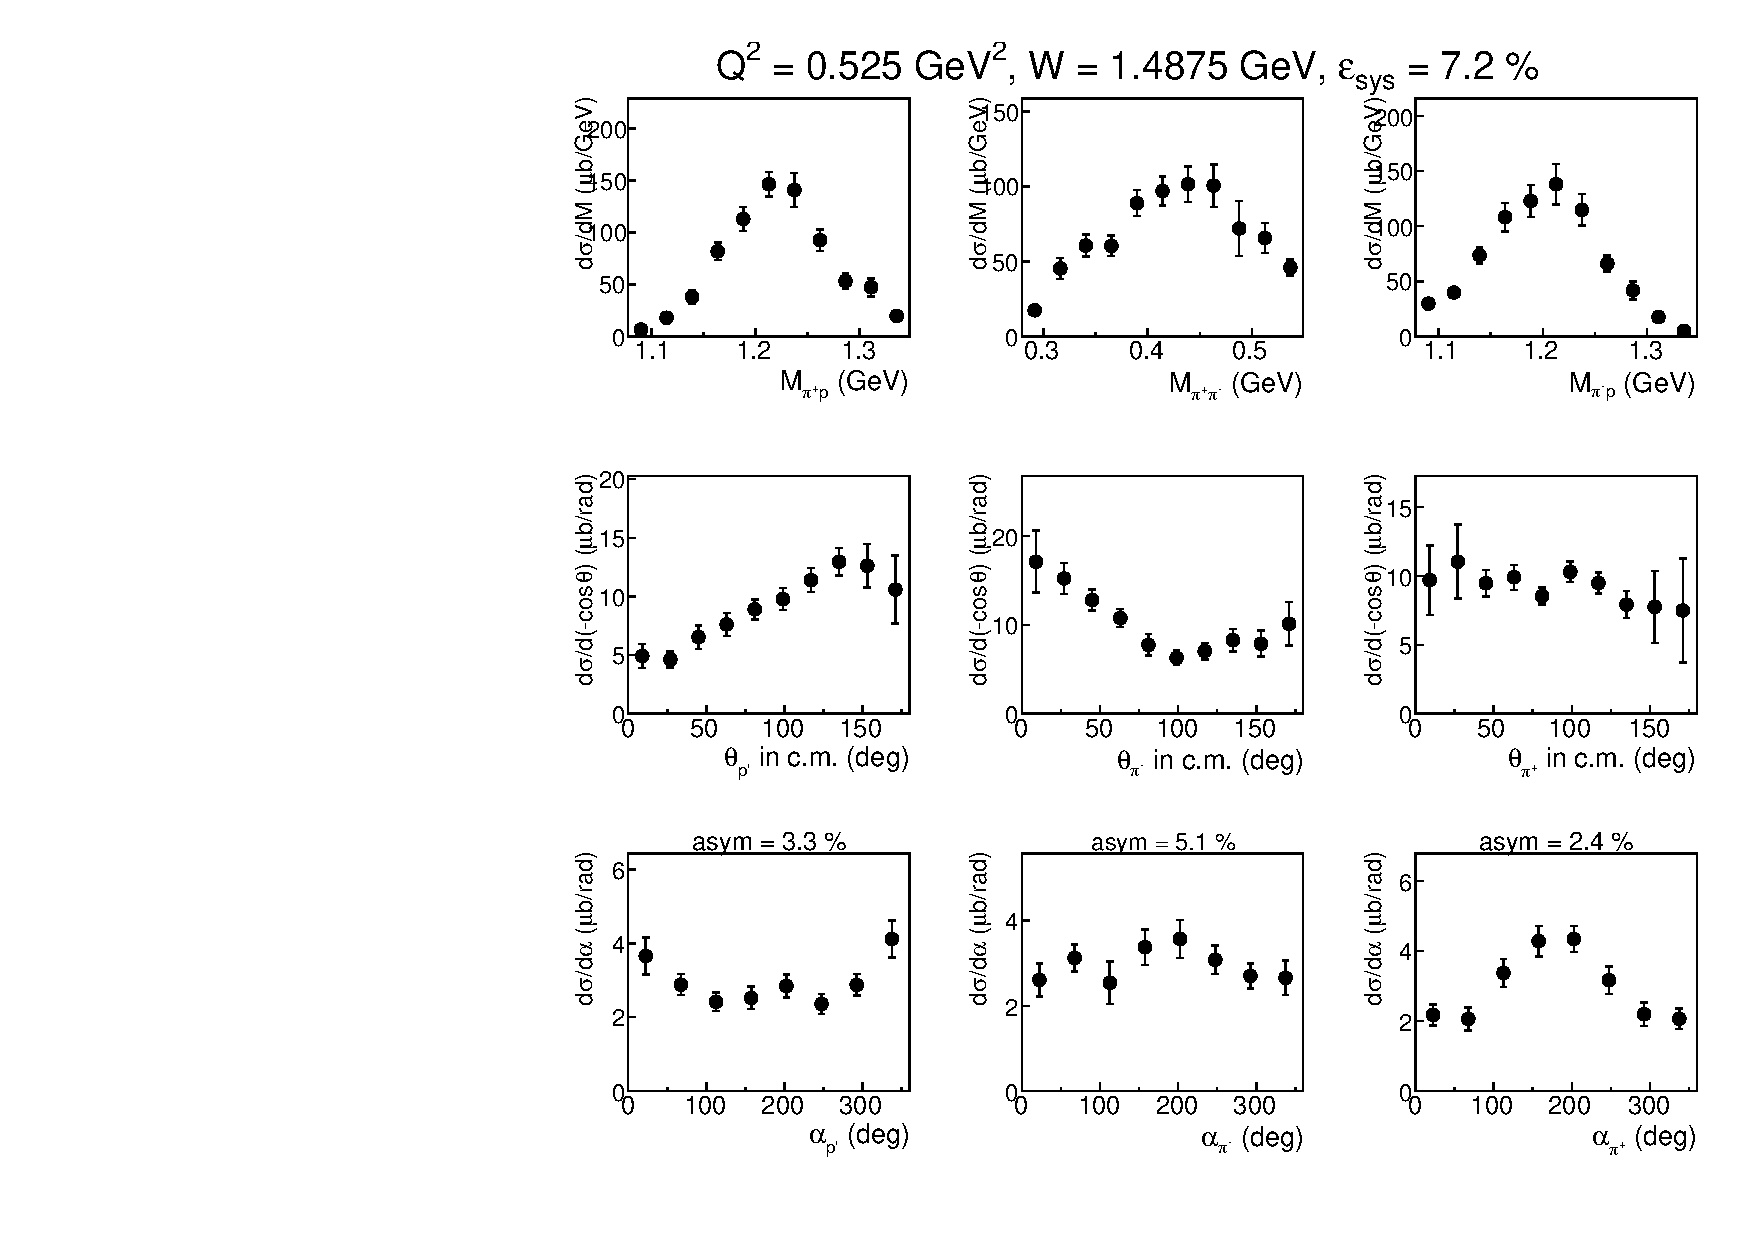
\includegraphics[width=0.45\textwidth]{pictures/appendix/1diff_distr/Q2_525/w_14875.pdf}}
\frame{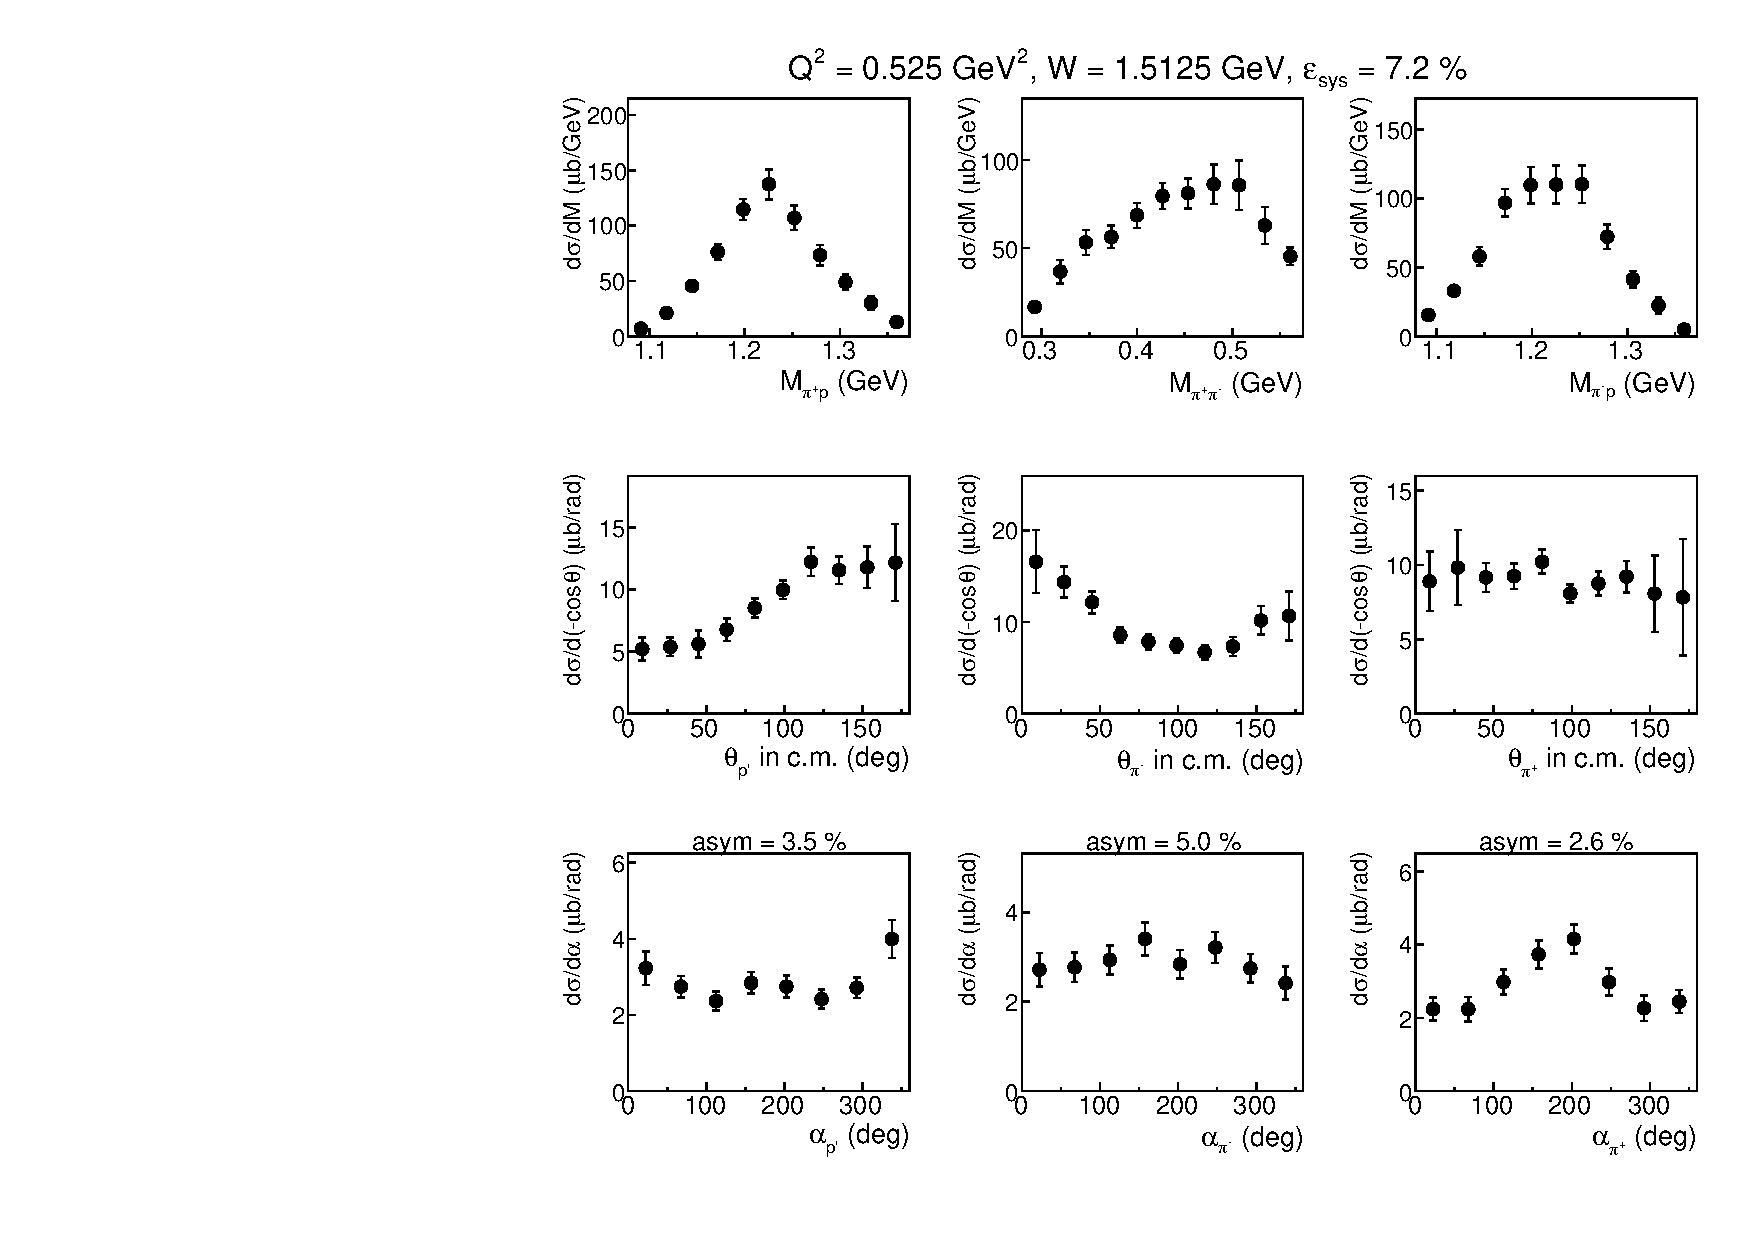
\includegraphics[width=0.45\textwidth]{pictures/appendix/1diff_distr/Q2_525/w_15125.pdf}}
\frame{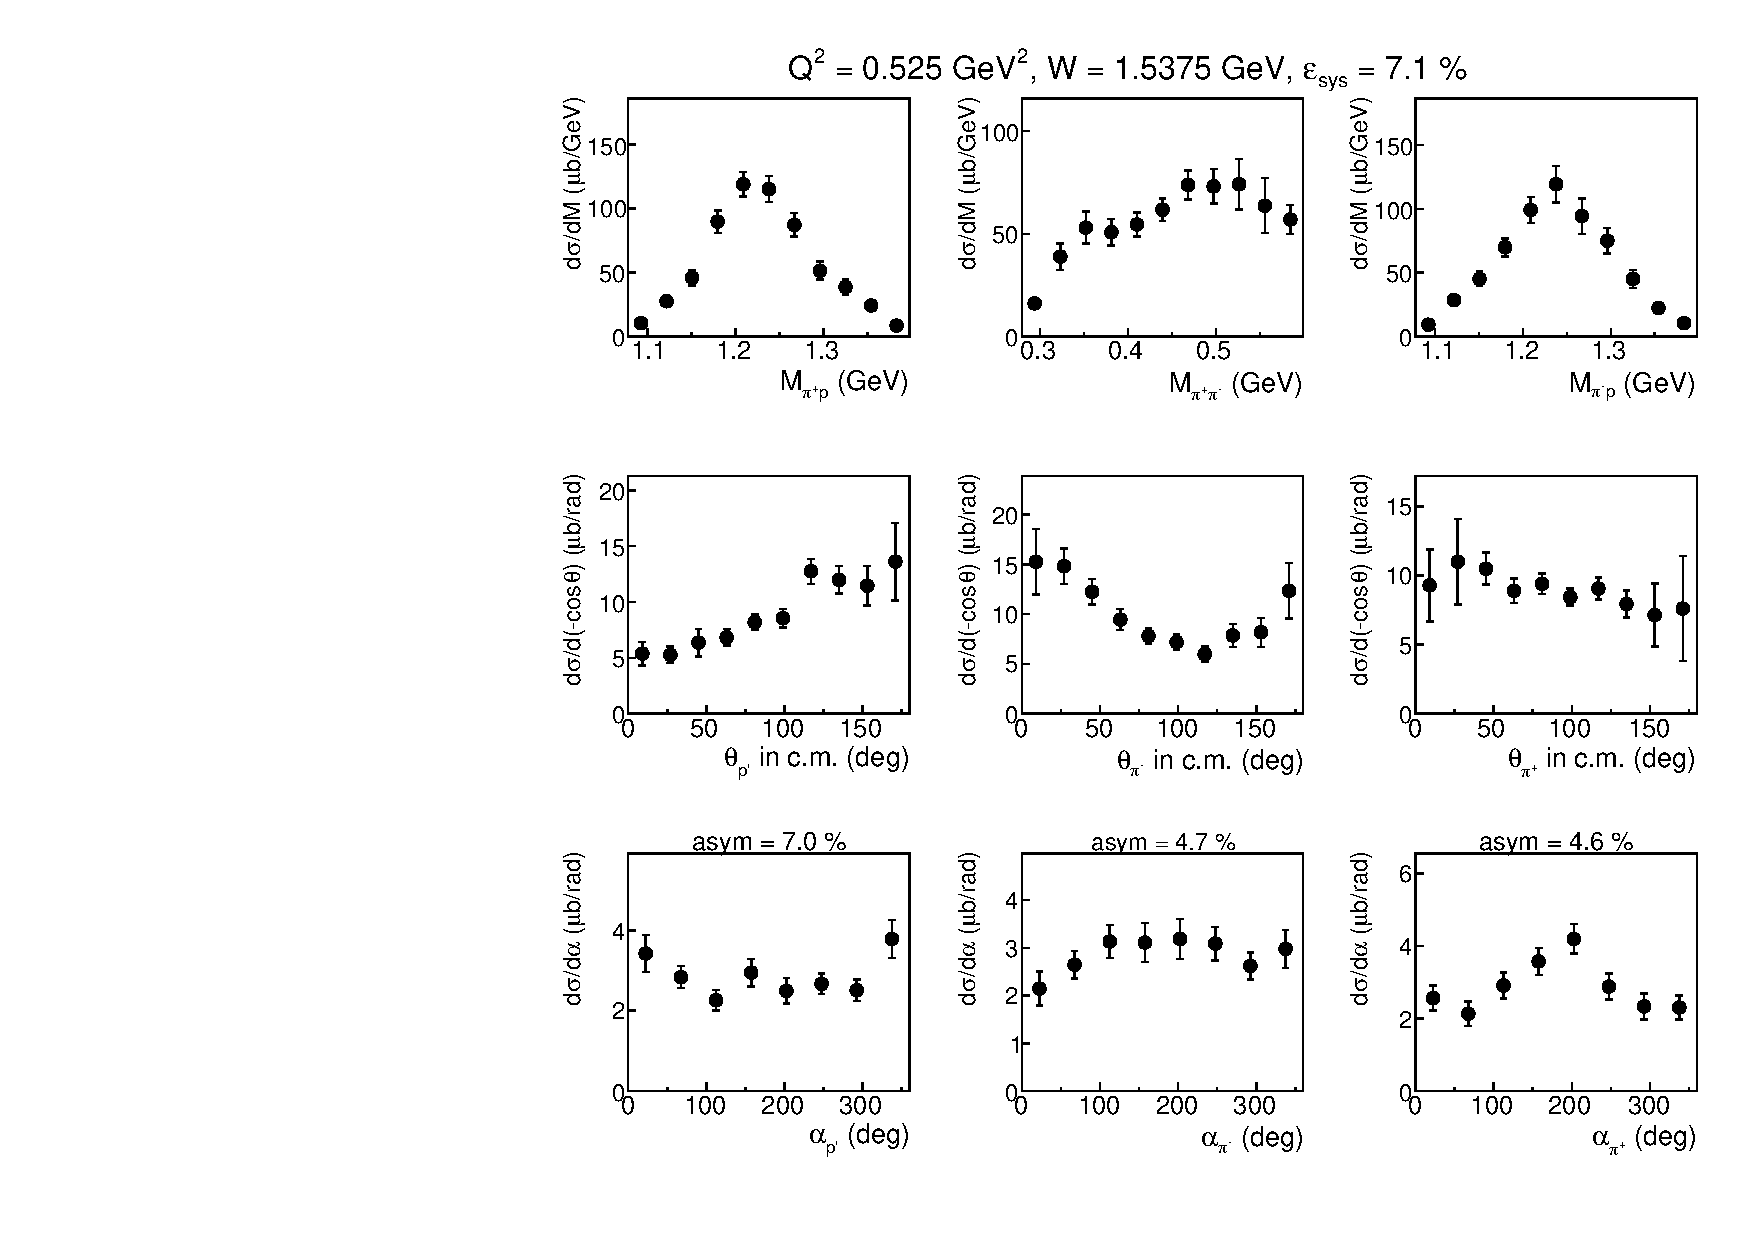
\includegraphics[width=0.45\textwidth]{pictures/appendix/1diff_distr/Q2_525/w_15375.pdf}}
\caption{\small } \label{fig:appx_10}
\end{center}
\end{figure}

\clearpage
\begin{figure}[htp]
\begin{center}
\frame{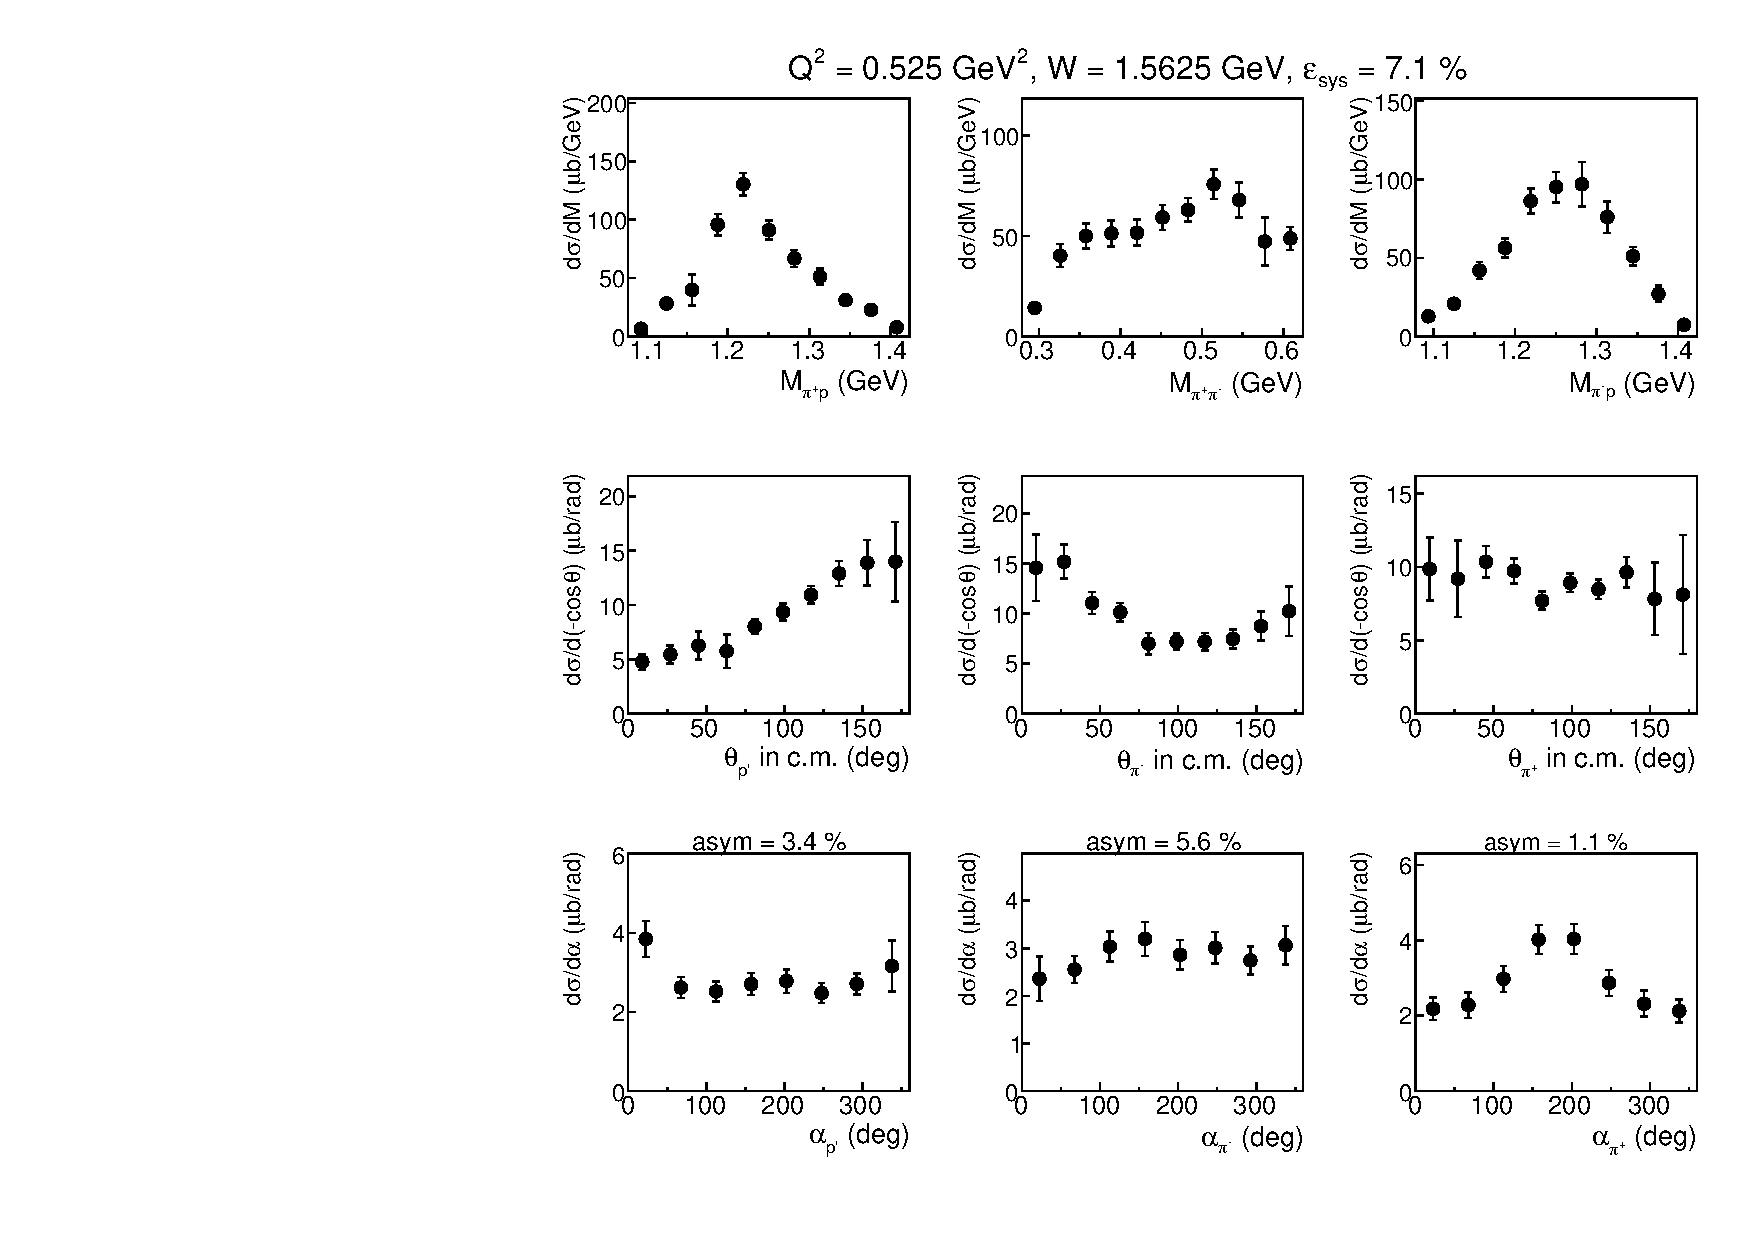
\includegraphics[width=0.45\textwidth]{pictures/appendix/1diff_distr/Q2_525/w_15625.pdf}}
\frame{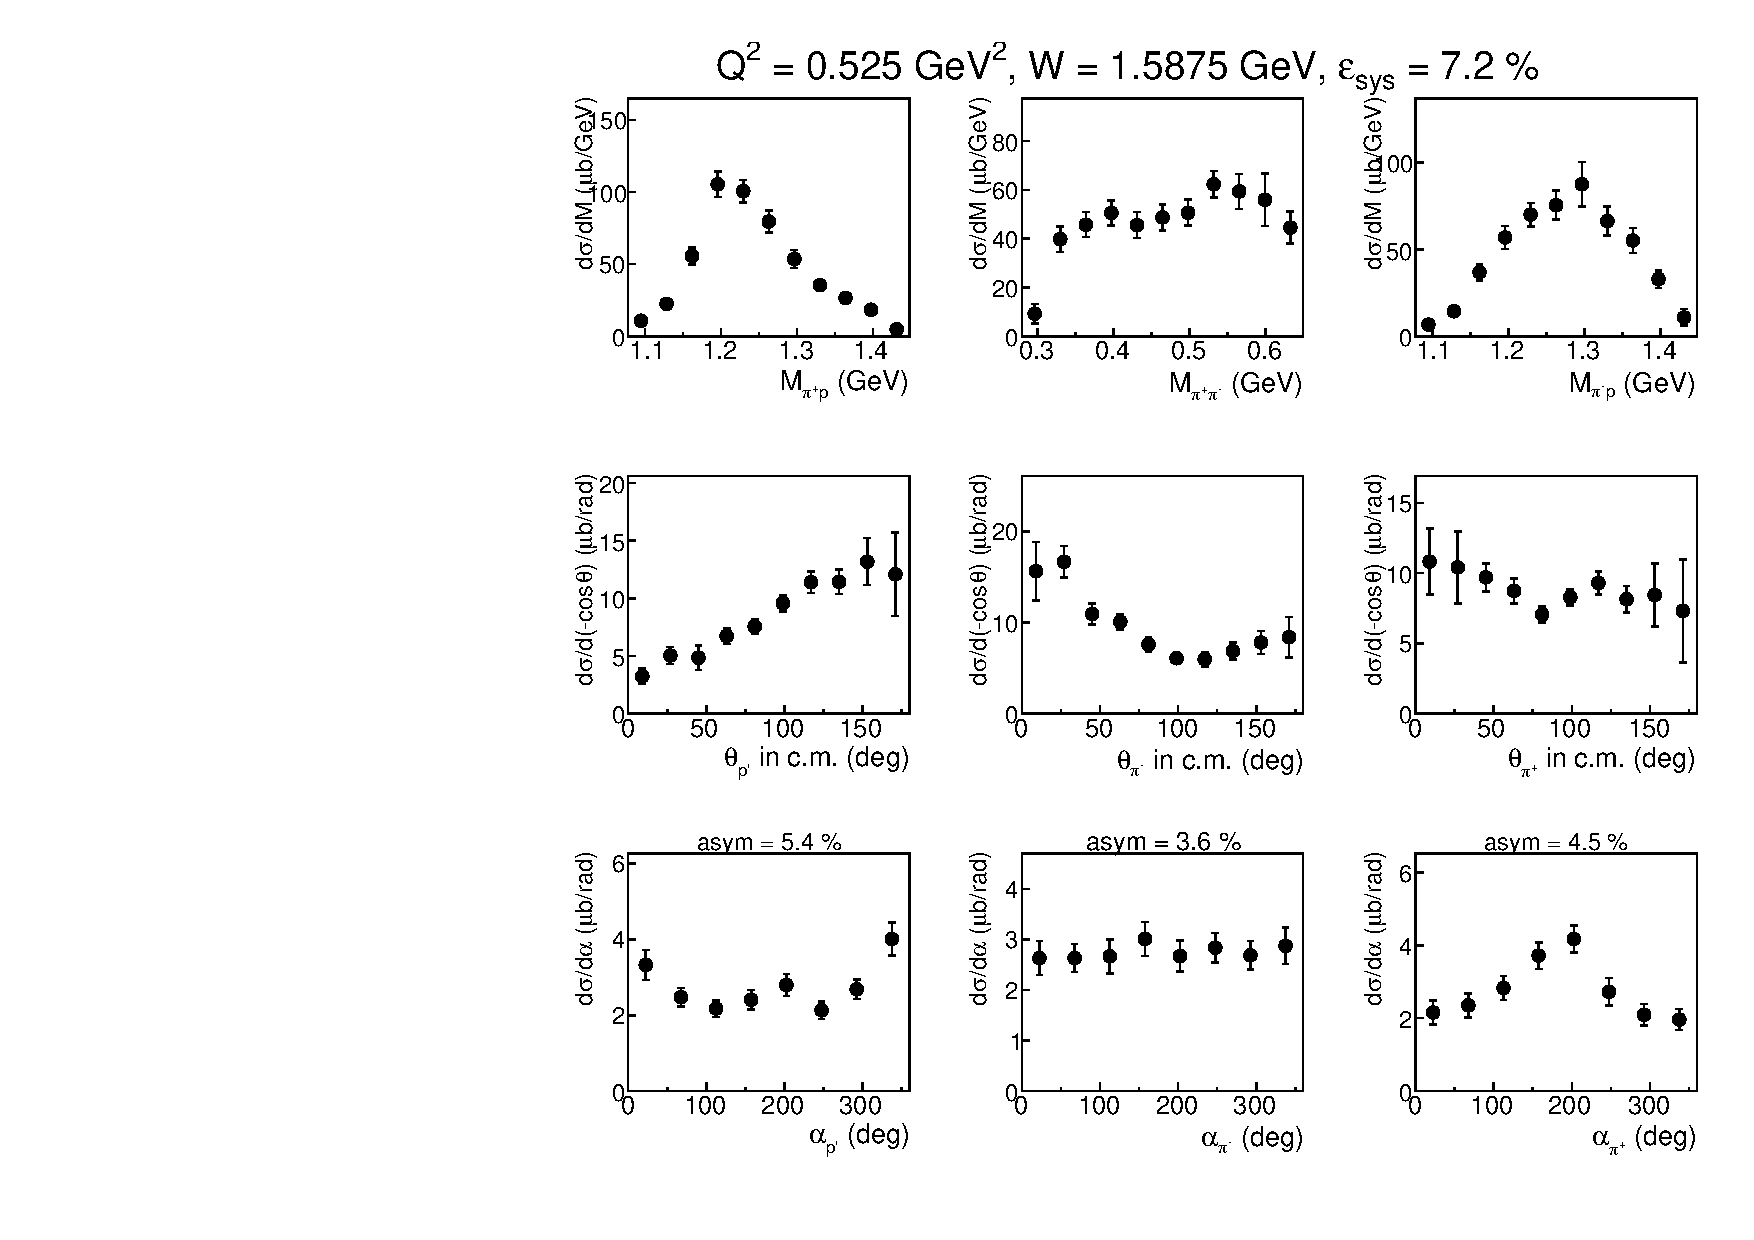
\includegraphics[width=0.45\textwidth]{pictures/appendix/1diff_distr/Q2_525/w_15875.pdf}}
\frame{\includegraphics[width=0.45\textwidth]{pictures/appendix/1diff_distr/Q2_525/w_16125.pdf}}
\frame{\includegraphics[width=0.45\textwidth]{pictures/appendix/1diff_distr/Q2_525/w_16375.pdf}}
\caption{\small } \label{fig:appx_11}
\end{center}
\end{figure}

\clearpage
\begin{figure}[htp]
\begin{center}
\frame{\includegraphics[width=0.45\textwidth]{pictures/appendix/1diff_distr/Q2_525/w_16625.pdf}}
\frame{\includegraphics[width=0.45\textwidth]{pictures/appendix/1diff_distr/Q2_525/w_16875.pdf}}
\frame{\includegraphics[width=0.45\textwidth]{pictures/appendix/1diff_distr/Q2_525/w_17125.pdf}}
\frame{\includegraphics[width=0.45\textwidth]{pictures/appendix/1diff_distr/Q2_525/w_17375.pdf}}
\caption{\small } \label{fig:appx_12}
\end{center}
\end{figure}

\clearpage
\begin{figure}[htp]
\begin{center}
\frame{\includegraphics[width=0.45\textwidth]{pictures/appendix/1diff_distr/Q2_525/w_17625.pdf}}
\frame{\includegraphics[width=0.45\textwidth]{pictures/appendix/1diff_distr/Q2_525/w_17875.pdf}}
\frame{\includegraphics[width=0.45\textwidth]{pictures/appendix/1diff_distr/Q2_575/w_13125.pdf}}
\frame{\includegraphics[width=0.45\textwidth]{pictures/appendix/1diff_distr/Q2_575/w_13375.pdf}}
\caption{\small } \label{fig:appx_13}
\end{center}
\end{figure}

\clearpage
\begin{figure}[htp]
\begin{center}
\frame{\includegraphics[width=0.45\textwidth]{pictures/appendix/1diff_distr/Q2_575/w_13625.pdf}}
\frame{\includegraphics[width=0.45\textwidth]{pictures/appendix/1diff_distr/Q2_575/w_13875.pdf}}
\frame{\includegraphics[width=0.45\textwidth]{pictures/appendix/1diff_distr/Q2_575/w_14125.pdf}}
\frame{\includegraphics[width=0.45\textwidth]{pictures/appendix/1diff_distr/Q2_575/w_14375.pdf}}
\caption{\small } \label{fig:appx_14}
\end{center}
\end{figure}

\clearpage
\begin{figure}[htp]
\begin{center}
\frame{\includegraphics[width=0.45\textwidth]{pictures/appendix/1diff_distr/Q2_575/w_14625.pdf}}
\frame{\includegraphics[width=0.45\textwidth]{pictures/appendix/1diff_distr/Q2_575/w_14875.pdf}}
\frame{\includegraphics[width=0.45\textwidth]{pictures/appendix/1diff_distr/Q2_575/w_15125.pdf}}
\frame{\includegraphics[width=0.45\textwidth]{pictures/appendix/1diff_distr/Q2_575/w_15375.pdf}}
\caption{\small } \label{fig:appx_15}
\end{center}
\end{figure}

\clearpage
\begin{figure}[htp]
\begin{center}
\frame{\includegraphics[width=0.45\textwidth]{pictures/appendix/1diff_distr/Q2_575/w_15625.pdf}}
\frame{\includegraphics[width=0.45\textwidth]{pictures/appendix/1diff_distr/Q2_575/w_15875.pdf}}
\frame{\includegraphics[width=0.45\textwidth]{pictures/appendix/1diff_distr/Q2_575/w_16125.pdf}}
\frame{\includegraphics[width=0.45\textwidth]{pictures/appendix/1diff_distr/Q2_575/w_16375.pdf}}
\caption{\small } \label{fig:appx_16}
\end{center}
\end{figure}

\clearpage
\begin{figure}[htp]
\begin{center}
\frame{\includegraphics[width=0.45\textwidth]{pictures/appendix/1diff_distr/Q2_575/w_16625.pdf}}
\frame{\includegraphics[width=0.45\textwidth]{pictures/appendix/1diff_distr/Q2_575/w_16875.pdf}}
\frame{\includegraphics[width=0.45\textwidth]{pictures/appendix/1diff_distr/Q2_575/w_17125.pdf}}
\frame{\includegraphics[width=0.45\textwidth]{pictures/appendix/1diff_distr/Q2_575/w_17375.pdf}}
\caption{\small } \label{fig:appx_17}
\end{center}
\end{figure}


\clearpage
\begin{figure}[htp]
\begin{center}
\frame{\includegraphics[width=0.45\textwidth]{pictures/appendix/1diff_distr/Q2_575/w_17625.pdf}}
\frame{\includegraphics[width=0.45\textwidth]{pictures/appendix/1diff_distr/Q2_575/w_17875.pdf}}
\frame{\includegraphics[width=0.45\textwidth]{pictures/appendix/1diff_distr/Q2_625/w_13125.pdf}}
\frame{\includegraphics[width=0.45\textwidth]{pictures/appendix/1diff_distr/Q2_625/w_13375.pdf}}
\caption{\small } \label{fig:appx_18}
\end{center}
\end{figure}

\clearpage
\begin{figure}[htp]
\begin{center}
\frame{\includegraphics[width=0.45\textwidth]{pictures/appendix/1diff_distr/Q2_625/w_13625.pdf}}
\frame{\includegraphics[width=0.45\textwidth]{pictures/appendix/1diff_distr/Q2_625/w_13875.pdf}}
\frame{\includegraphics[width=0.45\textwidth]{pictures/appendix/1diff_distr/Q2_625/w_14125.pdf}}
\frame{\includegraphics[width=0.45\textwidth]{pictures/appendix/1diff_distr/Q2_625/w_14375.pdf}}
\caption{\small } \label{fig:appx_19}
\end{center}
\end{figure}

\clearpage
\begin{figure}[htp]
\begin{center}
\frame{\includegraphics[width=0.45\textwidth]{pictures/appendix/1diff_distr/Q2_625/w_14625.pdf}}
\frame{\includegraphics[width=0.45\textwidth]{pictures/appendix/1diff_distr/Q2_625/w_14875.pdf}}
\frame{\includegraphics[width=0.45\textwidth]{pictures/appendix/1diff_distr/Q2_625/w_15125.pdf}}
\frame{\includegraphics[width=0.45\textwidth]{pictures/appendix/1diff_distr/Q2_625/w_15375.pdf}}
\caption{\small } \label{fig:appx_20}
\end{center}
\end{figure}

\clearpage
\begin{figure}[htp]
\begin{center}
\frame{\includegraphics[width=0.45\textwidth]{pictures/appendix/1diff_distr/Q2_625/w_15625.pdf}}
\frame{\includegraphics[width=0.45\textwidth]{pictures/appendix/1diff_distr/Q2_625/w_15875.pdf}}
\frame{\includegraphics[width=0.45\textwidth]{pictures/appendix/1diff_distr/Q2_625/w_16125.pdf}}
\frame{\includegraphics[width=0.45\textwidth]{pictures/appendix/1diff_distr/Q2_625/w_16375.pdf}}
\caption{\small } \label{fig:appx_21}
\end{center}
\end{figure}

\clearpage
\begin{figure}[htp]
\begin{center}
\frame{\includegraphics[width=0.45\textwidth]{pictures/appendix/1diff_distr/Q2_625/w_16625.pdf}}
\frame{\includegraphics[width=0.45\textwidth]{pictures/appendix/1diff_distr/Q2_625/w_16875.pdf}}
\frame{\includegraphics[width=0.45\textwidth]{pictures/appendix/1diff_distr/Q2_625/w_17125.pdf}}
\frame{\includegraphics[width=0.45\textwidth]{pictures/appendix/1diff_distr/Q2_625/w_17375.pdf}}
\caption{\small } \label{fig:appx_22}
\end{center}
\end{figure}

\clearpage
\begin{figure}[htp]
\begin{center}
\frame{\includegraphics[width=0.45\textwidth]{pictures/appendix/1diff_distr/Q2_625/w_17625.pdf}}
\frame{\includegraphics[width=0.45\textwidth]{pictures/appendix/1diff_distr/Q2_675/w_13125.pdf}}
\frame{\includegraphics[width=0.45\textwidth]{pictures/appendix/1diff_distr/Q2_675/w_13375.pdf}}
\frame{\includegraphics[width=0.45\textwidth]{pictures/appendix/1diff_distr/Q2_675/w_13625.pdf}}
\caption{\small } \label{fig:appx_23}
\end{center}
\end{figure}

\clearpage
\begin{figure}[htp]
\begin{center}
\frame{\includegraphics[width=0.45\textwidth]{pictures/appendix/1diff_distr/Q2_675/w_13875.pdf}}
\frame{\includegraphics[width=0.45\textwidth]{pictures/appendix/1diff_distr/Q2_675/w_14125.pdf}}
\frame{\includegraphics[width=0.45\textwidth]{pictures/appendix/1diff_distr/Q2_675/w_14375.pdf}}
\frame{\includegraphics[width=0.45\textwidth]{pictures/appendix/1diff_distr/Q2_675/w_14625.pdf}}
\caption{\small } \label{fig:appx_24}
\end{center}
\end{figure}

\clearpage
\begin{figure}[htp]
\begin{center}
\frame{\includegraphics[width=0.45\textwidth]{pictures/appendix/1diff_distr/Q2_675/w_14875.pdf}}
\frame{\includegraphics[width=0.45\textwidth]{pictures/appendix/1diff_distr/Q2_675/w_15125.pdf}}
\frame{\includegraphics[width=0.45\textwidth]{pictures/appendix/1diff_distr/Q2_675/w_15375.pdf}}
\frame{\includegraphics[width=0.45\textwidth]{pictures/appendix/1diff_distr/Q2_675/w_15625.pdf}}
\caption{\small } \label{fig:appx_25}
\end{center}
\end{figure}

\clearpage
\begin{figure}[htp]
\begin{center}
\frame{\includegraphics[width=0.45\textwidth]{pictures/appendix/1diff_distr/Q2_675/w_15875.pdf}}
\frame{\includegraphics[width=0.45\textwidth]{pictures/appendix/1diff_distr/Q2_675/w_16125.pdf}}
\frame{\includegraphics[width=0.45\textwidth]{pictures/appendix/1diff_distr/Q2_675/w_16375.pdf}}
\frame{\includegraphics[width=0.45\textwidth]{pictures/appendix/1diff_distr/Q2_675/w_16625.pdf}}
\caption{\small } \label{fig:appx_26}
\end{center}
\end{figure}

\clearpage
\begin{figure}[htp]
\begin{center}
\frame{\includegraphics[width=0.45\textwidth]{pictures/appendix/1diff_distr/Q2_675/w_16875.pdf}}
\frame{\includegraphics[width=0.45\textwidth]{pictures/appendix/1diff_distr/Q2_675/w_17125.pdf}}
\frame{\includegraphics[width=0.45\textwidth]{pictures/appendix/1diff_distr/Q2_675/w_17375.pdf}}
\frame{\includegraphics[width=0.45\textwidth]{pictures/appendix/1diff_distr/Q2_675/w_17625.pdf}}
\caption{\small } \label{fig:appx_27}
\end{center}
\end{figure}

\clearpage
\begin{figure}[htp]
\begin{center}
\frame{\includegraphics[width=0.45\textwidth]{pictures/appendix/1diff_distr/Q2_725/w_13125.pdf}}
\frame{\includegraphics[width=0.45\textwidth]{pictures/appendix/1diff_distr/Q2_725/w_13375.pdf}}
\frame{\includegraphics[width=0.45\textwidth]{pictures/appendix/1diff_distr/Q2_725/w_13625.pdf}}
\frame{\includegraphics[width=0.45\textwidth]{pictures/appendix/1diff_distr/Q2_725/w_13875.pdf}}
\caption{\small } \label{fig:appx_28}
\end{center}
\end{figure}

\clearpage
\begin{figure}[htp]
\begin{center}
\frame{\includegraphics[width=0.45\textwidth]{pictures/appendix/1diff_distr/Q2_725/w_14125.pdf}}
\frame{\includegraphics[width=0.45\textwidth]{pictures/appendix/1diff_distr/Q2_725/w_14375.pdf}}
\frame{\includegraphics[width=0.45\textwidth]{pictures/appendix/1diff_distr/Q2_725/w_14625.pdf}}
\frame{\includegraphics[width=0.45\textwidth]{pictures/appendix/1diff_distr/Q2_725/w_14875.pdf}}
\caption{\small } \label{fig:appx_29}
\end{center}
\end{figure}

\clearpage
\begin{figure}[htp]
\begin{center}
\frame{\includegraphics[width=0.45\textwidth]{pictures/appendix/1diff_distr/Q2_725/w_15125.pdf}}
\frame{\includegraphics[width=0.45\textwidth]{pictures/appendix/1diff_distr/Q2_725/w_15375.pdf}}
\frame{\includegraphics[width=0.45\textwidth]{pictures/appendix/1diff_distr/Q2_725/w_15625.pdf}}
\frame{\includegraphics[width=0.45\textwidth]{pictures/appendix/1diff_distr/Q2_725/w_15875.pdf}}
\caption{\small } \label{fig:appx_30}
\end{center}
\end{figure}

\clearpage
\begin{figure}[htp]
\begin{center}
\frame{\includegraphics[width=0.45\textwidth]{pictures/appendix/1diff_distr/Q2_725/w_16125.pdf}}
\frame{\includegraphics[width=0.45\textwidth]{pictures/appendix/1diff_distr/Q2_725/w_16375.pdf}}
\frame{\includegraphics[width=0.45\textwidth]{pictures/appendix/1diff_distr/Q2_725/w_16625.pdf}}
\frame{\includegraphics[width=0.45\textwidth]{pictures/appendix/1diff_distr/Q2_725/w_16875.pdf}}
\caption{\small } \label{fig:appx_31}
\end{center}
\end{figure}

\clearpage
\begin{figure}[htp]
\begin{center}
\frame{\includegraphics[width=0.45\textwidth]{pictures/appendix/1diff_distr/Q2_725/w_17125.pdf}}
\frame{\includegraphics[width=0.45\textwidth]{pictures/appendix/1diff_distr/Q2_725/w_17375.pdf}}
\frame{\includegraphics[width=0.45\textwidth]{pictures/appendix/1diff_distr/Q2_775/w_13125.pdf}}
\frame{\includegraphics[width=0.45\textwidth]{pictures/appendix/1diff_distr/Q2_775/w_13375.pdf}}
\caption{\small } \label{fig:appx_32}
\end{center}
\end{figure}

\clearpage
\begin{figure}[htp]
\begin{center}
\frame{\includegraphics[width=0.45\textwidth]{pictures/appendix/1diff_distr/Q2_775/w_13625.pdf}}
\frame{\includegraphics[width=0.45\textwidth]{pictures/appendix/1diff_distr/Q2_775/w_13875.pdf}}
\frame{\includegraphics[width=0.45\textwidth]{pictures/appendix/1diff_distr/Q2_775/w_14125.pdf}}
\frame{\includegraphics[width=0.45\textwidth]{pictures/appendix/1diff_distr/Q2_775/w_14375.pdf}}
\caption{\small } \label{fig:appx_33}
\end{center}
\end{figure}

\clearpage
\begin{figure}[htp]
\begin{center}
\frame{\includegraphics[width=0.45\textwidth]{pictures/appendix/1diff_distr/Q2_775/w_14625.pdf}}
\frame{\includegraphics[width=0.45\textwidth]{pictures/appendix/1diff_distr/Q2_775/w_14875.pdf}}
\frame{\includegraphics[width=0.45\textwidth]{pictures/appendix/1diff_distr/Q2_775/w_15125.pdf}}
\frame{\includegraphics[width=0.45\textwidth]{pictures/appendix/1diff_distr/Q2_775/w_15375.pdf}}
\caption{\small } \label{fig:appx_34}
\end{center}
\end{figure}

\clearpage
\begin{figure}[htp]
\begin{center}
\frame{\includegraphics[width=0.45\textwidth]{pictures/appendix/1diff_distr/Q2_775/w_15625.pdf}}
\frame{\includegraphics[width=0.45\textwidth]{pictures/appendix/1diff_distr/Q2_775/w_15875.pdf}}
\frame{\includegraphics[width=0.45\textwidth]{pictures/appendix/1diff_distr/Q2_775/w_16125.pdf}}
\frame{\includegraphics[width=0.45\textwidth]{pictures/appendix/1diff_distr/Q2_775/w_16375.pdf}}
\caption{\small } \label{fig:appx_35}
\end{center}
\end{figure}

\clearpage
\begin{figure}[htp]
\begin{center}
\frame{\includegraphics[width=0.45\textwidth]{pictures/appendix/1diff_distr/Q2_775/w_16625.pdf}}
\frame{\includegraphics[width=0.45\textwidth]{pictures/appendix/1diff_distr/Q2_775/w_16875.pdf}}
\frame{\includegraphics[width=0.45\textwidth]{pictures/appendix/1diff_distr/Q2_775/w_17125.pdf}}
\frame{\includegraphics[width=0.45\textwidth]{pictures/appendix/1diff_distr/Q2_825/w_13125.pdf}}
\caption{\small } \label{fig:appx_36}
\end{center}
\end{figure}

\clearpage
\begin{figure}[htp]
\begin{center}
\frame{\includegraphics[width=0.45\textwidth]{pictures/appendix/1diff_distr/Q2_825/w_13375.pdf}}
\frame{\includegraphics[width=0.45\textwidth]{pictures/appendix/1diff_distr/Q2_825/w_13625.pdf}}
\frame{\includegraphics[width=0.45\textwidth]{pictures/appendix/1diff_distr/Q2_825/w_13875.pdf}}
\frame{\includegraphics[width=0.45\textwidth]{pictures/appendix/1diff_distr/Q2_825/w_14125.pdf}}
\caption{\small } \label{fig:appx_37}
\end{center}
\end{figure}

\clearpage
\begin{figure}[htp]
\begin{center}
\frame{\includegraphics[width=0.45\textwidth]{pictures/appendix/1diff_distr/Q2_825/w_14375.pdf}}
\frame{\includegraphics[width=0.45\textwidth]{pictures/appendix/1diff_distr/Q2_825/w_14625.pdf}}
\frame{\includegraphics[width=0.45\textwidth]{pictures/appendix/1diff_distr/Q2_825/w_14875.pdf}}
\frame{\includegraphics[width=0.45\textwidth]{pictures/appendix/1diff_distr/Q2_825/w_15125.pdf}}
\caption{\small } \label{fig:appx_38}
\end{center}
\end{figure}

\clearpage
\begin{figure}[htp]
\begin{center}
\frame{\includegraphics[width=0.45\textwidth]{pictures/appendix/1diff_distr/Q2_825/w_15375.pdf}}
\frame{\includegraphics[width=0.45\textwidth]{pictures/appendix/1diff_distr/Q2_825/w_15625.pdf}}
\frame{\includegraphics[width=0.45\textwidth]{pictures/appendix/1diff_distr/Q2_825/w_15875.pdf}}
\frame{\includegraphics[width=0.45\textwidth]{pictures/appendix/1diff_distr/Q2_825/w_16125.pdf}}
\caption{\small } \label{fig:appx_39}
\end{center}
\end{figure}

\clearpage
\begin{figure}[htp]
\begin{center}
\frame{\includegraphics[width=0.45\textwidth]{pictures/appendix/1diff_distr/Q2_825/w_16375.pdf}}
\frame{\includegraphics[width=0.45\textwidth]{pictures/appendix/1diff_distr/Q2_825/w_16625.pdf}}
\frame{\includegraphics[width=0.45\textwidth]{pictures/appendix/1diff_distr/Q2_825/w_16875.pdf}}
\frame{\includegraphics[width=0.45\textwidth]{pictures/appendix/1diff_distr/Q2_875/w_13125.pdf}}
\caption{\small } \label{fig:appx_40}
\end{center}
\end{figure}

\clearpage
\begin{figure}[htp]
\begin{center}
\frame{\includegraphics[width=0.45\textwidth]{pictures/appendix/1diff_distr/Q2_875/w_13375.pdf}}
\frame{\includegraphics[width=0.45\textwidth]{pictures/appendix/1diff_distr/Q2_875/w_13625.pdf}}
\frame{\includegraphics[width=0.45\textwidth]{pictures/appendix/1diff_distr/Q2_875/w_13875.pdf}}
\frame{\includegraphics[width=0.45\textwidth]{pictures/appendix/1diff_distr/Q2_875/w_14125.pdf}}
\caption{\small } \label{fig:appx_41}
\end{center}
\end{figure}

\clearpage
\begin{figure}[htp]
\begin{center}
\frame{\includegraphics[width=0.45\textwidth]{pictures/appendix/1diff_distr/Q2_875/w_14375.pdf}}
\frame{\includegraphics[width=0.45\textwidth]{pictures/appendix/1diff_distr/Q2_875/w_14625.pdf}}
\frame{\includegraphics[width=0.45\textwidth]{pictures/appendix/1diff_distr/Q2_875/w_14875.pdf}}
\frame{\includegraphics[width=0.45\textwidth]{pictures/appendix/1diff_distr/Q2_875/w_15125.pdf}}
\caption{\small } \label{fig:appx_42}
\end{center}
\end{figure}

\clearpage
\begin{figure}[htp]
\begin{center}
\frame{\includegraphics[width=0.45\textwidth]{pictures/appendix/1diff_distr/Q2_875/w_15375.pdf}}
\frame{\includegraphics[width=0.45\textwidth]{pictures/appendix/1diff_distr/Q2_875/w_15625.pdf}}
\frame{\includegraphics[width=0.45\textwidth]{pictures/appendix/1diff_distr/Q2_875/w_15875.pdf}}
\frame{\includegraphics[width=0.45\textwidth]{pictures/appendix/1diff_distr/Q2_875/w_16125.pdf}}
\caption{\small } \label{fig:appx_43}
\end{center}
\end{figure}

\clearpage
\begin{figure}[htp]
\begin{center}
\frame{\includegraphics[width=0.45\textwidth]{pictures/appendix/1diff_distr/Q2_875/w_16375.pdf}}
\frame{\includegraphics[width=0.45\textwidth]{pictures/appendix/1diff_distr/Q2_875/w_16625.pdf}}
\frame{\includegraphics[width=0.45\textwidth]{pictures/appendix/1diff_distr/Q2_925/w_13125.pdf}}
\frame{\includegraphics[width=0.45\textwidth]{pictures/appendix/1diff_distr/Q2_925/w_13375.pdf}}
\caption{\small } \label{fig:appx_44}
\end{center}
\end{figure}

\clearpage
\begin{figure}[htp]
\begin{center}
\frame{\includegraphics[width=0.45\textwidth]{pictures/appendix/1diff_distr/Q2_925/w_13625.pdf}}
\frame{\includegraphics[width=0.45\textwidth]{pictures/appendix/1diff_distr/Q2_925/w_13875.pdf}}
\frame{\includegraphics[width=0.45\textwidth]{pictures/appendix/1diff_distr/Q2_925/w_14125.pdf}}
\frame{\includegraphics[width=0.45\textwidth]{pictures/appendix/1diff_distr/Q2_925/w_14375.pdf}}
\caption{\small } \label{fig:appx_45}
\end{center}
\end{figure}

\clearpage
\begin{figure}[htp]
\begin{center}
\frame{\includegraphics[width=0.45\textwidth]{pictures/appendix/1diff_distr/Q2_925/w_14625.pdf}}
\frame{\includegraphics[width=0.45\textwidth]{pictures/appendix/1diff_distr/Q2_925/w_14875.pdf}}
\frame{\includegraphics[width=0.45\textwidth]{pictures/appendix/1diff_distr/Q2_925/w_15125.pdf}}
\frame{\includegraphics[width=0.45\textwidth]{pictures/appendix/1diff_distr/Q2_925/w_15375.pdf}}
\caption{\small } \label{fig:appx_46}
\end{center}
\end{figure}

\clearpage
\begin{figure}[htp]
\begin{center}
\frame{\includegraphics[width=0.45\textwidth]{pictures/appendix/1diff_distr/Q2_925/w_15625.pdf}}
\frame{\includegraphics[width=0.45\textwidth]{pictures/appendix/1diff_distr/Q2_925/w_15875.pdf}}
\frame{\includegraphics[width=0.45\textwidth]{pictures/appendix/1diff_distr/Q2_925/w_16125.pdf}}
\frame{\includegraphics[width=0.45\textwidth]{pictures/appendix/1diff_distr/Q2_975/w_13125.pdf}}
\caption{\small } \label{fig:appx_47}
\end{center}
\end{figure}

\clearpage
\begin{figure}[htp]
\begin{center}
\frame{\includegraphics[width=0.45\textwidth]{pictures/appendix/1diff_distr/Q2_975/w_13375.pdf}}
\frame{\includegraphics[width=0.45\textwidth]{pictures/appendix/1diff_distr/Q2_975/w_13625.pdf}}
\frame{\includegraphics[width=0.45\textwidth]{pictures/appendix/1diff_distr/Q2_975/w_13875.pdf}}
\frame{\includegraphics[width=0.45\textwidth]{pictures/appendix/1diff_distr/Q2_975/w_14125.pdf}}
\caption{\small } \label{fig:appx_48}
\end{center}
\end{figure}

\clearpage
\begin{figure}[htp]
\begin{center}
\frame{\includegraphics[width=0.45\textwidth]{pictures/appendix/1diff_distr/Q2_975/w_14375.pdf}}
\frame{\includegraphics[width=0.45\textwidth]{pictures/appendix/1diff_distr/Q2_975/w_14625.pdf}}
\frame{\includegraphics[width=0.45\textwidth]{pictures/appendix/1diff_distr/Q2_975/w_14875.pdf}}
\frame{\includegraphics[width=0.45\textwidth]{pictures/appendix/1diff_distr/Q2_975/w_15125.pdf}}
\caption{\small } \label{fig:appx_49}
\end{center}
\end{figure}

\clearpage
\begin{figure}[htp]
\begin{center}
\frame{\includegraphics[width=0.45\textwidth]{pictures/appendix/1diff_distr/Q2_975/w_15375.pdf}}
\frame{\includegraphics[width=0.45\textwidth]{pictures/appendix/1diff_distr/Q2_975/w_15625.pdf}}
\caption{\small } \label{fig:appx_50}
\end{center}
\end{figure}

%\end{comment}
